%& -job-name="[SD] Zadania v0.27"
\documentclass[a4paper,10pt]{article}
\usepackage[T1]{fontenc}
\usepackage[utf8]{inputenc}
\usepackage{amssymb}
\usepackage[polish]{babel}
\usepackage{amsthm}
\usepackage{amsmath}
\usepackage{times}
\usepackage{anysize}
\usepackage{enumerate}
\usepackage{color}
\usepackage{circuitikz}
\usepackage{multicol}
\tikzset{>=latex}
\usetikzlibrary{patterns}

\usepackage{siunitx}
\usepackage{mathrsfs}
\usepackage{cancel}


\marginsize{1cm}{1cm}{1cm}{1cm}
\definecolor{darkgray}{gray}{0.3}
\definecolor{darkblue}{RGB}{0,0,180}
\definecolor{red}{RGB}{255,0,0}
\definecolor{lightgray}{gray}{0.6}
\sloppy 

%dla zakreskowania ukośnymi liniami
\pgfdeclarepatternformonly[\LineSpace]{my north east lines}{\pgfqpoint{-1pt}{-1pt}}{\pgfqpoint{\LineSpace}{\LineSpace}}{\pgfqpoint{\LineSpace}{\LineSpace}}%
{
    \pgfsetlinewidth{0.4pt}
    \pgfpathmoveto{\pgfqpoint{0pt}{0pt}}
    \pgfpathlineto{\pgfqpoint{\LineSpace + 0.1pt}{\LineSpace + 0.1pt}}
    \pgfusepath{stroke}
}

\newdimen\LineSpace
\tikzset{
    line space/.code={\LineSpace=#1},
    line space=3pt
}
%end

\newcommand*\circled[1]{\tikz[baseline=(char.base)]{
            \node[shape=circle,draw,inner sep=1pt] (char) {\small{#1}};}}

\newcommand*\lineh{\noindent\makebox[\linewidth]{\rule{\paperwidth}{0.4pt}}}

\begin{document}
\noindent https://github.com/Jock69pl/SystemyDynamiczne.git  - oryginalni autorzy\\
\noindent https://github.com/Jock69pl/SystemyDynamiczne.git  - wersja rozwojowa\\
\\
Jeśli masz wolnego czasu trochę i chcesz pomóc doślij jakieś rozwiązanie.\\
Bardzo potrzebne są korekty, napewno jest tu sporo błędów.\\
Potrzebni są też komentatorzy, chodzi o całkowicie łopatologiczny komentarz typu "tu liczymy delte bo..."\\
\\
Z tego przedmiotu jest egzamin, więc warto to zrobić


\pagebreak
\section*{Tydzień 1}
Systemy liniowe 1-go rzedu\\
\begin{figure}[!h]
\begin{tikzpicture}
	\node at(0,0){$\dot{x}(t)=A\underbrace{x(t)}_{\in \mathbb{R}^n}+B\underbrace{u(t)}_{\in \mathbb{R}^r}$};
	\node at(-.5,1.3){{$n\times n$}};
	\node at(1.5,1.3){{$n\times r$}};
	\node at(.5,1.7){Stan};
	\node at(2.5,1.7){Sterowanie};

	\draw[->](-.5,1.2)--(-.4,.5);
	\draw[->](1.5,1.2)--(.9,.5);
	\draw[->](.5,1.6)--(.1,.5);
	\draw[->](2.5,1.6)--(1.5,.5);
\end{tikzpicture}
\end{figure}
\\
rozwiązanie:\\
$x(t)=e^{tA}x_0+\int^t_0e^{(t-r)A}Bu(r) \ dr$\\
\\
dla autonomicznych ($r=n=1, t\geqslant 0, u(t)\equiv 0$)\\
$x(t)=e^{tA}x_0$\\





\pagebreak
%###################                 1.1.1              #################################%
\subsection*{Zadanie 1.1.1} {\color{darkgray}
	Naszkicować rozwiązania równania różniczkowego:\\
	$\dot{x}(t)=\alpha_ix(t)$\\
	dla $x(0)=1, t\geqslant 0$ przy czym $i=1,2,3$ zaś\\
	$\alpha_1=1,  \ \ \ \alpha_2=2, \ \ \ \alpha_3=-1$\\
}\lineh
\\\\
{\color{lightgray}
$\frac{dx}{dt}=\alpha_ix$\\
$\frac{dx}{x}=\alpha_idt$\\
całkowanie:\\
$\ln|x|=\alpha_i t+{c}$\\
}
$x=ce^{\alpha_it}$\\
$x(0)=c=1$\\
$x=e^{\alpha_it}$\\
\\
$x=e^t \ \vee \ x=e^{2t} \ \vee \ x=e^{-t}$\\
($t\geqslant 0$, więc tylko prawa strona)\\

\begin{figure}[!h]
\begin{tikzpicture}
	\draw [color=blue, thick]%(-3.0,0.02)--(-2.75,0.03)--(-2.5,0.04)--(-2.25,0.05)--(-2.0,0.06)--(-1.75,0.08)--(-1.5,0.11)--(-1.25,0.14)--(-1.0,0.18)--(-0.75,0.23)--(-0.5,0.3)--(-0.25,0.38)--
(0.0,0.5)--(0.25,0.64)--(0.5,0.82)--(0.75,1.05)--(1.0,1.35)--(1.25,1.74)--(1.5,2.24)--(1.75,2.87);
	\draw [color=blue, thick]%(-3.0,0.0)--(-2.75,0.0)--(-2.5,0.0)--(-2.25,0.0)--(-2.0,0.0)--(-1.75,0.01)--(-1.5,0.02)--(-1.25,0.04)--(-1.0,0.06)--(-0.75,0.11)--(-0.5,0.18)--(-0.25,0.3)--
(0.0,0.5)--(0.25,0.82)--(0.5,1.35)--(0.75,2.24)--(1.0,3.69);
	\draw [color=blue, thick]%(-2.0,3.69)--(-1.75,2.87)--(-1.5,2.24)--(-1.25,1.74)--(-1.0,1.35)--(-0.75,1.05)--(-0.5,0.82)--(-0.25,0.64)--
(0.0,0.5)--(0.25,0.38)--(0.5,0.3)--(0.75,0.23)--(1.0,0.18)--(1.25,0.14)--(1.5,0.11)--(1.75,0.08)--(2.0,0.06)--(2.25,0.05)--(2.5,0.04)--(2.75,0.03)--(3.0,0.02);


	\node at(2,3){$\alpha_1$};
	\node at(1.2,3.8){$\alpha_2$};
	\node at(3,.2){$\alpha_3$};


	\draw[thick][->](-3,0)--(3,0) node [right=3pt]{$t$};
	\draw[thick][->](0,-3)--(0,3) node [right=3pt]{$x$};



	\draw (-0.1,.5) -- (0.1,.5) node [left=3pt]{{1}};
	\draw (1,-0.1) -- (1,0.1) node [below=4pt]{{1}};
\end{tikzpicture}
\end{figure}



\pagebreak
%###################                 1.2.1              #################################%
\subsection*{Zadanie 1.2.1} {\color{darkgray}
	Naszkicować rozwiazania równania rózniczkowego:\\
	$\dot{x}(t)=\alpha_ix(t)$\\
	dla $x(0)=-1, t\geqslant 0$ przy czym $i=1,2,3$ zaś\\
	$\alpha_1=-1,  \ \ \ \alpha_2=-2, \ \ \ \alpha_3=1$\\
}\lineh
\\\\
$x=ce^{\alpha_it}$\\
$x(0)=c=-1$\\
$x=-e^{\alpha_it}$\\
\\
$x=-e^{-t} \ \vee \ x=-e^{-2t} \ \vee \ x=-e^{t}$\\
($t\geqslant 0$, więc tylko prawa strona)\\
\begin{figure}[!h]
\begin{tikzpicture}
\draw [color=blue, thick]%(-1.5,-2.24)--(-1.25,-1.74)--(-1.0,-1.35)--(-0.75,-1.05)--(-0.5,-0.82)--(-0.25,-0.64)--
(0.0,-0.5)--(0.25,-0.38)--(0.5,-0.3)--(0.75,-0.23)--(1.0,-0.18)--(1.25,-0.14)--(1.5,-0.11)--(1.75,-0.08)--(2.0,-0.06)--(2.25,-0.05)--(2.5,-0.04)--(2.75,-0.03)--(3.0,-0.02);
\draw [color=blue, thick]%(-0.75,-2.24)--(-0.62,-1.74)--(-0.5,-1.35)--(-0.37,-1.05)--(-0.25,-0.82)--(-0.12,-0.64)--
(0.0,-0.5)--(0.12,-0.38)--(0.25,-0.3)--(0.37,-0.23)--(0.5,-0.18)--(0.62,-0.14)--(0.75,-0.11)--(0.87,-0.08)--(1.0,-0.06)--(1.12,-0.05)--(1.25,-0.04)--(1.37,-0.03)--(1.5,-0.02)--(1.62,-0.01)--(1.75,-0.01)--(1.87,-0.01)--(2.0,0.0)--(2.12,0.0)--(2.25,0.0)--(2.37,0.0)--(2.5,0.0)--(2.62,0.0)--(2.75,0.0)--(2.87,0.0)--(3.0,0.0);\draw [color=blue, thick]%(-3.0,-0.02)--(-2.87,-0.02)--(-2.75,-0.03)--(-2.62,-0.03)--(-2.5,-0.04)--(-2.37,-0.04)--(-2.25,-0.05)--(-2.12,-0.05)--(-2.0,-0.06)--(-1.87,-0.07)--(-1.75,-0.08)--(-1.62,-0.09)--(-1.5,-0.11)--(-1.37,-0.12)--(-1.25,-0.14)--(-1.12,-0.16)--(-1.0,-0.18)--(-0.87,-0.2)--(-0.75,-0.23)--(-0.62,-0.26)--(-0.5,-0.3)--(-0.37,-0.34)--(-0.25,-0.38)--(-0.12,-0.44)--
(0.0,-0.5)--(0.12,-0.56)--(0.25,-0.64)--(0.37,-0.72)--(0.5,-0.82)--(0.62,-0.93)--(0.75,-1.05)--(0.87,-1.19)--(1.0,-1.35)--(1.12,-1.54)--(1.25,-1.74)--(1.37,-1.97)--(1.5,-2.24);

	\node at(1.5,-.4){$\alpha_1$};
	\node at(1.5,.2){$\alpha_2$};
	\node at(1.5,-2.5){$\alpha_3$};


	\draw[thick][->](-3,0)--(3,0) node [right=3pt]{$t$};
	\draw[thick][->](0,-3)--(0,3) node [right=3pt]{$x$};



	\draw (-0.1,.5) -- (0.1,.5) node [left=3pt]{{1}};
	\draw (1,-0.1) -- (1,0.1) node [below=4pt]{{1}};
\end{tikzpicture}
\end{figure}

\pagebreak
%###################                 1.3.1              #################################%
\subsection*{Zadanie 1.3.1} {\color{darkgray}
	Naszkicować rozwiazania równania rózniczkowego:\\
	$\dot{x}(t)=-x(t)+u_i$\\
	dla $x(0)=1, t\geqslant 0$ przy czym $i=1,2,3$ zaś\\
	$u_1=0,  \ \ \ u_2=1, \ \ \ u_3=2$\\
}\lineh
\\\\
$\frac{dx}{dt}=-x+u_i$\\
$\frac{dx}{-x+u_i}=dt$\\
całkowanie:\\
$-\ln|-x+u_i|=t+c$\\
$ce^{-t}=-x+u_i$\\
$x=u_i-ce^{-t}$\\
$x(0)=u_i-c=1\Rightarrow c=u_i-1$\\
$x=u_i-(u_i-1)e^{-t}=u_i(1-e^{-t})+e^{-t}$\\
\\
$x=e^{-t} \ \vee \ x=1 \ \vee \ x=2-e^{-t}$\\
($t\geqslant 0$, więc tylko prawa strona)\\

\begin{figure}[!h]
\begin{tikzpicture}
\draw [color=gray, dashed](0.0,1)--(3,1);
\draw [color=blue, thick]%(-2.0,3.69)--(-1.75,2.87)--(-1.5,2.24)--(-1.25,1.74)--(-1.0,1.35)--(-0.75,1.05)--(-0.5,0.82)--(-0.25,0.64)--
(0.0,0.5)--(0.25,0.38)--(0.5,0.3)--(0.75,0.23)--(1.0,0.18)--(1.25,0.14)--(1.5,0.11)--(1.75,0.08)--(2.0,0.06)--(2.25,0.05)--(2.5,0.04)--(2.75,0.03)--(3.0,0.02);
\draw [color=blue, thick](0.0,.5)--(3,.5);
\draw [color=blue, thick]%(-2.0,-2.69)--(-1.75,-1.87)--(-1.5,-1.24)--(-1.25,-0.74)--(-1.0,-0.35)--(-0.75,-0.05)--(-0.5,0.17)--(-0.25,0.35)--
(0.0,0.5)--(0.25,0.61)--(0.5,0.69)--(0.75,0.76)--(1.0,0.81)--(1.25,0.85)--(1.5,0.88)--(1.75,0.91)--(2.0,0.93)--(2.25,0.94)--(2.5,0.95)--(2.75,0.96)--(3.0,0.97);


	\node at(3.1,.2){$u_1$};
	\node at(3.3,.5){$u_2$};
	\node at(3.3,.9){$u_3$};


	\draw[thick][->](-3,0)--(3,0) node [right=3pt]{$t$};
	\draw[thick][->](0,-3)--(0,3) node [right=3pt]{$x$};



	\draw (-0.1,.5) -- (0.1,.5) node [left=3pt]{{1}};
	\draw (1,-0.1) -- (1,0.1) node [below=4pt]{{1}};
\end{tikzpicture}
\end{figure}


\pagebreak
%###################                 1.4.1              #################################%
\subsection*{Zadanie 1.4.1} {\color{darkgray}
	Naszkicować rozwiazania równania rózniczkowego:\\
	$\dot{x}(t)=-x(t)+1$\\
	dla $x(0)=x_i, t\geqslant 0$ przy czym $i=1,2,3$ zaś\\
	$x_1=0,  \ \ \ x_2=1, \ \ \ x_3=2$\\
}\lineh
\\\\
$\frac{dx}{dt}=-x+1$\\
$-\ln|-x+1|=t+c$\\
$ce^{-t}=-x+1$\\
$x=1-ce^{-t}$\\
$x(0)=1-c=x_i\Rightarrow c=1-x_i$\\
$x=1-(1-x_i)e^{-t}$\\
\\
$x=1-e^{-t} \ \vee \ x=1 \ \vee \ x=1+e^{-t}$\\
($t\geqslant 0$, więc tylko prawa strona)\\
\begin{figure}[!h]
\begin{tikzpicture}
\draw [color=blue, thick]%(-1.75,-2.37)--(-1.5,-1.74)--(-1.25,-1.24)--(-1.0,-0.85)--(-0.75,-0.55)--(-0.5,-0.32)--(-0.25,-0.14)--
(0.0,0.0)--(0.25,0.11)--(0.5,0.19)--(0.75,0.26)--(1.0,0.31)--(1.25,0.35)--(1.5,0.38)--(1.75,0.41)--(2.0,0.43)--(2.25,0.44)--(2.5,0.45)--(2.75,0.46)--(3.0,0.47);
\draw [color=blue, thick](0.0,.5)--(3,.5);
\draw [color=blue, thick]%(-1.75,3.37)--(-1.5,2.74)--(-1.25,2.24)--(-1.0,1.85)--(-0.75,1.55)--(-0.5,1.32)--(-0.25,1.14)--
(0.0,1.0)--(0.25,0.88)--(0.5,0.8)--(0.75,0.73)--(1.0,0.68)--(1.25,0.64)--(1.5,0.61)--(1.75,0.58)--(2.0,0.56)--(2.25,0.55)--(2.5,0.54)--(2.75,0.53)--(3.0,0.52);



	\node at(-.3,-.3){$x_1$};
	\node at(-.5,.5){$x_2$};
	\node at(-.3,1){$x_3$};


	\draw[thick][->](-3,0)--(3,0) node [right=3pt]{$t$};
	\draw[thick][->](0,-3)--(0,3) node [right=3pt]{$x$};



	\draw (-0.1,.5) -- (0.1,.5) node [left=3pt]{{1}};
	\draw (1,-0.1) -- (1,0.1) node [below=4pt]{{1}};
\end{tikzpicture}
\end{figure}


\pagebreak
%###################                 1.5.1              #################################%
\subsection*{Zadanie 1.5.1} {\color{darkgray}
	Dany jest obwód elektryczny jak na rysunku poniżej.\\
	\begin{figure}[!h]
	\begin{tikzpicture}
	\draw[scale=0.8, transform shape]
	(0,0) to[american current source,l=$u(t)$] 
	(0,3) to [european resistor,l=R,i=$i_c$] (3,3) to [C,l=C] (3,0) -- (0,0);
	\draw[->] (3.5,0.5) -- (3.5,2) node[right,pos=.5] {$x_1=U_c$};

	\draw (1,1) arc (240:-50:.3 and .3);
	\draw[->] (1.35,1.04)  -- (1.25,.94) ;

	\node at (6.5,2) {$R=100[K\Omega] $};
	\node at (6.85,1.5) {$U_c(0)=-1.72[V]$};
	\node at (6.3,1) {$C=1 [\mu F]$};
	\end{tikzpicture}	
	\end{figure}
\\
Źródło napięcia przez jedną sekundę podawało napięcie $1 [V]$, a następnie przestało podawać dalej napięcie (przyjąć $0 [V]$). Zamodelować obwód w postaci równania różniczkowego, wyliczyć wartość napięcia w chwili $T = 2 [s]$ i naszkicować przebieg napięcia w funkcji czasu.\\
}\lineh
\\\\
$i(t)=c\cdot \dot{x}_1(t)$\\
$u-Ri_c-x_1=0$\\
$u(t)-RCx_1'(t)-x_1(t)=0$\\
$ \begin{array}{ll}
1^\circ \ \ t\in<0,1> \ \ \boxed{u(t)=1}&2^\circ \ \ t>0 \ \ \boxed{u(t)=0}\\
1-RCx_1'(t)-x_1(t)=0&x_2'(t)=-\frac{x_2(t)}{RC}\\
x_1'(t)=-\frac{x_1(t)}{RC}+\frac{1}{RC}&\frac{dx_2}{dt}=-\frac{1}{RC}x_2\\
\frac{dx_1}{dt}=\frac{1}{RC}(1-x_1)&\frac{dx_2}{x_2}=-\frac{1}{RC}dt\\
\frac{dx_1}{1-x_1}=\frac{1}{RC}dt&\ln|x_2|=-\frac{t}{RC}+k\\
-\ln|1-x_1|=\frac{1}{RC}t+k&ke^{-\frac{t}{RC}}=x_2\\
ke^{-\frac{t}{RC}}=1-x_1&x_2(0)=x_1(1)\\
x_1=1-ke^{-\frac{t}{RC}}&x_2(0)=k=x_1(1)\\
x_1(0)=u_c=-1.72=1-k \Rightarrow k=2.72&x_2(2)=x_1(1)e^{-\frac{2}{RC}}\\
x_1(1)=1-2.72e^{-\frac{1}{RC}} \approx 0.000632&x_2(2)=-0.0000855


\end{array}$\\








\pagebreak
%###################                 1.6.1              #################################%
\subsection*{Zadanie 1.6.1} {\color{darkgray}
	Dane jest równanie różniczkowe\\
	$\dot{x}(t)=-2x(t)+u(t)$\\
	gdzie $x(0)=1, t\geqslant 0$. Znaleźć takie sterowanie $u(t)$, że $x(t)=e^{-t}$ dla $t \geqslant 0$.\\
}\lineh
\\\\
$x(t)=e^{-t}$\\
$x'(t)=-e^{-t}$\\
przyrównujemy $\dot{x}(t)$\\
$-e^{-t}=-2e^{-t}+u(t) \Rightarrow \boxed{u(t)=e^{-t}}$\\

\pagebreak
%###################                 1.7.1              #################################%
\subsection*{Zadanie 1.7.1} {\color{darkgray}
	Zamodelować poniższy obwód elektryczny za pomocą równania różniczkowego\\
	\begin{figure}[!h]
	\begin{tikzpicture}
	\draw[transform shape,thick]
(0,2) to  [C,l=C]  (0,-2) to [european resistor,l={\tiny$\frac{1}{2}R$}] (2,0) to [european resistor,l={\tiny$\frac{1}{3}R$}](0,2) to [european resistor,l={\tiny$\frac{1}{2}R$}](-2,0) to [european resistor,l={\tiny$\frac{1}{2}R$}](0,-2) to [european resistor,l={\tiny$\frac{1}{3}R$}](2,-4) to [european resistor,l={\tiny$2R$}](4,-2) to [european resistor,l={\tiny$3R$}](2,0) to [european resistor,l={\tiny$\frac{1}{2}R$}](4,2) to [european resistor,l={\tiny$2R$}](2,4) to [european resistor,l={\tiny$3R$}](0,2) to [european resistor,l={\tiny$3R$}](-2,4) to [european resistor,l={\tiny$2R$}](-4,2) to [european resistor,l={\tiny$\frac{1}{3}R$}](-2,0) to [european resistor,l={\tiny$\frac{1}{3}R$}](-4,-2) to [european resistor,l={\tiny$2R$}](-2,-4) to [european resistor,l={\tiny$3R$}](0,-2);

	\fill[fill=black](-2,0) circle(3pt);
	\fill[fill=black](2,0) circle(3pt);
	\fill[fill=black](0,2) circle(3pt);
	\fill[fill=black](0,-2) circle(3pt);
	\end{tikzpicture}	
	\end{figure}
\\
Przy czym $R=4.7k\Omega$ zaś $C=2\mu F$.\\
}\lineh
\\\\
	\begin{figure}[!h]
	\begin{tikzpicture}
	\draw[transform shape,thick]
(0,2) to  [C,l=C]  (0,-2) to [european resistor,l={\tiny$\frac{1}{2}R$}] (2,0) to [european resistor,l={\tiny$\frac{1}{3}R$}](0,2) to [european resistor,l={\tiny$\frac{1}{2}R$}](-2,0) to [european resistor,l={\tiny$\frac{1}{2}R$}] (0,-2) to (1,-3) to [european resistor,l={\tiny$5\frac{1}{3}R$}](3,-1) to (2,0) to (3,1) to [european resistor,l={\tiny$5\frac{1}{2}R$}](1,3) to (0,2) to (-1,3) to [european resistor,l={\tiny$5\frac{1}{3}R$}](-3,1) to (-2,0) to (-3,-1) to [european resistor,l={\tiny$5\frac{1}{3}R$}](-1,-3) to (0,-2);

	\fill[fill=black](-2,0) circle(3pt);
	\fill[fill=black](2,0) circle(3pt);
	\fill[fill=black](0,2) circle(3pt);
	\fill[fill=black](0,-2) circle(3pt);
	\end{tikzpicture}	
\hfill
	\begin{tikzpicture}
	\draw[transform shape,thick]
(0,2) to  [C,l=C]  (0,-2) to [european resistor,l={\tiny$\frac{16}{35}R$}] (2,0) to [european resistor,l={\tiny$\frac{11}{35}R$}](0,2) to [european resistor,l={\tiny$\frac{16}{35}R$}](-2,0) to [european resistor,l={\tiny$\frac{16}{35}R$}] (0,-2);

	\fill[fill=black](0,2) circle(3pt);
	\fill[fill=black](0,-2) circle(3pt);
	\end{tikzpicture}	
\hfill
	\begin{tikzpicture}
	\draw[transform shape,thick]
(0,1) to  [C,l=C]  (0,-1) to(2,-1)to [european resistor,l={\tiny$\frac{32}{35}R$}] (2,1) to (0,1) to (-2,1)to [european resistor,l={\tiny$\frac{27}{35}R$}](-2,-1) to  (0,-1);

	\fill[fill=black](0,1) circle(3pt);
	\fill[fill=black](0,-1) circle(3pt);
	\end{tikzpicture}	
\hfill
	\begin{tikzpicture}
	\draw[transform shape,thick]
(0,1) to  [C,l=C]  (0,-1) to(2,-1)to [european resistor,l={\tiny$\frac{864}{2065}R$}] (2,1) to (0,1) ;

	\end{tikzpicture}	
	\end{figure}
\\
$u(t)=RC\dot{x}(t)+x(t)$\\
$x'(t)=\frac{u(t)}{RC}-\frac{x}{RC}$\\
$u(t)=0$\\
$x'(t)=-\frac{x}{RC}$\\
$\boxed{x'(t)=-\frac{x}{\frac{864}{2065}\cdot R\cdot C}}$\\
$\boxed{\begin{aligned}\frac{dx}{dt}=-\frac{x}{RC}\\
\ln |x|=-\frac{t}{RC}+k\\
ke^{-\frac{t}{RC}}=x\end{aligned}}$\\


\pagebreak
%###################                 1.8.1              #################################%
\subsection*{Zadanie 1.8.1} {\color{darkgray}
	Dane jest równanie różniczkowe\\
	$\dot{x}(t)=-2x(t)+3$\\
	gdzie $x(0)=-1, t\geqslant 0$. Po jakim czasie $t_k$ zachodzi $x(t_k)=2$.\\
}\lineh
\\\\
$\frac{dx}{dt}=-2x(t)+3$\\
$\frac{dx}{-2x+3}=dt$\\
$\int \frac{1}{-2x+3} dx = \left|\begin{array}{c}u=-2x+3 \\du=-2dx\end{array}\right|=-\frac 12 \ln |-2x+3|=t+c$\\
$ce^{-2t}=-2x+3$\\
$x=\frac{3-ce^{-2t}}{2}$\\
$x(0)=\frac{3-c}{2}=-1 \Rightarrow c=5$\\
$x=\frac{3-5e^{-2t}}{2}$\\
$x(t_k)=2=\frac{3-5e^{-2t_k}}{2}$\\
$4=3-5e^{-2t_k} \Rightarrow e^{-2t_k}=-\frac 15 \ \ \boxed{\text{Sprzeczność}}$\\





\pagebreak
%###################                 1.9.1              #################################%
\subsection*{Zadanie 1.9.1} {\color{darkgray}
	Rozwiązanie równania różniczkowego\\
	$\dot{x}(t)=-100x(t)+2\sin(t)$\\
	gdzie $x(0)=2, t\geqslant 0$ ma postać\\
	$x(t)=ae^{-100t}+A\sin(t+\varphi)$\\
	Obliczyć $A$ i $\varphi$.\\
}\lineh
\\\\
Pochodna równania (2):\\
$\dot{x}(t) = -100ae^{-100t} + A cos(t + \varphi) $\\
Z równań (1) i (3):\\
$-100ae^{-100t} + A cos(t + \varphi) = -100x(t) + 2sin(t)$\\
Założenie, żeby ułatwić życie: $t = 0$\\
$ \left \{ {{-100a + A cos(\varphi) = -200} \atop {a + A sin(\varphi) = 2} \quad /*(-100)} \right. $\\
$ \left \{ {{-100a + A cos(\varphi) = -200} \atop {-100a -100A sin(\varphi) = -200}} \right. $\\
$A cos(\varphi) = -100A sin(\varphi)$\\
$\frac{sin(\varphi)}{cos(\varphi)} = tg(\varphi) = -\frac{1}{100}$\\
$\varphi = arctg(-\frac{1}{100})$\\
\\
Dalej chyba logiczne:\\
$x(0) = 2 = a + A sin(\varphi)$\\
$A sin(\varphi) = 2-a$\\
$A = \frac{2-a}{sin(arctg(-\frac{1}{100}))}$\\
\lineh
\\\\
{\color{red} Drugie rozwiązanie}\\
$x(0)=a+A\sin \varphi =2 \Rightarrow \boxed{A=\frac{2-a}{\sin \varphi}}$\\
$\frac{dx}{dt}+100x=2\sin t$\\
$\frac{dx}{dt}+100x=0$\\
$\ln|x|=-100t+c$\\
$c(t)e^{-100t}=x$\\
$c'e^{-100t}-\cancel{100ce^{-100t}}=-\cancel{100ce^{-100t}}+2\sin t$\\
$c'=2\sin t e^{100t}$\\
$\int \sin t e^{100t}=\left|\begin{array}{cc}\sin t & \cos t \\ e^{100t} & \frac{1}{100}e^{100t}\end{array}\right|=\frac{1}{100}\sin t e^{100t}-\frac{1}{100} \int \cos t e^{100t}=\left|\begin{array}{cc}\cos t & \sin t \\ e^{100t} & \frac{1}{100}e^{100t}\end{array}\right|=$\\
$=\frac{1}{100}\sin t e^{100t}-\frac{1}{100^2}\cos t e^{100t}-\frac{1}{100} \int \sin t e^{100t} \Rightarrow \int \sin t e^{100t} dt = \boxed{\frac{100\sin t - \cos t}{1001}e^{100t}+c}$\\
$\boxed{x=Ke^{-100t}+2\cdot\frac{100\sin t - \cos t}{10001}}$\\
$x=Ke^{-100t}+\frac{200\sin t -2\cos t}{10001}$\\
$x(0)=K-\frac{2}{10001}=2 \Rightarrow K=\frac{20004}{10001}$\\
$ae^{-100t}+A\sin(t+\varphi)=Ke^{-100t}+\frac{200\sin t - 2 \cos t}{10001}$\\
$a=K$\\
$A=\frac{2-a}{\sin \varphi}=\frac{2-\frac{20004}{10001}}{\sin \varphi}=\frac{-2}{1000t\sin\varphi}$\\
$A(\sin t \cos \varphi + \sin \varphi \cos t)=\frac{200\sin t}{10001}-\frac{2\cos t}{10001}$\\
$\cancel{\sin t}\text{ctg}\varphi+\cancel{\cos t}=-100\cancel{\sin t}+\cancel{\cos t}$\\
$\text{ctg}\varphi= -100$\\
$\text{tg}\varphi=\frac{-1}{100} \Rightarrow \boxed{\text{arctg}(\frac{-1}{100})=\varphi}$\\


\pagebreak
%###################                 1.10.1              #################################%
\subsection*{Zadanie 1.10.1} {\color{darkgray}
	Dane jest równanie różniczkowe\\
	$\dot{x}(t)=-x(t)+u(t)$\\
	gdzie $x(0)=0, t\geqslant 0$\\
	zaś sterowanie ma postać sygnału PWM o amplitudzie 15, okresie 1s i współczynniku wypełnienia $\theta \in (0,1]$, tzn.\\
	$u(t)=\left\{ \begin{array}{ccl} 15 &\text{dla} & t\in [n,n+\theta] \\ 0 & \text{dla} &t \in(n+\theta, n+1)\end{array}\right.$\\
	Wiedząc, że $x(3)=1$ obliczyć $\theta$.\\
}\lineh
\\\\
$x(t)=\underbrace{e^{tA}x(0)}_{=0}+\int^t_0 e^{(t-\tau)A}Bu(\tau)\ d\tau$\\
$x(t)=\int^t_0 e^{-t+\tau}u \ d\tau$\\
$x(3)=ue^{-3}\int_0^3e^\tau \ \ d\tau=15e^{-3}(e^\theta-1+e^{1+\theta}-e+e^{2+\theta}-e^2)=15e^{-3}(e^\theta(1+e+e^2)-(1+e+e^2))=15e^{-3}((e^\theta-1)(1+e+e^2))=\boxed{1}$\\
$\frac{e^3}{15(1+e+e^2)}+1=e^\theta \Rightarrow \boxed{\theta=\ln(1+\frac{e^3}{15(1+e+e^2)})}$\\


\pagebreak
\section*{Tydzień 2}
Portrety fazowe systemów liniowych\\
\\
Ciągły system dynamiczny jest asymptotycznie stabilny, gdy części rzeczywiste jego wartości własnych są  ujemne.\\
Ciągły system dynamiczny jest stabilny, gdy części rzeczywiste jego wartości własnych są  niedodatnie oraz klatki Jordana macierzy $J$ odpowiadające wartością własnym macierzy $A$ położonym na osi urojonej mają wymiary $1\times 1$.
\subsection*{Portrety fazowe}
\textbf{1. Wyznaczyć wielomian charakterystyczny macierzy A i wartości własne}\\
\textbf{2. Wyznaczyć wektory własne macierzy A i narysować je w układzie współrzędnych}\\
Jeśli wektor własny jest związany z $\lambda<0$ to wzdłuż tego wektora trajektorie schodzą do zera.\\
Jeśli z $\lambda>0$, uciekają w nieskończoność\\
\textbf{3. Sprawdzić kierunek trajektorii}\\
Wybieramy punkt np $(1,0)$. Mnożymy macierz A przez ten punkt. Otrzymujemy wektor, który wskazuje kierunek z tego punktu.
\begin{figure}[!h]
\begin{tikzpicture}[scale=0.5]

\draw [color=blue](-3.0,2.82)--(-2.93,2.76)--(-2.87,2.69)--(-2.81,2.62)--(-2.75,2.56)--(-2.68,2.49)--(-2.62,2.42)--(-2.56,2.35)--(-2.5,2.29)--(-2.43,2.22)--(-2.37,2.15)--(-2.31,2.08)--(-2.25,2.01)--(-2.18,1.94)--(-2.12,1.87)--(-2.06,1.8)--(-2.0,1.73)--(-1.93,1.65)--(-1.87,1.58)--(-1.81,1.51)--(-1.75,1.43)--(-1.68,1.35)--(-1.62,1.28)--(-1.56,1.2)--(-1.5,1.11)--(-1.43,1.03)--(-1.37,0.94)--(-1.31,0.85)--(-1.25,0.75)--(-1.18,0.64)--(-1.12,0.51)--(-1.06,0.35)--(-1.0,0.0)--(-0.93,0.0)--(-0.87,0.0)--(-0.81,0.0)--(-0.75,0.0)--(-0.68,0.0)--(-0.62,0.0)--(-0.56,0.0)--(-0.5,0.0)--(-0.43,0.0)--(-0.37,0.0)--(-0.31,0.0)--(-0.25,0.0)--(-0.18,0.0)--(-0.12,0.0)--(-0.06,0.0)--(0.0,0.0)--(0.06,0.0)--(0.12,0.0)--(0.18,0.0)--(0.25,0.0)--(0.31,0.0)--(0.37,0.0)--(0.43,0.0)--(0.5,0.0)--(0.56,0.0)--(0.62,0.0)--(0.68,0.0)--(0.75,0.0)--(0.81,0.0)--(0.87,0.0)--(0.93,0.0)--(1.0,0.0)--(1.06,0.35)--(1.12,0.51)--(1.18,0.64)--(1.25,0.75)--(1.31,0.85)--(1.37,0.94)--(1.43,1.03)--(1.5,1.11)--(1.56,1.2)--(1.62,1.28)--(1.68,1.35)--(1.75,1.43)--(1.81,1.51)--(1.87,1.58)--(1.93,1.65)--(2.0,1.73)--(2.06,1.8)--(2.12,1.87)--(2.18,1.94)--(2.25,2.01)--(2.31,2.08)--(2.37,2.15)--(2.43,2.22)--(2.5,2.29)--(2.56,2.35)--(2.62,2.42)--(2.68,2.49)--(2.75,2.56)--(2.81,2.62)--(2.87,2.69)--(2.93,2.76)--(3.0,2.82);
\draw [color=blue](-3.0,-2.82)--(-2.93,-2.76)--(-2.87,-2.69)--(-2.81,-2.62)--(-2.75,-2.56)--(-2.68,-2.49)--(-2.62,-2.42)--(-2.56,-2.35)--(-2.5,-2.29)--(-2.43,-2.22)--(-2.37,-2.15)--(-2.31,-2.08)--(-2.25,-2.01)--(-2.18,-1.94)--(-2.12,-1.87)--(-2.06,-1.8)--(-2.0,-1.73)--(-1.93,-1.65)--(-1.87,-1.58)--(-1.81,-1.51)--(-1.75,-1.43)--(-1.68,-1.35)--(-1.62,-1.28)--(-1.56,-1.2)--(-1.5,-1.11)--(-1.43,-1.03)--(-1.37,-0.94)--(-1.31,-0.85)--(-1.25,-0.75)--(-1.18,-0.64)--(-1.12,-0.51)--(-1.06,-0.35)--(-1.0,0.0)--(-0.93,0.0)--(-0.87,0.0)--(-0.81,0.0)--(-0.75,0.0)--(-0.68,0.0)--(-0.62,0.0)--(-0.56,0.0)--(-0.5,0.0)--(-0.43,0.0)--(-0.37,0.0)--(-0.31,0.0)--(-0.25,0.0)--(-0.18,0.0)--(-0.12,0.0)--(-0.06,0.0)--(0.0,0.0)--(0.06,0.0)--(0.12,0.0)--(0.18,0.0)--(0.25,0.0)--(0.31,0.0)--(0.37,0.0)--(0.43,0.0)--(0.5,0.0)--(0.56,0.0)--(0.62,0.0)--(0.68,0.0)--(0.75,0.0)--(0.81,0.0)--(0.87,0.0)--(0.93,0.0)--(1.0,0.0)--(1.06,-0.35)--(1.12,-0.51)--(1.18,-0.64)--(1.25,-0.75)--(1.31,-0.85)--(1.37,-0.94)--(1.43,-1.03)--(1.5,-1.11)--(1.56,-1.2)--(1.62,-1.28)--(1.68,-1.35)--(1.75,-1.43)--(1.81,-1.51)--(1.87,-1.58)--(1.93,-1.65)--(2.0,-1.73)--(2.06,-1.8)--(2.12,-1.87)--(2.18,-1.94)--(2.25,-2.01)--(2.31,-2.08)--(2.37,-2.15)--(2.43,-2.22)--(2.5,-2.29)--(2.56,-2.35)--(2.62,-2.42)--(2.68,-2.49)--(2.75,-2.56)--(2.81,-2.62)--(2.87,-2.69)--(2.93,-2.76)--(3.0,-2.82);
\draw [color=blue](-3.0,3.16)--(-2.93,3.1)--(-2.87,3.04)--(-2.81,2.98)--(-2.75,2.92)--(-2.68,2.86)--(-2.62,2.8)--(-2.56,2.75)--(-2.5,2.69)--(-2.43,2.63)--(-2.37,2.57)--(-2.31,2.51)--(-2.25,2.46)--(-2.18,2.4)--(-2.12,2.34)--(-2.06,2.29)--(-2.0,2.23)--(-1.93,2.18)--(-1.87,2.12)--(-1.81,2.07)--(-1.75,2.01)--(-1.68,1.96)--(-1.62,1.9)--(-1.56,1.85)--(-1.5,1.8)--(-1.43,1.75)--(-1.37,1.7)--(-1.31,1.65)--(-1.25,1.6)--(-1.18,1.55)--(-1.12,1.5)--(-1.06,1.45)--(-1.0,1.41)--(-0.93,1.37)--(-0.87,1.32)--(-0.81,1.28)--(-0.75,1.25)--(-0.68,1.21)--(-0.62,1.17)--(-0.56,1.14)--(-0.5,1.11)--(-0.43,1.09)--(-0.37,1.06)--(-0.31,1.04)--(-0.25,1.03)--(-0.18,1.01)--(-0.12,1.0)--(-0.06,1.0)--(0.0,1.0)--(0.06,1.0)--(0.12,1.0)--(0.18,1.01)--(0.25,1.03)--(0.31,1.04)--(0.37,1.06)--(0.43,1.09)--(0.5,1.11)--(0.56,1.14)--(0.62,1.17)--(0.68,1.21)--(0.75,1.25)--(0.81,1.28)--(0.87,1.32)--(0.93,1.37)--(1.0,1.41)--(1.06,1.45)--(1.12,1.5)--(1.18,1.55)--(1.25,1.6)--(1.31,1.65)--(1.37,1.7)--(1.43,1.75)--(1.5,1.8)--(1.56,1.85)--(1.62,1.9)--(1.68,1.96)--(1.75,2.01)--(1.81,2.07)--(1.87,2.12)--(1.93,2.18)--(2.0,2.23)--(2.06,2.29)--(2.12,2.34)--(2.18,2.4)--(2.25,2.46)--(2.31,2.51)--(2.37,2.57)--(2.43,2.63)--(2.5,2.69)--(2.56,2.75)--(2.62,2.8)--(2.68,2.86)--(2.75,2.92)--(2.81,2.98)--(2.87,3.04)--(2.93,3.1)--(3.0,3.16);
\draw [color=blue](-3.0,-3.16)--(-2.93,-3.1)--(-2.87,-3.04)--(-2.81,-2.98)--(-2.75,-2.92)--(-2.68,-2.86)--(-2.62,-2.8)--(-2.56,-2.75)--(-2.5,-2.69)--(-2.43,-2.63)--(-2.37,-2.57)--(-2.31,-2.51)--(-2.25,-2.46)--(-2.18,-2.4)--(-2.12,-2.34)--(-2.06,-2.29)--(-2.0,-2.23)--(-1.93,-2.18)--(-1.87,-2.12)--(-1.81,-2.07)--(-1.75,-2.01)--(-1.68,-1.96)--(-1.62,-1.9)--(-1.56,-1.85)--(-1.5,-1.8)--(-1.43,-1.75)--(-1.37,-1.7)--(-1.31,-1.65)--(-1.25,-1.6)--(-1.18,-1.55)--(-1.12,-1.5)--(-1.06,-1.45)--(-1.0,-1.41)--(-0.93,-1.37)--(-0.87,-1.32)--(-0.81,-1.28)--(-0.75,-1.25)--(-0.68,-1.21)--(-0.62,-1.17)--(-0.56,-1.14)--(-0.5,-1.11)--(-0.43,-1.09)--(-0.37,-1.06)--(-0.31,-1.04)--(-0.25,-1.03)--(-0.18,-1.01)--(-0.12,-1.0)--(-0.06,-1.0)--(0.0,-1.0)--(0.06,-1.0)--(0.12,-1.0)--(0.18,-1.01)--(0.25,-1.03)--(0.31,-1.04)--(0.37,-1.06)--(0.43,-1.09)--(0.5,-1.11)--(0.56,-1.14)--(0.62,-1.17)--(0.68,-1.21)--(0.75,-1.25)--(0.81,-1.28)--(0.87,-1.32)--(0.93,-1.37)--(1.0,-1.41)--(1.06,-1.45)--(1.12,-1.5)--(1.18,-1.55)--(1.25,-1.6)--(1.31,-1.65)--(1.37,-1.7)--(1.43,-1.75)--(1.5,-1.8)--(1.56,-1.85)--(1.62,-1.9)--(1.68,-1.96)--(1.75,-2.01)--(1.81,-2.07)--(1.87,-2.12)--(1.93,-2.18)--(2.0,-2.23)--(2.06,-2.29)--(2.12,-2.34)--(2.18,-2.4)--(2.25,-2.46)--(2.31,-2.51)--(2.37,-2.57)--(2.43,-2.63)--(2.5,-2.69)--(2.56,-2.75)--(2.62,-2.8)--(2.68,-2.86)--(2.75,-2.92)--(2.81,-2.98)--(2.87,-3.04)--(2.93,-3.1)--(3.0,-3.16);


	\draw[color=blue,very thick][<-](-.7,-1.2)--(-.5,-1.1);
	\draw[color=blue,very thick][<-](.7,1.2)--(.5,1.1);
	\draw[color=blue,very thick][<-](1.2,.7)--(1.1,.5);
	\draw[color=blue,very thick][<-](-1.2,-.7)--(-1.1,-.5);


	\draw[color=red](-3,-3)--(3,3);
	\draw[color=red](-3,3)--(3,-3);

	\draw[color=red][->](0,0)--(2,2);
	\draw[color=red][->](0,0)--(-2,-2);
	\draw[color=red][->](-3,3)--(-2,2);
	\draw[color=red][->](3,-3)--(2,-2);

	\draw[very thick][->](0,0)--(1,1);
	\draw[very thick][->](0,0)--(1,-1);

	\node[color=red] at(2,.5){$\lambda=1$};
	\node[color=red] at(2.2,-.5){$\lambda=-1$};

	\draw[very thick][->](-3,0)--(3,0) node[right=.2] {$x_1$};
	\draw[very thick][->](0,-2.625)--(0,2.75) node[above=.2] {$x_2$};
\end{tikzpicture}
\end{figure}
\\
\textbf{Klatki Jordana}\\
$\left[\begin{array}{cc}a&0\\0&b\end{array}\right], \lambda=a,b\ \ \ \ \left[\begin{array}{cc}a&1\\0&a\end{array}\right], \lambda=a \ \ \ \ \left[\begin{array}{cc}a&b\\-b&a\end{array}\right], \lambda=a \pm bi$\\
\\
\\
$\left[\begin{array}{cc}-1&0\\0&-1\end{array}\right]$ gwiazda, $\left[\begin{array}{cc}-1&0\\0&-2\end{array}\right]$ węzeł, $\left[\begin{array}{cc}-1&0\\0&0\end{array}\right]$ poziome, $\left[\begin{array}{cc}-1&1\\0&-1\end{array}\right]$ węzeł zdegenerowany, $\left[\begin{array}{cc}-1&0\\0&1\end{array}\right]$ siodło\\\\
$\left[\begin{array}{cc}-1&1\\-1&-1\end{array}\right]$ ognisko, $\left[\begin{array}{cc}0&1\\-1&0\end{array}\right]$ kółka\\
\\
\textbf{Frobenius}\\
\fbox{\parbox{.5\linewidth}{
$Frobenius_{2 \times 2}=\left[\begin{array}{cc}0&1\\-c_{m-2}&-c_{m-1}\end{array}\right]$\\
$m=2$\\\\
$A=\left[\begin{array}{cc}0&1\\1&0\end{array}\right] =\left[\begin{array}{cc}0&1\\-c_0&-c_1\end{array}\right]$\\
$-c_0=1, \ \ -c_1 = 0, \boxed{\text{zawsze } c_2=1 }$\\
i z tego mamy wielomian charakterystyczny:\\
$c_2\lambda^2+c_1\lambda+c_0=0$\\
tutaj : $\lambda^2-1=0$
}}
\pagebreak\\
\textbf{Dla jakich parametrów system będzie asymptotycznie stabilny}\\
1. Sprawdzamy czy macierz jest w postaci Frobeniusa\\
2. Jeśli nie wyliczamy wielomian charakterystyczny ($|A-\lambda I|=0$)\\
3. Na podstawie charakterystycznego tworzymy macierz Hurwitza\\
4. Jeżeli wszystkie minory są większe od 0 to system jest asymptotycznie stabilny\\
5. Jeżeli jeden minor jest równy 0 to system jest stabilny, przeciwnie niestabilny\\
\\
\textbf{Zbadaj charakter pracy układu w zależności od parametrów}\\
1. Podstawiamy $u(t)$ do pierwszego równania\\
2. Grupujemy współczynniki\\
3. Tworzymy wielomian charakterystyczny\\
4. Tworzymy macierz Hurwitza\\
5. Sprawdzamy czy minory są większe od 0\\
6. Rysujemy wykres i zaznaczamy obszary stabilności. Wewnątrz obszaru system jest \textbf{asymptotycznie stabilny}, na prostych granicznych jest \textbf{stabilny}, na przecięciach i w pozostałych obszarach jest \textbf{niestabilny}\\
7. Delta wielomianu charakterystycznego <0\\
8. Obliczamy nierówność kwadratową w zależności od $k_2$\\
9. Rysujemy tą funkcję\\
10. Powyżej funkcji będą występować oscylacje, poniżej zanikanie wykładnicze\\
\\
\textbf{Liczenie $e^{At}$}\\
1. równanie charakterystyczne\\
2. Wektory własne\\
3. Macierze $P$, $P^{-1}$, $J$\\
4. $e^{Jt}=e^\lambda \cdot J$\\
5. $e^{At}=P\cdot e^{Jt}\cdot P^{-1}$\\

\pagebreak
%###################                 2.1.1              #################################%
\subsection*{Zadanie 2.1.1} {\color{darkgray}
	Naszkicować portrety fazowe systemów dynamicznych\\
	$\dot{x}(t)=\left[\begin{array}{cc}0&1\\-1&0\end{array}\right]x(t)\ \ \ $ i $\ \ \ \dot{x}(t)=\left[\begin{array}{cc}0&1\\1&0\end{array}\right]x(t)$\\
	i opisać czym się różnią.\\
}\lineh
\\\\
\begin{multicols}{2}\noindent
$\lambda^2+1=0$\\
$\lambda = \pm i$\\
$J=A$\\
$\left[\begin{array}{cc}-i&1\\-1&-i\end{array}\right]\left[\begin{array}{c}\omega_1\\ \omega_2\end{array}\right]=\left[\begin{array}{c}0\\0\end{array}\right]$\\
$-i\omega_1+\omega_2 =0$\\
$-\omega_1-i\omega_2=0$\\
$\omega_1=-i\omega_2$
\\\\\\\\\\\\\\\\\\\\\\\\\\\\\\\\\\
$\lambda^2=1$\\
$\lambda = \pm 1$\\
$J=\left[\begin{array}{cc}\lambda_1&0\\0&\lambda_2\end{array}\right]=\left[\begin{array}{cc}1&0\\0&-1\end{array}\right] \neq A$\\
$\boxed{\lambda=1}$\\
$\left[\begin{array}{cc}-1&1\\1&-1\end{array}\right]\left[\begin{array}{c}\omega_1\\ \omega_2\end{array}\right]=\left[\begin{array}{c}0\\0\end{array}\right]$\\
$ \begin{cases} -\omega_1+\omega_2 =0\\ \omega_1-\omega_2=0\\\end{cases}\Rightarrow \omega_1=\omega_2$\\
$\boxed{\lambda=-1}$\\
$\left[\begin{array}{cc}1&1\\1&1\end{array}\right]\left[\begin{array}{c}\omega_1\\ \omega_2\end{array}\right]=\left[\begin{array}{c}0\\0\end{array}\right]$\\
$ \omega_1+\omega_2 = 0\Rightarrow \omega_1=-\omega_2$\\
\\
wektory własne:\\
$\left[\begin{array}{c}1\\1\end{array}\right] \wedge \left[\begin{array}{c}-1\\1\end{array}\right] \ $ wyznaczają osie\\\\
kierunek strzałek:\\
$\left[\begin{array}{cc}0&1\\1&0\end{array}\right]\left[\begin{array}{c}1\\1\end{array}\right]=\left[\begin{array}{c}1\\1\end{array}\right]$ taki sam wektor więc strzałki $+\infty \ \ -\infty$\\\\
$\left[\begin{array}{cc}0&1\\1&0\end{array}\right]\left[\begin{array}{c}-1\\1\end{array}\right]=\left[\begin{array}{c}1\\-1\end{array}\right]$ inny więc strzałki do 0\\

\end{multicols}
\begin{figure}[!h]
\begin{tikzpicture}
	\draw[color=blue] (0,0) circle(.5);
	\draw[color=blue] (0,0) circle(1);
	\draw[color=blue] (0,0) circle(1.5);
	\draw[color=blue] (0,0) circle(2);
	\draw[color=blue] (0,0) circle(2.5);

	\draw[color=blue,very thick][<-](-.3,-.45)--(-.1,-.5);
	\draw[color=blue,very thick][<-](-.3,-.95)--(-.1,-1);
	\draw[color=blue,very thick][<-](-.3,-1.45)--(-.1,-1.5);
	\draw[color=blue,very thick][<-](-.3,-1.95)--(-.1,-2);
	\draw[color=blue,very thick][<-](-.3,-2.45)--(-.1,-2.5);

	\draw[very thick][->](-3,0)--(3,0) node[right=.2] {$x_1$};
	\draw[very thick][->](0,-2.625)--(0,2.75) node[above=.2] {$x_2$};
\end{tikzpicture}
\hspace*{3cm}
\begin{tikzpicture}
\draw [color=blue](-3.0,2.96)--(-2.93,2.9)--(-2.87,2.84)--(-2.81,2.77)--(-2.75,2.71)--(-2.68,2.65)--(-2.62,2.58)--(-2.56,2.52)--(-2.5,2.45)--(-2.43,2.39)--(-2.37,2.33)--(-2.31,2.26)--(-2.25,2.2)--(-2.18,2.14)--(-2.12,2.07)--(-2.06,2.01)--(-2.0,1.94)--(-1.93,1.88)--(-1.87,1.82)--(-1.81,1.75)--(-1.75,1.69)--(-1.68,1.62)--(-1.62,1.56)--(-1.56,1.49)--(-1.5,1.43)--(-1.43,1.36)--(-1.37,1.3)--(-1.31,1.23)--(-1.25,1.16)--(-1.18,1.1)--(-1.12,1.03)--(-1.06,0.96)--(-1.0,0.89)--(-0.93,0.82)--(-0.87,0.75)--(-0.81,0.67)--(-0.75,0.6)--(-0.68,0.52)--(-0.62,0.43)--(-0.56,0.34)--(-0.5,0.22)--(-0.5,-0.22)--(-0.56,-0.34)--(-0.62,-0.43)--(-0.68,-0.52)--(-0.75,-0.6)--(-0.81,-0.67)--(-0.87,-0.75)--(-0.93,-0.82)--(-1.0,-0.89)--(-1.06,-0.96)--(-1.12,-1.03)--(-1.18,-1.1)--(-1.25,-1.16)--(-1.31,-1.23)--(-1.37,-1.3)--(-1.43,-1.36)--(-1.5,-1.43)--(-1.56,-1.49)--(-1.62,-1.56)--(-1.68,-1.62)--(-1.75,-1.69)--(-1.81,-1.75)--(-1.87,-1.82)--(-1.93,-1.88)--(-2.0,-1.94)--(-2.06,-2.01)--(-2.12,-2.07)--(-2.18,-2.14)--(-2.25,-2.2)--(-2.31,-2.26)--(-2.37,-2.33)--(-2.43,-2.39)--(-2.5,-2.45)--(-2.56,-2.52)--(-2.62,-2.58)--(-2.68,-2.65)--(-2.75,-2.71)--(-2.81,-2.77)--(-2.87,-2.84)--(-2.93,-2.9)--(-3.0,-2.96);
\draw [color=blue](3.0,2.96)--(2.93,2.9)--(2.87,2.84)--(2.81,2.77)--(2.75,2.71)--(2.68,2.65)--(2.62,2.58)--(2.56,2.52)--(2.5,2.45)--(2.43,2.39)--(2.37,2.33)--(2.31,2.26)--(2.25,2.2)--(2.18,2.14)--(2.12,2.07)--(2.06,2.01)--(2.0,1.94)--(1.93,1.88)--(1.87,1.82)--(1.81,1.75)--(1.75,1.69)--(1.68,1.62)--(1.62,1.56)--(1.56,1.49)--(1.5,1.43)--(1.43,1.36)--(1.37,1.3)--(1.31,1.23)--(1.25,1.16)--(1.18,1.1)--(1.12,1.03)--(1.06,0.96)--(1.0,0.89)--(0.93,0.82)--(0.87,0.75)--(0.81,0.67)--(0.75,0.6)--(0.68,0.52)--(0.62,0.43)--(0.56,0.34)--(0.5,0.22)--(0.5,-0.22)--(0.56,-0.34)--(0.62,-0.43)--(0.68,-0.52)--(0.75,-0.6)--(0.81,-0.67)--(0.87,-0.75)--(0.93,-0.82)--(1.0,-0.89)--(1.06,-0.96)--(1.12,-1.03)--(1.18,-1.1)--(1.25,-1.16)--(1.31,-1.23)--(1.37,-1.3)--(1.43,-1.36)--(1.5,-1.43)--(1.56,-1.49)--(1.62,-1.56)--(1.68,-1.62)--(1.75,-1.69)--(1.81,-1.75)--(1.87,-1.82)--(1.93,-1.88)--(2.0,-1.94)--(2.06,-2.01)--(2.12,-2.07)--(2.18,-2.14)--(2.25,-2.2)--(2.31,-2.26)--(2.37,-2.33)--(2.43,-2.39)--(2.5,-2.45)--(2.56,-2.52)--(2.62,-2.58)--(2.68,-2.65)--(2.75,-2.71)--(2.81,-2.77)--(2.87,-2.84)--(2.93,-2.9)--(3.0,-2.96);
\draw [color=blue](-2.93,2.97)--(-2.87,2.9)--(-2.81,2.84)--(-2.75,2.78)--(-2.68,2.72)--(-2.62,2.66)--(-2.56,2.6)--(-2.5,2.53)--(-2.43,2.47)--(-2.37,2.41)--(-2.31,2.35)--(-2.25,2.29)--(-2.18,2.23)--(-2.12,2.17)--(-2.06,2.11)--(-2.0,2.04)--(-1.93,1.98)--(-1.87,1.92)--(-1.81,1.86)--(-1.75,1.8)--(-1.68,1.74)--(-1.62,1.68)--(-1.56,1.62)--(-1.5,1.56)--(-1.43,1.5)--(-1.37,1.44)--(-1.31,1.38)--(-1.25,1.32)--(-1.18,1.26)--(-1.12,1.21)--(-1.06,1.15)--(-1.0,1.09)--(-0.93,1.03)--(-0.87,0.98)--(-0.81,0.92)--(-0.75,0.87)--(-0.68,0.82)--(-0.62,0.76)--(-0.56,0.71)--(-0.5,0.67)--(-0.43,0.62)--(-0.37,0.58)--(-0.31,0.54)--(-0.25,0.51)--(-0.18,0.48)--(-0.12,0.46)--(-0.06,0.45)--(0.0,0.44)--(0.06,0.45)--(0.12,0.46)--(0.18,0.48)--(0.25,0.51)--(0.31,0.54)--(0.37,0.58)--(0.43,0.62)--(0.5,0.67)--(0.56,0.71)--(0.62,0.76)--(0.68,0.82)--(0.75,0.87)--(0.81,0.92)--(0.87,0.98)--(0.93,1.03)--(1.0,1.09)--(1.06,1.15)--(1.12,1.21)--(1.18,1.26)--(1.25,1.32)--(1.31,1.38)--(1.37,1.44)--(1.43,1.5)--(1.5,1.56)--(1.56,1.62)--(1.62,1.68)--(1.68,1.74)--(1.75,1.8)--(1.81,1.86)--(1.87,1.92)--(1.93,1.98)--(2.0,2.04)--(2.06,2.11)--(2.12,2.17)--(2.18,2.23)--(2.25,2.29)--(2.31,2.35)--(2.37,2.41)--(2.43,2.47)--(2.5,2.53)--(2.56,2.6)--(2.62,2.66)--(2.68,2.72)--(2.75,2.78)--(2.81,2.84)--(2.87,2.9)--(2.93,2.97);
\draw [color=blue](-2.93,-2.97)--(-2.87,-2.9)--(-2.81,-2.84)--(-2.75,-2.78)--(-2.68,-2.72)--(-2.62,-2.66)--(-2.56,-2.6)--(-2.5,-2.53)--(-2.43,-2.47)--(-2.37,-2.41)--(-2.31,-2.35)--(-2.25,-2.29)--(-2.18,-2.23)--(-2.12,-2.17)--(-2.06,-2.11)--(-2.0,-2.04)--(-1.93,-1.98)--(-1.87,-1.92)--(-1.81,-1.86)--(-1.75,-1.8)--(-1.68,-1.74)--(-1.62,-1.68)--(-1.56,-1.62)--(-1.5,-1.56)--(-1.43,-1.5)--(-1.37,-1.44)--(-1.31,-1.38)--(-1.25,-1.32)--(-1.18,-1.26)--(-1.12,-1.21)--(-1.06,-1.15)--(-1.0,-1.09)--(-0.93,-1.03)--(-0.87,-0.98)--(-0.81,-0.92)--(-0.75,-0.87)--(-0.68,-0.82)--(-0.62,-0.76)--(-0.56,-0.71)--(-0.5,-0.67)--(-0.43,-0.62)--(-0.37,-0.58)--(-0.31,-0.54)--(-0.25,-0.51)--(-0.18,-0.48)--(-0.12,-0.46)--(-0.06,-0.45)--(0.0,-0.44)--(0.06,-0.45)--(0.12,-0.46)--(0.18,-0.48)--(0.25,-0.51)--(0.31,-0.54)--(0.37,-0.58)--(0.43,-0.62)--(0.5,-0.67)--(0.56,-0.71)--(0.62,-0.76)--(0.68,-0.82)--(0.75,-0.87)--(0.81,-0.92)--(0.87,-0.98)--(0.93,-1.03)--(1.0,-1.09)--(1.06,-1.15)--(1.12,-1.21)--(1.18,-1.26)--(1.25,-1.32)--(1.31,-1.38)--(1.37,-1.44)--(1.43,-1.5)--(1.5,-1.56)--(1.56,-1.62)--(1.62,-1.68)--(1.68,-1.74)--(1.75,-1.8)--(1.81,-1.86)--(1.87,-1.92)--(1.93,-1.98)--(2.0,-2.04)--(2.06,-2.11)--(2.12,-2.17)--(2.18,-2.23)--(2.25,-2.29)--(2.31,-2.35)--(2.37,-2.41)--(2.43,-2.47)--(2.5,-2.53)--(2.56,-2.6)--(2.62,-2.66)--(2.68,-2.72)--(2.75,-2.78)--(2.81,-2.84)--(2.87,-2.9)--(2.93,-2.97);

\draw [color=blue](-3.0,2.82)--(-2.93,2.76)--(-2.87,2.69)--(-2.81,2.62)--(-2.75,2.56)--(-2.68,2.49)--(-2.62,2.42)--(-2.56,2.35)--(-2.5,2.29)--(-2.43,2.22)--(-2.37,2.15)--(-2.31,2.08)--(-2.25,2.01)--(-2.18,1.94)--(-2.12,1.87)--(-2.06,1.8)--(-2.0,1.73)--(-1.93,1.65)--(-1.87,1.58)--(-1.81,1.51)--(-1.75,1.43)--(-1.68,1.35)--(-1.62,1.28)--(-1.56,1.2)--(-1.5,1.11)--(-1.43,1.03)--(-1.37,0.94)--(-1.31,0.85)--(-1.25,0.75)--(-1.18,0.64)--(-1.12,0.51)--(-1.06,0.35)--(-1.0,0.0)--(-0.93,0.0)--(-0.87,0.0)--(-0.81,0.0)--(-0.75,0.0)--(-0.68,0.0)--(-0.62,0.0)--(-0.56,0.0)--(-0.5,0.0)--(-0.43,0.0)--(-0.37,0.0)--(-0.31,0.0)--(-0.25,0.0)--(-0.18,0.0)--(-0.12,0.0)--(-0.06,0.0)--(0.0,0.0)--(0.06,0.0)--(0.12,0.0)--(0.18,0.0)--(0.25,0.0)--(0.31,0.0)--(0.37,0.0)--(0.43,0.0)--(0.5,0.0)--(0.56,0.0)--(0.62,0.0)--(0.68,0.0)--(0.75,0.0)--(0.81,0.0)--(0.87,0.0)--(0.93,0.0)--(1.0,0.0)--(1.06,0.35)--(1.12,0.51)--(1.18,0.64)--(1.25,0.75)--(1.31,0.85)--(1.37,0.94)--(1.43,1.03)--(1.5,1.11)--(1.56,1.2)--(1.62,1.28)--(1.68,1.35)--(1.75,1.43)--(1.81,1.51)--(1.87,1.58)--(1.93,1.65)--(2.0,1.73)--(2.06,1.8)--(2.12,1.87)--(2.18,1.94)--(2.25,2.01)--(2.31,2.08)--(2.37,2.15)--(2.43,2.22)--(2.5,2.29)--(2.56,2.35)--(2.62,2.42)--(2.68,2.49)--(2.75,2.56)--(2.81,2.62)--(2.87,2.69)--(2.93,2.76)--(3.0,2.82);
\draw [color=blue](-3.0,-2.82)--(-2.93,-2.76)--(-2.87,-2.69)--(-2.81,-2.62)--(-2.75,-2.56)--(-2.68,-2.49)--(-2.62,-2.42)--(-2.56,-2.35)--(-2.5,-2.29)--(-2.43,-2.22)--(-2.37,-2.15)--(-2.31,-2.08)--(-2.25,-2.01)--(-2.18,-1.94)--(-2.12,-1.87)--(-2.06,-1.8)--(-2.0,-1.73)--(-1.93,-1.65)--(-1.87,-1.58)--(-1.81,-1.51)--(-1.75,-1.43)--(-1.68,-1.35)--(-1.62,-1.28)--(-1.56,-1.2)--(-1.5,-1.11)--(-1.43,-1.03)--(-1.37,-0.94)--(-1.31,-0.85)--(-1.25,-0.75)--(-1.18,-0.64)--(-1.12,-0.51)--(-1.06,-0.35)--(-1.0,0.0)--(-0.93,0.0)--(-0.87,0.0)--(-0.81,0.0)--(-0.75,0.0)--(-0.68,0.0)--(-0.62,0.0)--(-0.56,0.0)--(-0.5,0.0)--(-0.43,0.0)--(-0.37,0.0)--(-0.31,0.0)--(-0.25,0.0)--(-0.18,0.0)--(-0.12,0.0)--(-0.06,0.0)--(0.0,0.0)--(0.06,0.0)--(0.12,0.0)--(0.18,0.0)--(0.25,0.0)--(0.31,0.0)--(0.37,0.0)--(0.43,0.0)--(0.5,0.0)--(0.56,0.0)--(0.62,0.0)--(0.68,0.0)--(0.75,0.0)--(0.81,0.0)--(0.87,0.0)--(0.93,0.0)--(1.0,0.0)--(1.06,-0.35)--(1.12,-0.51)--(1.18,-0.64)--(1.25,-0.75)--(1.31,-0.85)--(1.37,-0.94)--(1.43,-1.03)--(1.5,-1.11)--(1.56,-1.2)--(1.62,-1.28)--(1.68,-1.35)--(1.75,-1.43)--(1.81,-1.51)--(1.87,-1.58)--(1.93,-1.65)--(2.0,-1.73)--(2.06,-1.8)--(2.12,-1.87)--(2.18,-1.94)--(2.25,-2.01)--(2.31,-2.08)--(2.37,-2.15)--(2.43,-2.22)--(2.5,-2.29)--(2.56,-2.35)--(2.62,-2.42)--(2.68,-2.49)--(2.75,-2.56)--(2.81,-2.62)--(2.87,-2.69)--(2.93,-2.76)--(3.0,-2.82);
\draw [color=blue](-3.0,3.16)--(-2.93,3.1)--(-2.87,3.04)--(-2.81,2.98)--(-2.75,2.92)--(-2.68,2.86)--(-2.62,2.8)--(-2.56,2.75)--(-2.5,2.69)--(-2.43,2.63)--(-2.37,2.57)--(-2.31,2.51)--(-2.25,2.46)--(-2.18,2.4)--(-2.12,2.34)--(-2.06,2.29)--(-2.0,2.23)--(-1.93,2.18)--(-1.87,2.12)--(-1.81,2.07)--(-1.75,2.01)--(-1.68,1.96)--(-1.62,1.9)--(-1.56,1.85)--(-1.5,1.8)--(-1.43,1.75)--(-1.37,1.7)--(-1.31,1.65)--(-1.25,1.6)--(-1.18,1.55)--(-1.12,1.5)--(-1.06,1.45)--(-1.0,1.41)--(-0.93,1.37)--(-0.87,1.32)--(-0.81,1.28)--(-0.75,1.25)--(-0.68,1.21)--(-0.62,1.17)--(-0.56,1.14)--(-0.5,1.11)--(-0.43,1.09)--(-0.37,1.06)--(-0.31,1.04)--(-0.25,1.03)--(-0.18,1.01)--(-0.12,1.0)--(-0.06,1.0)--(0.0,1.0)--(0.06,1.0)--(0.12,1.0)--(0.18,1.01)--(0.25,1.03)--(0.31,1.04)--(0.37,1.06)--(0.43,1.09)--(0.5,1.11)--(0.56,1.14)--(0.62,1.17)--(0.68,1.21)--(0.75,1.25)--(0.81,1.28)--(0.87,1.32)--(0.93,1.37)--(1.0,1.41)--(1.06,1.45)--(1.12,1.5)--(1.18,1.55)--(1.25,1.6)--(1.31,1.65)--(1.37,1.7)--(1.43,1.75)--(1.5,1.8)--(1.56,1.85)--(1.62,1.9)--(1.68,1.96)--(1.75,2.01)--(1.81,2.07)--(1.87,2.12)--(1.93,2.18)--(2.0,2.23)--(2.06,2.29)--(2.12,2.34)--(2.18,2.4)--(2.25,2.46)--(2.31,2.51)--(2.37,2.57)--(2.43,2.63)--(2.5,2.69)--(2.56,2.75)--(2.62,2.8)--(2.68,2.86)--(2.75,2.92)--(2.81,2.98)--(2.87,3.04)--(2.93,3.1)--(3.0,3.16);
\draw [color=blue](-3.0,-3.16)--(-2.93,-3.1)--(-2.87,-3.04)--(-2.81,-2.98)--(-2.75,-2.92)--(-2.68,-2.86)--(-2.62,-2.8)--(-2.56,-2.75)--(-2.5,-2.69)--(-2.43,-2.63)--(-2.37,-2.57)--(-2.31,-2.51)--(-2.25,-2.46)--(-2.18,-2.4)--(-2.12,-2.34)--(-2.06,-2.29)--(-2.0,-2.23)--(-1.93,-2.18)--(-1.87,-2.12)--(-1.81,-2.07)--(-1.75,-2.01)--(-1.68,-1.96)--(-1.62,-1.9)--(-1.56,-1.85)--(-1.5,-1.8)--(-1.43,-1.75)--(-1.37,-1.7)--(-1.31,-1.65)--(-1.25,-1.6)--(-1.18,-1.55)--(-1.12,-1.5)--(-1.06,-1.45)--(-1.0,-1.41)--(-0.93,-1.37)--(-0.87,-1.32)--(-0.81,-1.28)--(-0.75,-1.25)--(-0.68,-1.21)--(-0.62,-1.17)--(-0.56,-1.14)--(-0.5,-1.11)--(-0.43,-1.09)--(-0.37,-1.06)--(-0.31,-1.04)--(-0.25,-1.03)--(-0.18,-1.01)--(-0.12,-1.0)--(-0.06,-1.0)--(0.0,-1.0)--(0.06,-1.0)--(0.12,-1.0)--(0.18,-1.01)--(0.25,-1.03)--(0.31,-1.04)--(0.37,-1.06)--(0.43,-1.09)--(0.5,-1.11)--(0.56,-1.14)--(0.62,-1.17)--(0.68,-1.21)--(0.75,-1.25)--(0.81,-1.28)--(0.87,-1.32)--(0.93,-1.37)--(1.0,-1.41)--(1.06,-1.45)--(1.12,-1.5)--(1.18,-1.55)--(1.25,-1.6)--(1.31,-1.65)--(1.37,-1.7)--(1.43,-1.75)--(1.5,-1.8)--(1.56,-1.85)--(1.62,-1.9)--(1.68,-1.96)--(1.75,-2.01)--(1.81,-2.07)--(1.87,-2.12)--(1.93,-2.18)--(2.0,-2.23)--(2.06,-2.29)--(2.12,-2.34)--(2.18,-2.4)--(2.25,-2.46)--(2.31,-2.51)--(2.37,-2.57)--(2.43,-2.63)--(2.5,-2.69)--(2.56,-2.75)--(2.62,-2.8)--(2.68,-2.86)--(2.75,-2.92)--(2.81,-2.98)--(2.87,-3.04)--(2.93,-3.1)--(3.0,-3.16);

\draw [color=blue](-3.0,2.44)--(-2.93,2.37)--(-2.87,2.29)--(-2.81,2.21)--(-2.75,2.13)--(-2.68,2.05)--(-2.62,1.97)--(-2.56,1.88)--(-2.5,1.8)--(-2.43,1.71)--(-2.37,1.62)--(-2.31,1.53)--(-2.25,1.43)--(-2.18,1.33)--(-2.12,1.23)--(-2.06,1.11)--(-2.0,1.0)--(-1.93,0.86)--(-1.87,0.71)--(-1.81,0.53)--(-1.75,0.25)--(-1.75,-0.25)--(-1.81,-0.53)--(-1.87,-0.71)--(-1.93,-0.86)--(-2.0,-1.0)--(-2.06,-1.11)--(-2.12,-1.23)--(-2.18,-1.33)--(-2.25,-1.43)--(-2.31,-1.53)--(-2.37,-1.62)--(-2.43,-1.71)--(-2.5,-1.8)--(-2.56,-1.88)--(-2.62,-1.97)--(-2.68,-2.05)--(-2.75,-2.13)--(-2.81,-2.21)--(-2.87,-2.29)--(-2.93,-2.37)--(-3.0,-2.44);
\draw [color=blue](3.0,2.44)--(2.93,2.37)--(2.87,2.29)--(2.81,2.21)--(2.75,2.13)--(2.68,2.05)--(2.62,1.97)--(2.56,1.88)--(2.5,1.8)--(2.43,1.71)--(2.37,1.62)--(2.31,1.53)--(2.25,1.43)--(2.18,1.33)--(2.12,1.23)--(2.06,1.11)--(2.0,1.0)--(1.93,0.86)--(1.87,0.71)--(1.81,0.53)--(1.75,0.25)--(1.75,-0.25)--(1.81,-0.53)--(1.87,-0.71)--(1.93,-0.86)--(2.0,-1.0)--(2.06,-1.11)--(2.12,-1.23)--(2.18,-1.33)--(2.25,-1.43)--(2.31,-1.53)--(2.37,-1.62)--(2.43,-1.71)--(2.5,-1.8)--(2.56,-1.88)--(2.62,-1.97)--(2.68,-2.05)--(2.75,-2.13)--(2.81,-2.21)--(2.87,-2.29)--(2.93,-2.37)--(3.0,-2.44);
\draw [color=blue](-2.43,2.99)--(-2.37,2.93)--(-2.31,2.88)--(-2.25,2.83)--(-2.18,2.79)--(-2.12,2.74)--(-2.06,2.69)--(-2.0,2.64)--(-1.93,2.59)--(-1.87,2.55)--(-1.81,2.5)--(-1.75,2.46)--(-1.68,2.41)--(-1.62,2.37)--(-1.56,2.33)--(-1.5,2.29)--(-1.43,2.25)--(-1.37,2.21)--(-1.31,2.17)--(-1.25,2.13)--(-1.18,2.1)--(-1.12,2.06)--(-1.06,2.03)--(-1.0,2.0)--(-0.93,1.96)--(-0.87,1.94)--(-0.81,1.91)--(-0.75,1.88)--(-0.68,1.86)--(-0.62,1.84)--(-0.56,1.82)--(-0.5,1.8)--(-0.43,1.78)--(-0.37,1.77)--(-0.31,1.76)--(-0.25,1.75)--(-0.18,1.74)--(-0.12,1.73)--(-0.06,1.73)--(0.0,1.73)--(0.06,1.73)--(0.12,1.73)--(0.18,1.74)--(0.25,1.75)--(0.31,1.76)--(0.37,1.77)--(0.43,1.78)--(0.5,1.8)--(0.56,1.82)--(0.62,1.84)--(0.68,1.86)--(0.75,1.88)--(0.81,1.91)--(0.87,1.94)--(0.93,1.96)--(1.0,2.0)--(1.06,2.03)--(1.12,2.06)--(1.18,2.1)--(1.25,2.13)--(1.31,2.17)--(1.37,2.21)--(1.43,2.25)--(1.5,2.29)--(1.56,2.33)--(1.62,2.37)--(1.68,2.41)--(1.75,2.46)--(1.81,2.5)--(1.87,2.55)--(1.93,2.59)--(2.0,2.64)--(2.06,2.69)--(2.12,2.74)--(2.18,2.79)--(2.25,2.83)--(2.31,2.88)--(2.37,2.93)--(2.43,2.99);
\draw [color=blue](-2.43,-2.99)--(-2.37,-2.93)--(-2.31,-2.88)--(-2.25,-2.83)--(-2.18,-2.79)--(-2.12,-2.74)--(-2.06,-2.69)--(-2.0,-2.64)--(-1.93,-2.59)--(-1.87,-2.55)--(-1.81,-2.5)--(-1.75,-2.46)--(-1.68,-2.41)--(-1.62,-2.37)--(-1.56,-2.33)--(-1.5,-2.29)--(-1.43,-2.25)--(-1.37,-2.21)--(-1.31,-2.17)--(-1.25,-2.13)--(-1.18,-2.1)--(-1.12,-2.06)--(-1.06,-2.03)--(-1.0,-2.0)--(-0.93,-1.96)--(-0.87,-1.94)--(-0.81,-1.91)--(-0.75,-1.88)--(-0.68,-1.86)--(-0.62,-1.84)--(-0.56,-1.82)--(-0.5,-1.8)--(-0.43,-1.78)--(-0.37,-1.77)--(-0.31,-1.76)--(-0.25,-1.75)--(-0.18,-1.74)--(-0.12,-1.73)--(-0.06,-1.73)--(0.0,-1.73)--(0.06,-1.73)--(0.12,-1.73)--(0.18,-1.74)--(0.25,-1.75)--(0.31,-1.76)--(0.37,-1.77)--(0.43,-1.78)--(0.5,-1.8)--(0.56,-1.82)--(0.62,-1.84)--(0.68,-1.86)--(0.75,-1.88)--(0.81,-1.91)--(0.87,-1.94)--(0.93,-1.96)--(1.0,-2.0)--(1.06,-2.03)--(1.12,-2.06)--(1.18,-2.1)--(1.25,-2.13)--(1.31,-2.17)--(1.37,-2.21)--(1.43,-2.25)--(1.5,-2.29)--(1.56,-2.33)--(1.62,-2.37)--(1.68,-2.41)--(1.75,-2.46)--(1.81,-2.5)--(1.87,-2.55)--(1.93,-2.59)--(2.0,-2.64)--(2.06,-2.69)--(2.12,-2.74)--(2.18,-2.79)--(2.25,-2.83)--(2.31,-2.88)--(2.37,-2.93)--(2.43,-2.99);


\draw [color=blue](-3.0,2.0)--(-2.93,1.9)--(-2.87,1.8)--(-2.81,1.7)--(-2.75,1.6)--(-2.68,1.49)--(-2.62,1.37)--(-2.56,1.25)--(-2.5,1.11)--(-2.43,0.97)--(-2.37,0.8)--(-2.31,0.58)--(-2.25,0.25)--(-2.25,-0.25)--(-2.31,-0.58)--(-2.37,-0.8)--(-2.43,-0.97)--(-2.5,-1.11)--(-2.56,-1.25)--(-2.62,-1.37)--(-2.68,-1.49)--(-2.75,-1.6)--(-2.81,-1.7)--(-2.87,-1.8)--(-2.93,-1.9)--(-3.0,-2.0);
\draw [color=blue](3.0,2.0)--(2.93,1.9)--(2.87,1.8)--(2.81,1.7)--(2.75,1.6)--(2.68,1.49)--(2.62,1.37)--(2.56,1.25)--(2.5,1.11)--(2.43,0.97)--(2.37,0.8)--(2.31,0.58)--(2.25,0.25)--(2.25,-0.25)--(2.31,-0.58)--(2.37,-0.8)--(2.43,-0.97)--(2.5,-1.11)--(2.56,-1.25)--(2.62,-1.37)--(2.68,-1.49)--(2.75,-1.6)--(2.81,-1.7)--(2.87,-1.8)--(2.93,-1.9)--(3.0,-2.0);
\draw [color=blue](-1.93,2.95)--(-1.87,2.91)--(-1.81,2.87)--(-1.75,2.83)--(-1.68,2.8)--(-1.62,2.76)--(-1.56,2.72)--(-1.5,2.69)--(-1.43,2.65)--(-1.37,2.62)--(-1.31,2.59)--(-1.25,2.56)--(-1.18,2.53)--(-1.12,2.5)--(-1.06,2.47)--(-1.0,2.44)--(-0.93,2.42)--(-0.87,2.4)--(-0.81,2.37)--(-0.75,2.35)--(-0.68,2.33)--(-0.62,2.32)--(-0.56,2.3)--(-0.5,2.29)--(-0.43,2.27)--(-0.37,2.26)--(-0.31,2.25)--(-0.25,2.25)--(-0.18,2.24)--(-0.12,2.23)--(-0.06,2.23)--(0.0,2.23)--(0.06,2.23)--(0.12,2.23)--(0.18,2.24)--(0.25,2.25)--(0.31,2.25)--(0.37,2.26)--(0.43,2.27)--(0.5,2.29)--(0.56,2.3)--(0.62,2.32)--(0.68,2.33)--(0.75,2.35)--(0.81,2.37)--(0.87,2.4)--(0.93,2.42)--(1.0,2.44)--(1.06,2.47)--(1.12,2.5)--(1.18,2.53)--(1.25,2.56)--(1.31,2.59)--(1.37,2.62)--(1.43,2.65)--(1.5,2.69)--(1.56,2.72)--(1.62,2.76)--(1.68,2.8)--(1.75,2.83)--(1.81,2.87)--(1.87,2.91)--(1.93,2.95);
\draw [color=blue](-1.93,-2.95)--(-1.87,-2.91)--(-1.81,-2.87)--(-1.75,-2.83)--(-1.68,-2.8)--(-1.62,-2.76)--(-1.56,-2.72)--(-1.5,-2.69)--(-1.43,-2.65)--(-1.37,-2.62)--(-1.31,-2.59)--(-1.25,-2.56)--(-1.18,-2.53)--(-1.12,-2.5)--(-1.06,-2.47)--(-1.0,-2.44)--(-0.93,-2.42)--(-0.87,-2.4)--(-0.81,-2.37)--(-0.75,-2.35)--(-0.68,-2.33)--(-0.62,-2.32)--(-0.56,-2.3)--(-0.5,-2.29)--(-0.43,-2.27)--(-0.37,-2.26)--(-0.31,-2.25)--(-0.25,-2.25)--(-0.18,-2.24)--(-0.12,-2.23)--(-0.06,-2.23)--(0.0,-2.23)--(0.06,-2.23)--(0.12,-2.23)--(0.18,-2.24)--(0.25,-2.25)--(0.31,-2.25)--(0.37,-2.26)--(0.43,-2.27)--(0.5,-2.29)--(0.56,-2.3)--(0.62,-2.32)--(0.68,-2.33)--(0.75,-2.35)--(0.81,-2.37)--(0.87,-2.4)--(0.93,-2.42)--(1.0,-2.44)--(1.06,-2.47)--(1.12,-2.5)--(1.18,-2.53)--(1.25,-2.56)--(1.31,-2.59)--(1.37,-2.62)--(1.43,-2.65)--(1.5,-2.69)--(1.56,-2.72)--(1.62,-2.76)--(1.68,-2.8)--(1.75,-2.83)--(1.81,-2.87)--(1.87,-2.91)--(1.93,-2.95);

\draw [color=blue](-3.0,1.41)--(-2.93,1.27)--(-2.87,1.12)--(-2.81,0.95)--(-2.75,0.75)--(-2.68,0.47)--(-2.68,-0.47)--(-2.75,-0.75)--(-2.81,-0.95)--(-2.87,-1.12)--(-2.93,-1.27)--(-3.0,-1.41);
\draw [color=blue](3.0,1.41)--(2.93,1.27)--(2.87,1.12)--(2.81,0.95)--(2.75,0.75)--(2.68,0.47)--(2.68,-0.47)--(2.75,-0.75)--(2.81,-0.95)--(2.87,-1.12)--(2.93,-1.27)--(3.0,-1.41);
\draw [color=blue](-1.37,2.98)--(-1.31,2.95)--(-1.25,2.92)--(-1.18,2.9)--(-1.12,2.87)--(-1.06,2.85)--(-1.0,2.82)--(-0.93,2.8)--(-0.87,2.78)--(-0.81,2.76)--(-0.75,2.75)--(-0.68,2.73)--(-0.62,2.71)--(-0.56,2.7)--(-0.5,2.69)--(-0.43,2.68)--(-0.37,2.67)--(-0.31,2.66)--(-0.25,2.65)--(-0.18,2.65)--(-0.12,2.64)--(-0.06,2.64)--(0.0,2.64)--(0.06,2.64)--(0.12,2.64)--(0.18,2.65)--(0.25,2.65)--(0.31,2.66)--(0.37,2.67)--(0.43,2.68)--(0.5,2.69)--(0.56,2.7)--(0.62,2.71)--(0.68,2.73)--(0.75,2.75)--(0.81,2.76)--(0.87,2.78)--(0.93,2.8)--(1.0,2.82)--(1.06,2.85)--(1.12,2.87)--(1.18,2.9)--(1.25,2.92)--(1.31,2.95)--(1.37,2.98);
\draw [color=blue](-1.37,-2.98)--(-1.31,-2.95)--(-1.25,-2.92)--(-1.18,-2.9)--(-1.12,-2.87)--(-1.06,-2.85)--(-1.0,-2.82)--(-0.93,-2.8)--(-0.87,-2.78)--(-0.81,-2.76)--(-0.75,-2.75)--(-0.68,-2.73)--(-0.62,-2.71)--(-0.56,-2.7)--(-0.5,-2.69)--(-0.43,-2.68)--(-0.37,-2.67)--(-0.31,-2.66)--(-0.25,-2.65)--(-0.18,-2.65)--(-0.12,-2.64)--(-0.06,-2.64)--(0.0,-2.64)--(0.06,-2.64)--(0.12,-2.64)--(0.18,-2.65)--(0.25,-2.65)--(0.31,-2.66)--(0.37,-2.67)--(0.43,-2.68)--(0.5,-2.69)--(0.56,-2.7)--(0.62,-2.71)--(0.68,-2.73)--(0.75,-2.75)--(0.81,-2.76)--(0.87,-2.78)--(0.93,-2.8)--(1.0,-2.82)--(1.06,-2.85)--(1.12,-2.87)--(1.18,-2.9)--(1.25,-2.92)--(1.31,-2.95)--(1.37,-2.98);


	\draw[color=blue,very thick][<-](-.7,-1.2)--(-.5,-1.1);
	\draw[color=blue,very thick][<-](.7,1.2)--(.5,1.1);
	\draw[color=blue,very thick][<-](1.2,.7)--(1.1,.5);
	\draw[color=blue,very thick][<-](-1.2,-.7)--(-1.1,-.5);

	\draw[dashed](-3,-3)--(3,3);
	\draw[dashed](-3,3)--(3,-3);

	\draw[very thick][->](-3,0)--(3,0) node[right=.2] {$x_1$};
	\draw[very thick][->](0,-2.625)--(0,2.75) node[above=.2] {$x_2$};
\end{tikzpicture}
\end{figure}
Pierwszy portret fazowy to środek, a drugi to siodło.

%###################                 2.2.1              #################################%
\pagebreak
\subsection*{Zadanie 2.2.1} {\color{darkgray}
	Naszkicować portrety fazowe systemów dynamicznych\\
	$\begin{array}{l}\dot{x}_1(t)=x_2(t)\\\dot{x}_2(t)=-x_1(t)\end{array}$ i $\begin{array}{l}\dot{x}_1(t)=10x_2(t)\\\dot{x}_2(t)=-10x_1(t)\end{array}$\\
	i opisać czym się różnią.\\
}\lineh
\\\\
\begin{multicols}{2}\noindent
$\begin{cases}\dot{x}_1(t)=x_2(t) \\ \dot{x}_2(t)=-x_1(t)\end{cases}$\\
$\dot{x}(t)=\left[\begin{array}{cc}0&1\\-1&0\end{array}\right]x(t)$\\
$J=A$
\\
$\begin{cases}\dot{x}_1(t)=10x_2(t) \\ \dot{x}_2(t)=-10x_1(t)\end{cases}$\\
$\dot{x}(t)=\left[\begin{array}{cc}0&10\\-10&0\end{array}\right]x(t)$\\
$J=A$\\
\end{multicols}

\begin{figure}[!h]
\begin{tikzpicture}
	\draw[color=blue] (0,0) circle(.5);
	\draw[color=blue] (0,0) circle(1);
	\draw[color=blue] (0,0) circle(1.5);
	\draw[color=blue] (0,0) circle(2);
	\draw[color=blue] (0,0) circle(2.5);

	\draw[color=blue,very thick][<-](-.3,-.45)--(-.1,-.5);
	\draw[color=blue,very thick][<-](-.3,-.95)--(-.1,-1);
	\draw[color=blue,very thick][<-](-.3,-1.45)--(-.1,-1.5);
	\draw[color=blue,very thick][<-](-.3,-1.95)--(-.1,-2);
	\draw[color=blue,very thick][<-](-.3,-2.45)--(-.1,-2.5);

	\draw[very thick][->](-3,0)--(3,0) node[right=.2] {$x_1$};
	\draw[very thick][->](0,-2.625)--(0,2.75) node[above=.2] {$x_2$};
\end{tikzpicture}
\hspace*{3cm}
\begin{tikzpicture}
	\draw[color=blue] (0,0) circle(.5);
	\draw[color=blue] (0,0) circle(1);
	\draw[color=blue] (0,0) circle(1.5);
	\draw[color=blue] (0,0) circle(2);
	\draw[color=blue] (0,0) circle(2.5);

	\draw[color=blue,very thick][<-](-.3,-.45)--(-.1,-.5);
	\draw[color=blue,very thick][<-](-.3,-.95)--(-.1,-1);
	\draw[color=blue,very thick][<-](-.3,-1.45)--(-.1,-1.5);
	\draw[color=blue,very thick][<-](-.3,-1.95)--(-.1,-2);
	\draw[color=blue,very thick][<-](-.3,-2.45)--(-.1,-2.5);

	\draw[very thick][->](-3,0)--(3,0) node[right=.2] {$x_1$};
	\draw[very thick][->](0,-2.625)--(0,2.75) node[above=.2] {$x_2$};
\end{tikzpicture}
\end{figure}
Portrety są identyczne. Jedyną różnicą jest szybkość poruszania się trajektorii w dziedzinie czasu. Dla 1 mamy $t$, a dla 2 $10t$



%###################                 2.3.1              #################################%
\pagebreak
\subsection*{Zadanie 2.3.1} {\color{darkgray}
	Podać wartości własne, jakie mogą odpowiadać poniższemu portretowi fazowemu.
\begin{figure}[!h]
\begin{tikzpicture}
\draw [color=blue](0.18,2.66)--(0.25,2.0)--(0.31,1.6)--(0.37,1.33)--(0.43,1.14)--(0.5,1.0)--(0.56,0.88)--(0.62,0.8)--(0.68,0.72)--(0.75,0.66)--(0.81,0.61)--(0.87,0.57)--(0.93,0.53)--(1.0,0.5)--(1.06,0.47)--(1.12,0.44)--(1.18,0.42)--(1.25,0.4)--(1.31,0.38)--(1.37,0.36)--(1.43,0.34)--(1.5,0.33)--(1.56,0.32)--(1.62,0.3)--(1.68,0.29)--(1.75,0.28)--(1.81,0.27)--(1.87,0.26)--(1.93,0.25)--(2.0,0.25)--(2.06,0.24)--(2.12,0.23)--(2.18,0.22)--(2.25,0.22)--(2.31,0.21)--(2.37,0.21)--(2.43,0.2)--(2.5,0.2)--(2.56,0.19)--(2.62,0.19)--(2.68,0.18)--(2.75,0.18)--(2.81,0.17)--(2.87,0.17)--(2.93,0.17)--(3.0,0.16);
\draw [color=blue](-3.0,-0.16)--(-2.93,-0.17)--(-2.87,-0.17)--(-2.81,-0.17)--(-2.75,-0.18)--(-2.68,-0.18)--(-2.62,-0.19)--(-2.56,-0.19)--(-2.5,-0.2)--(-2.43,-0.2)--(-2.37,-0.21)--(-2.31,-0.21)--(-2.25,-0.22)--(-2.18,-0.22)--(-2.12,-0.23)--(-2.06,-0.24)--(-2.0,-0.25)--(-1.93,-0.25)--(-1.87,-0.26)--(-1.81,-0.27)--(-1.75,-0.28)--(-1.68,-0.29)--(-1.62,-0.3)--(-1.56,-0.32)--(-1.5,-0.33)--(-1.43,-0.34)--(-1.37,-0.36)--(-1.31,-0.38)--(-1.25,-0.4)--(-1.18,-0.42)--(-1.12,-0.44)--(-1.06,-0.47)--(-1.0,-0.5)--(-0.93,-0.53)--(-0.87,-0.57)--(-0.81,-0.61)--(-0.75,-0.66)--(-0.68,-0.72)--(-0.62,-0.8)--(-0.56,-0.88)--(-0.5,-1.0)--(-0.43,-1.14)--(-0.37,-1.33)--(-0.31,-1.6)--(-0.25,-2.0)--(-0.18,-2.66);
\draw [color=blue](0.18,-2.66)--(0.25,-2.0)--(0.31,-1.6)--(0.37,-1.33)--(0.43,-1.14)--(0.5,-1.0)--(0.56,-0.88)--(0.62,-0.8)--(0.68,-0.72)--(0.75,-0.66)--(0.81,-0.61)--(0.87,-0.57)--(0.93,-0.53)--(1.0,-0.5)--(1.06,-0.47)--(1.12,-0.44)--(1.18,-0.42)--(1.25,-0.4)--(1.31,-0.38)--(1.37,-0.36)--(1.43,-0.34)--(1.5,-0.33)--(1.56,-0.32)--(1.62,-0.3)--(1.68,-0.29)--(1.75,-0.28)--(1.81,-0.27)--(1.87,-0.26)--(1.93,-0.25)--(2.0,-0.25)--(2.06,-0.24)--(2.12,-0.23)--(2.18,-0.22)--(2.25,-0.22)--(2.31,-0.21)--(2.37,-0.21)--(2.43,-0.2)--(2.5,-0.2)--(2.56,-0.19)--(2.62,-0.19)--(2.68,-0.18)--(2.75,-0.18)--(2.81,-0.17)--(2.87,-0.17)--(2.93,-0.17)--(3.0,-0.16);
\draw [color=blue](-3.0,0.16)--(-2.93,0.17)--(-2.87,0.17)--(-2.81,0.17)--(-2.75,0.18)--(-2.68,0.18)--(-2.62,0.19)--(-2.56,0.19)--(-2.5,0.2)--(-2.43,0.2)--(-2.37,0.21)--(-2.31,0.21)--(-2.25,0.22)--(-2.18,0.22)--(-2.12,0.23)--(-2.06,0.24)--(-2.0,0.25)--(-1.93,0.25)--(-1.87,0.26)--(-1.81,0.27)--(-1.75,0.28)--(-1.68,0.29)--(-1.62,0.3)--(-1.56,0.32)--(-1.5,0.33)--(-1.43,0.34)--(-1.37,0.36)--(-1.31,0.38)--(-1.25,0.4)--(-1.18,0.42)--(-1.12,0.44)--(-1.06,0.47)--(-1.0,0.5)--(-0.93,0.53)--(-0.87,0.57)--(-0.81,0.61)--(-0.75,0.66)--(-0.68,0.72)--(-0.62,0.8)--(-0.56,0.88)--(-0.5,1.0)--(-0.43,1.14)--(-0.37,1.33)--(-0.31,1.6)--(-0.25,2.0)--(-0.18,2.66);

\draw [color=blue](0.37,2.66)--(0.5,2.0)--(0.62,1.6)--(0.75,1.33)--(0.87,1.14)--(1.0,1.0)--(1.12,0.88)--(1.25,0.8)--(1.37,0.72)--(1.5,0.66)--(1.62,0.61)--(1.75,0.57)--(1.87,0.53)--(2.0,0.5)--(2.12,0.47)--(2.25,0.44)--(2.37,0.42)--(2.5,0.4)--(2.62,0.38)--(2.75,0.36)--(2.87,0.34)--(3.0,0.33);
\draw [color=blue](-3.0,-0.33)--(-2.87,-0.34)--(-2.75,-0.36)--(-2.62,-0.38)--(-2.5,-0.4)--(-2.37,-0.42)--(-2.25,-0.44)--(-2.12,-0.47)--(-2.0,-0.5)--(-1.87,-0.53)--(-1.75,-0.57)--(-1.62,-0.61)--(-1.5,-0.66)--(-1.37,-0.72)--(-1.25,-0.8)--(-1.12,-0.88)--(-1.0,-1.0)--(-0.87,-1.14)--(-0.75,-1.33)--(-0.62,-1.6)--(-0.5,-2.0)--(-0.37,-2.66);
\draw [color=blue](0.37,-2.66)--(0.5,-2.0)--(0.62,-1.6)--(0.75,-1.33)--(0.87,-1.14)--(1.0,-1.0)--(1.12,-0.88)--(1.25,-0.8)--(1.37,-0.72)--(1.5,-0.66)--(1.62,-0.61)--(1.75,-0.57)--(1.87,-0.53)--(2.0,-0.5)--(2.12,-0.47)--(2.25,-0.44)--(2.37,-0.42)--(2.5,-0.4)--(2.62,-0.38)--(2.75,-0.36)--(2.87,-0.34)--(3.0,-0.33);
\draw [color=blue](-3.0,0.33)--(-2.87,0.34)--(-2.75,0.36)--(-2.62,0.38)--(-2.5,0.4)--(-2.37,0.42)--(-2.25,0.44)--(-2.12,0.47)--(-2.0,0.5)--(-1.87,0.53)--(-1.75,0.57)--(-1.62,0.61)--(-1.5,0.66)--(-1.37,0.72)--(-1.25,0.8)--(-1.12,0.88)--(-1.0,1.0)--(-0.87,1.14)--(-0.75,1.33)--(-0.62,1.6)--(-0.5,2.0)--(-0.37,2.66);

\draw [color=blue](0.75,2.66)--(0.87,2.28)--(1.0,2.0)--(1.12,1.77)--(1.25,1.6)--(1.37,1.45)--(1.5,1.33)--(1.62,1.23)--(1.75,1.14)--(1.87,1.06)--(2.0,1.0)--(2.12,0.94)--(2.25,0.88)--(2.37,0.84)--(2.5,0.8)--(2.62,0.76)--(2.75,0.72)--(2.87,0.69)--(3.0,0.66);
\draw [color=blue](-3.0,-0.66)--(-2.87,-0.69)--(-2.75,-0.72)--(-2.62,-0.76)--(-2.5,-0.8)--(-2.37,-0.84)--(-2.25,-0.88)--(-2.12,-0.94)--(-2.0,-1.0)--(-1.87,-1.06)--(-1.75,-1.14)--(-1.62,-1.23)--(-1.5,-1.33)--(-1.37,-1.45)--(-1.25,-1.6)--(-1.12,-1.77)--(-1.0,-2.0)--(-0.87,-2.28)--(-0.75,-2.66);
\draw [color=blue](0.75,-2.66)--(0.87,-2.28)--(1.0,-2.0)--(1.12,-1.77)--(1.25,-1.6)--(1.37,-1.45)--(1.5,-1.33)--(1.62,-1.23)--(1.75,-1.14)--(1.87,-1.06)--(2.0,-1.0)--(2.12,-0.94)--(2.25,-0.88)--(2.37,-0.84)--(2.5,-0.8)--(2.62,-0.76)--(2.75,-0.72)--(2.87,-0.69)--(3.0,-0.66);
\draw [color=blue](-3.0,0.66)--(-2.87,0.69)--(-2.75,0.72)--(-2.62,0.76)--(-2.5,0.8)--(-2.37,0.84)--(-2.25,0.88)--(-2.12,0.94)--(-2.0,1.0)--(-1.87,1.06)--(-1.75,1.14)--(-1.62,1.23)--(-1.5,1.33)--(-1.37,1.45)--(-1.25,1.6)--(-1.12,1.77)--(-1.0,2.0)--(-0.87,2.28)--(-0.75,2.66);

\draw [color=blue](1.12,2.66)--(1.25,2.4)--(1.37,2.18)--(1.5,2.0)--(1.62,1.84)--(1.75,1.71)--(1.87,1.6)--(2.0,1.5)--(2.12,1.41)--(2.25,1.33)--(2.37,1.26)--(2.5,1.2)--(2.62,1.14)--(2.75,1.09)--(2.87,1.04)--(3.0,1.0);
\draw [color=blue](-3.0,-1.0)--(-2.87,-1.04)--(-2.75,-1.09)--(-2.62,-1.14)--(-2.5,-1.2)--(-2.37,-1.26)--(-2.25,-1.33)--(-2.12,-1.41)--(-2.0,-1.5)--(-1.87,-1.6)--(-1.75,-1.71)--(-1.62,-1.84)--(-1.5,-2.0)--(-1.37,-2.18)--(-1.25,-2.4)--(-1.12,-2.66);
\draw [color=blue](1.12,-2.66)--(1.25,-2.4)--(1.37,-2.18)--(1.5,-2.0)--(1.62,-1.84)--(1.75,-1.71)--(1.87,-1.6)--(2.0,-1.5)--(2.12,-1.41)--(2.25,-1.33)--(2.37,-1.26)--(2.5,-1.2)--(2.62,-1.14)--(2.75,-1.09)--(2.87,-1.04)--(3.0,-1.0);
\draw [color=blue](-3.0,1.0)--(-2.87,1.04)--(-2.75,1.09)--(-2.62,1.14)--(-2.5,1.2)--(-2.37,1.26)--(-2.25,1.33)--(-2.12,1.41)--(-2.0,1.5)--(-1.87,1.6)--(-1.75,1.71)--(-1.62,1.84)--(-1.5,2.0)--(-1.37,2.18)--(-1.25,2.4)--(-1.12,2.66);

\draw [color=blue](1.87,2.66)--(2.0,2.5)--(2.12,2.35)--(2.25,2.22)--(2.37,2.1)--(2.5,2.0)--(2.62,1.9)--(2.75,1.81)--(2.87,1.73)--(3.0,1.66);
\draw [color=blue](-3.0,-1.66)--(-2.87,-1.73)--(-2.75,-1.81)--(-2.62,-1.9)--(-2.5,-2.0)--(-2.37,-2.1)--(-2.25,-2.22)--(-2.12,-2.35)--(-2.0,-2.5)--(-1.87,-2.66);
\draw [color=blue](1.87,-2.66)--(2.0,-2.5)--(2.12,-2.35)--(2.25,-2.22)--(2.37,-2.1)--(2.5,-2.0)--(2.62,-1.9)--(2.75,-1.81)--(2.87,-1.73)--(3.0,-1.66);
\draw [color=blue](-3.0,1.66)--(-2.87,1.73)--(-2.75,1.81)--(-2.62,1.9)--(-2.5,2.0)--(-2.37,2.1)--(-2.25,2.22)--(-2.12,2.35)--(-2.0,2.5)--(-1.87,2.66);

	\draw[color=blue,very thick][<-](-1.41,-1.41)--(-1.42,-1.4);
	\draw[color=blue,very thick][<-](-1.41,1.41)--(-1.42,1.4);
	\draw[color=blue,very thick][<-](1.41,1.41)--(1.42,1.4);
	\draw[color=blue,very thick][<-](1.41,-1.41)--(1.42,-1.4);


	\draw[very thick][->](-3,0)--(3,0)node[right=.2] {$x_1$};
	\draw[very thick][->](0,-2.625)--(0,2.75)node[above=.2] {$x_2$};
\end{tikzpicture}
\end{figure}
\\
}\lineh
\\\\
Dla siodła: dwie wartości własne rzeczywiste przeciwnych znaków np 1 i -1\\
$\left[\begin{array}{cc}-1&0\\0&1\end{array}\right]$


%###################                 2.4.1              #################################%
\pagebreak
\subsection*{Zadanie 2.4.1} {\color{darkgray}
	Dla systemu\\
	$\begin{array}{rcl}x(t)+4\ddot{x}(t)+\dot{x}(t)&=&u(t) \\ u(t)&=&k_1\dot{x}(t)-k_2x(t)\end{array}$\\
	zbadać zachowanie się ukłądu w zależności od $k_1$ i $k_2$. Zaznaczyć odpowiednie obszary na płaszczyźnie $k_1 \times k_2$\\
}\lineh
\\\\
$x+4\ddot{x}+\dot{x}=k_1\dot{x}-k_2x$\\
$4\ddot{x}+(1-k_1)\dot{x}+(1+k_2)x=0$\\
wielomian charakterystyczny:\\
$x=e^{\lambda t} \ \ \ \dot{x}=\lambda e^{\lambda t} \ \ \ \ddot{x}=\lambda^2 e^{\lambda t}$\\
$4\lambda^2+(1-k_1)\lambda+1+k_2=0$\\
macierz Hurwitza dla wielomianu stopnia drugiego:
$a_0x^2+a_1x+a_2=0$\\
$\left[\begin{array}{cc}a_1&0\\a_0&a_2\end{array}\right] \ \ $ czyli $\ \ 
\left[\begin{array}{cc}1-k_1&0\\4&1+k_2\end{array}\right]$\\
żeby układ był stabilny to $|a_1|>0$ i $\left|\begin{array}{cc}a_1&0\\a_0&a_2\end{array}\right|>0$\\
więc:\\
$1-k_1>0 \Rightarrow\boxed{ k_1<1}$\\
$(1-k_1)(1+k_2)>0 \Rightarrow 1+k_2>0 \Rightarrow \boxed{k_2>-1}$\\
dla $\Delta<0$ występują oscylacje, więc:\\
$\Delta=(1-k_1)^2-4\cdot4(1-k_2)=(1-k_1)^2-16-16k_2<0$\\
$k_2>\frac{1}{16}(1-k_1)^2-1$\\
\begin{figure}[!h]
\begin{tikzpicture}
\fill[fill=blue, opacity=.2](-6,3)--(1,3)--(1,-1)--(-6,-1);
\draw [pattern=my north east lines, line space=8pt, draw=green!50!black](-6,3)--(-6.0,2.06)--(-5.75,1.84)--(-5.5,1.64)--(-5.25,1.44)--(-5.0,1.25)--(-4.75,1.06)--(-4.5,0.89)--(-4.25,0.72)--(-4.0,0.56)--(-3.75,0.41)--(-3.5,0.26)--(-3.25,0.12)--(-3.0,0.0)--(-2.75,-0.12)--(-2.5,-0.23)--(-2.25,-0.33)--(-2.0,-0.43)--(-1.75,-0.52)--(-1.5,-0.6)--(-1.25,-0.68)--(-1.0,-0.75)--(-0.75,-0.8)--(-0.5,-0.85)--(-0.25,-0.9)--(0.0,-0.93)--(0.25,-0.96)--(0.5,-0.98)--(0.75,-0.99)--(1.0,-1.0)--(1.25,-0.99)--(1.5,-0.98)--(1.75,-0.96)--(2.0,-0.93)--(2.25,-0.9)--(2.5,-0.85)--(2.75,-0.8)--(3.0,-0.75)--(3.25,-0.68)--(3.5,-0.6)--(3.75,-0.52)--(4.0,-0.43)--(4.25,-0.33)--(4.5,-0.23)--(4.75,-0.12)--(5.0,0.0)--(5.25,0.12)--(5.5,0.26)--(5.75,0.41)--(6.0,0.56)--(6,3);
\draw [color=blue](-6.0,2.06)--(-5.75,1.84)--(-5.5,1.64)--(-5.25,1.44)--(-5.0,1.25)--(-4.75,1.06)--(-4.5,0.89)--(-4.25,0.72)--(-4.0,0.56)--(-3.75,0.41)--(-3.5,0.26)--(-3.25,0.12)--(-3.0,0.0)--(-2.75,-0.12)--(-2.5,-0.23)--(-2.25,-0.33)--(-2.0,-0.43)--(-1.75,-0.52)--(-1.5,-0.6)--(-1.25,-0.68)--(-1.0,-0.75)--(-0.75,-0.8)--(-0.5,-0.85)--(-0.25,-0.9)--(0.0,-0.93)--(0.25,-0.96)--(0.5,-0.98)--(0.75,-0.99)--(1.0,-1.0)--(1.25,-0.99)--(1.5,-0.98)--(1.75,-0.96)--(2.0,-0.93)--(2.25,-0.9)--(2.5,-0.85)--(2.75,-0.8)--(3.0,-0.75)--(3.25,-0.68)--(3.5,-0.6)--(3.75,-0.52)--(4.0,-0.43)--(4.25,-0.33)--(4.5,-0.23)--(4.75,-0.12)--(5.0,0.0)--(5.25,0.12)--(5.5,0.26)--(5.75,0.41)--(6.0,0.56);



	\draw[very thick][->](-6,0)--(6,0)node[right=.2] {$k_1$};
	\draw[very thick][->](0,-3)--(0,3)node[above=.2] {$k_2$};

	\draw (-0.1,-1) -- (0.1,-1) node [left=3pt]{{-1}};
	\draw (5,-0.1) -- (5,0.1) node [below=4pt]{{5}};
	\draw (-3,-0.1) -- (-3,0.1) node [below=4pt]{{-3}};
	\draw (1,-0.1) -- (1,0.1) ;
	\node at (1.2,-0.2) {1};

	\draw[dashed, color=red](-6,-1)--(6,-1);
	\draw[dashed, color=red](1,-3)--(1,3);
	\draw[thick](1,-1) circle(.15);
\end{tikzpicture}
\end{figure}
\\
wewnątrz niebieskiego obszaru asymptotycznie stabilny $k_1<1 \wedge k_2>-1)$\\
na czerwonych prostych granicznych stabilny $(k_1=1 \vee k_2=-1)$ bez punktu wspólnego\\
niestabilny na przecięciu prostych i w pozostałych obszarach\\
oscylacje dla zakreskowanego $k_2>\frac{1}{16}(1-k_1)^2-1$



%###################                 2.5.1              #################################%
\pagebreak
\subsection*{Zadanie 2.5.1} {\color{darkgray}
	Zbadać charakter pracy układu\\
	$\begin{array}{rcl}\ddot{x}(t)+\dot{x}(t)+x(t)&=&u(t) \\ u(t)&=&Kx(t)\end{array}$\\
	w zależności od parametru $K$. Zaznaczyć wszystkie istotne rodzaje zachowań na osi liczbowej.\\
}\lineh
\\\\
$\ddot{x}+\dot{x}+x=Kx$\\
$\ddot{x}+\dot{x}+x(1-K)=0$\\
$\lambda^2+\lambda+1-K=0$ wielomian charakterystyczny\\
$\left[\begin{array}{cc}1&0\\1&1-K\end{array}\right]$ macierz Hurwitza\\
$1-K>0 \Rightarrow K<1$\\
$\Delta=1-4(1-K)=-3+4K<0\Rightarrow K<\frac 34$\\
\begin{figure}[!h]
\begin{tikzpicture}
	\draw[thick][->](-2,0)--(3,0)node[right=.2] {$K$};

	\draw (0,-0.1) -- (0,0.1) node [below=4pt]{{0}};
	\draw (2,-0.1) -- (2,0.1) node [below=4pt]{{1}};
	\draw (1.5,-0.1) -- (1.5,0.1) node [below=4pt]{$\frac34$};

	\draw(-2,1)--(1.7,1)--(2,0);
	\node at (0,.75){asymptotycznie stabilny};
	\draw[->](2.5,-1)--(2.1,-0.1);
	\node at (3.1,-1.1){stabilny};
	\draw(4,1)--(2.3,1)--(2,0);
	\node at (3.2,.75){niestabilny};
	\draw(-2,.5)--(1.2,.5)--(1.5,0);
	\node at (0,.25){oscylacje};
	\draw(4,.5)--(1.8,.5)--(1.5,0);
	\node at (3.3,.25){brak oscylacji};

\end{tikzpicture}
\end{figure}
\\

%###################                 2.6.1              #################################%
\pagebreak
\subsection*{Zadanie 2.6.1} {\color{darkgray}
	Dla jakich wartości parametru $k$ system opisany równaniami:\\
	$\begin{array}{rcl}4\dot{x}_1&=&12x_1-0.25kx_2  \\  0.5\dot{x}_2&=&\frac 1kx_1+kx_2\end{array}$\\
	będzie niestabilny.\\
}\lineh
\\\\
$\begin{array}{rcl}\dot{x}_1&=&3x_1-\frac{1}{16}kx_2  \\  \dot{x}_2&=&\frac 2kx_1+2kx_2\end{array}$\\
$\dot{x}=\left[\begin{array}{cc}3&-\frac{1}{16}k\\\frac{2}{k}&2k\end{array}\right]x$\\
$\left|\begin{array}{cc}3-\lambda&-\frac{1}{16}k\\\frac{2}{k}&2k-\lambda\end{array}\right|=(3-\lambda)(2k-\lambda)+(\frac{1}{16}k)(\frac{2}{k})=\lambda^2-(3+2k)\lambda+6k+\frac{1}{8}$ wielomian charakterystyczny\\
$\left[\begin{array}{cc}-(3+2k) &0\\1&6k+\frac 18\end{array}\right]$ macierz Hurwitz'a\\
$-3-2k>0\Rightarrow k<-\frac 32$\\
$-(3+2k)(6k+\frac 18)>0 \Rightarrow 6k+\frac 18>0\Rightarrow k>-\frac 18$\\
stabilny dla $k<-\frac 32 \wedge k>-\frac 18 \Rightarrow k\in \varnothing$\\
niestabilny dla $k \in \mathbb{R}$




%###################                 2.7.1              #################################%
\pagebreak
\subsection*{Zadanie 2.7.1} {\color{darkgray}
	Wyznaczyć macierz $e^{At}$ dla macierzy\\
	$\left[\begin{array}{cc}-2&1\\-2&0\end{array}\right]$\\
}\lineh
\\\\
$e^{At}=P\cdot e^{Jt}\cdot P^{-1}$\\
$e^{Jt}=e^\lambda \cdot J$\\\\
$\left|\begin{array}{cc}-2-\lambda&1\\-2&-\lambda\end{array}\right|=\lambda(2+\lambda)+2=\lambda^2+2\lambda+2=0$\\
$\sqrt{\Delta}=2i$\\
$\lambda_1=\frac{-2+2i}{2}=-1+i \ \ \ \ \ \ \ \lambda_2=-1-i$\\
\\
$\boxed{ \lambda_1=-1+i}$\\
{\color{lightgray}
$\left[\begin{array}{cc}-2+1-i&1\\-2&1-i\end{array}\right]\left[\begin{array}{c}\omega_1\\ \omega_2\end{array}\right]=\left[\begin{array}{c}0\\0\end{array}\right]$\\
$\begin{cases}-(1+i)\omega_i+\omega_2=0 \Rightarrow \omega_2=\omega_1+i\omega_1 \\-2\omega_1+(1-i)\omega_2=0\end{cases}$\\
$-2\omega_1+(1-i)(1+i)\omega_1=0$\\
$-2\omega_1+2\omega_1=0$\\
}
$\boxed{\begin{aligned}
\text{dla }\lambda=a \pm ib\\
J=\left[\begin{array}{cc}a&b\\-b&a\end{array}\right]\\
e^{tJ}=e^{a t}\left[\begin{array}{cc}\cos bt&\sin bt\\-\sin bt& \cos t\end{array}\right]
\end{aligned}}$\\\\
$J=\left[\begin{array}{cc}-1&1\\-1&-1\end{array}\right]$\\
$e^{tJ}=e^{-t}\left[\begin{array}{cc}\cos t & \sin t \\ -\sin t & \cos t\end{array}\right]$\\
$W=\left[\begin{array}{c}1\\1+i\end{array}\right]\omega=s\left[\begin{array}{c}1\\1\end{array}\right]+pi\left[\begin{array}{c}0\\1\end{array}\right]$\\
$P=\left[\begin{array}{cc}1&0\\1&1\end{array}\right]$\\
$P^{-1}=\left[\begin{array}{cc}1&0\\-1&1\end{array}\right]$\\\\
$\boxed{\left[\begin{array}{cc}a&b\\c&d\end{array}\right]^{-1}=\frac{1}{ad-bc}\left[\begin{array}{cc}d&-b\\-c&a\end{array}\right]}$\\\\\\
$e^{At}=\left[\begin{array}{cc}1&0\\1&1\end{array}\right]\cdot e^{-t}\cdot\left[\begin{array}{cc}\cos t&\sin t \\-\sin t &\cos t\end{array}\right]\cdot \left[\begin{array}{cc}1&0\\-1&1\end{array}\right]=e^{-t}\left[\begin{array}{cc}\cos t & \sin t \\ \cos t-\sin t & \sin t +\cos t\end{array}\right]\cdot \left[\begin{array}{cc}1&0\\-1 &1\end{array}\right]=$\\
$=e^{-t}\left[\begin{array}{cc}\cos t - \sin t & \sin t \\-2\sin t &\sin t +\cos t\end{array}\right]$\\


%###################                 2.8.1              #################################%
\pagebreak
\subsection*{Zadanie 2.8.1} {\color{darkgray}
	Wyznaczyć rozwiązanie $x(t), t\geqslant 0$ równania\\
	$\ddot{x}(t)+\dot{x}(t)+3x(t)=0$\\
	$x(0)=1, \ \ \dot{x}(0)=0$\\
}\lineh
\\\\
$x=e^{\lambda t} \ \ \ \dot{x}=\lambda e^{\lambda t} \ \ \ \ddot{x}=\lambda^2 e^{\lambda t}$\\
$\lambda^2e^{\lambda t}+\lambda e^{\lambda t}+3e^{\lambda t}=0$\\
$\lambda^2+\lambda+3=0$\\
$\Delta=1-12=-11<0$\\
$\lambda_1=\alpha+i\beta \ \ \ \ \ \alpha=\frac{-b}{2a} \ \ \ \ \ \alpha=\frac{-1}{2}$\\
$\lambda_2=\alpha-i\beta \ \ \ \ \ \beta=\frac{\sqrt{|\Delta|}}{2a} \ \ \ \ \ \beta=\frac{\sqrt{11}}{2}$\\
\\
$x(t)=Ae^{\alpha t}\cos \beta t+Be^{\alpha t}\sin \beta t$\\
$x(t)=Ae^{-\frac{t}{2}}\cos(\frac{\sqrt{11}}{2}t)+Be^{-\frac t2}\sin(\frac{\sqrt{11}}{2}t)$\\
$x(0)=A\cdot e^0\cdot \cos 0+B\cdot e^0 \cdot  \underbrace{\sin 0}_{=0}=\boxed{A=1}$\\
$\dot{x}(t)=-\beta Ae^{\alpha t}\sin \beta t+\alpha A e^{\alpha t}\cos \beta t+\beta Be^{\alpha t}\cos\beta t+\alpha B e^{\alpha t}\sin \beta t$\\
$\dot{x}(0)=\underbrace{-\frac{\sqrt{11}}{2}\cdot e^0\cdot\sin 0}_{=0}-\frac12\cdot e^0\cos 0+\frac{\sqrt{11}}{2}B\cdot e^0\cdot\cos 0 -\underbrace{\frac12Be^0\sin0}_{=0}=$\\
$=-\frac12+\frac{\sqrt{11}}{2}B=0\Rightarrow\boxed{B=\frac12\cdot\frac{2}{\sqrt{11}}=\frac{\sqrt{11}}{11}}$\\
$\boxed{x(t)=e^{-\frac t2}\cos(\frac{\sqrt{11}}{2}t)+\frac{\sqrt{11}}{11}e^{-\frac t2}\sin(\frac{\sqrt{11}}{2}t)}$\\


%###################                 2.9.1              #################################%
\pagebreak
\subsection*{Zadanie 2.9.1} {\color{darkgray}
	Na gładkim stole leży sznur o długości 0.3 m i masie 50g, przy czym część sznura zwisa ze stołu jak na rysunku. Zamodelować ruch sznura po stole za pomocą równania różniczkowego. Naszkicować portret fazowy systemu opisanego tym równaniem\\}
\begin{figure}[!h]
\begin{tikzpicture}
	
\draw[very thick,pattern=my north east lines, line space=5pt, draw=black] (0,0) -- (4,0) -- (4,-.5) -- (3.2,-.5)--(3.2,-2.5)--(2.7,-2.5)--(2.7,-.5)--(0,-.5);
\filldraw[fill=black] (1,0.05)--(1,.4)--(4,.4)--(4.2,.37)  --(4.3,.3)--(4.37,.2) --(4.4,0)--(4.4,-1.7)--(4.1,-1.7)--(4.1,0.05);

\draw[color=black] (4.1,0)--(5.2,0);
\draw[color=black] (4.1,-1.7)--(5.2,-1.7);
\draw[<->][color=black] (5,0)--(5,-1.7);
\draw[->][color=black] (4.25,-1.7)--(4.25,-2.5);

\node at(5.5,-.9){$x,m$};
\node at(4.3,-2.7){$Q=mg$};
\end{tikzpicture}
\end{figure}
\\
\lineh
\\\\
$l=0.3m \ \ \ m=50g$\\
$m=M\cdot\frac xl$\\
$M\cdot\ddot{x}=m\cdot g$\\
$\cancel{M}\cdot\ddot{x}=\cancel{M}\cdot\frac xl\cdot g$\\
$\ddot{x}=x\frac gl \ \ \ \ k=\frac gl$\\
$x_1=x$\\
$x_2=\dot{x}$\\
$\dot{x}_1=\dot{x}=x_2$\\
$\dot{x}_2=\ddot{x}=x_1k$\\
$\dot{x}=\left[\begin{array}{cc}0&1\\k&0\end{array}\right]x$\\
$\lambda^2-k=0$\\
$\lambda =\pm \sqrt{k}$\\
$J=\left[\begin{array}{cc}\sqrt{k}&0\\0&-\sqrt{k}\end{array}\right]$\\
\\
$\lambda=\sqrt{k}$\\
$\left[\begin{array}{cc}-\sqrt{k}&1\\k&-\sqrt{k}\end{array}\right]\left[\begin{array}{c}\omega_1\\\omega_2\end{array}\right]=\left[\begin{array}{c}0\\0\end{array}\right]$\\
$-\sqrt{k}\omega_1+\omega_2=0$\\
$k\omega_1-\sqrt{k}\omega_2=0$\\
$\omega_2=\sqrt{k}\omega_1$\\
$\left[\begin{array}{c}1\\\sqrt{k}\end{array}\right]$\\
$\left[\begin{array}{cc}0&1\\k&0\end{array}\right]\left[\begin{array}{c}1\\\sqrt{k}\end{array}\right]=\left[\begin{array}{c}\sqrt{k}\\k\end{array}\right]$\\

\begin{figure}[!h]
\begin{tikzpicture}
\draw [color=blue](-3.0,2.96)--(-2.93,2.9)--(-2.87,2.84)--(-2.81,2.77)--(-2.75,2.71)--(-2.68,2.65)--(-2.62,2.58)--(-2.56,2.52)--(-2.5,2.45)--(-2.43,2.39)--(-2.37,2.33)--(-2.31,2.26)--(-2.25,2.2)--(-2.18,2.14)--(-2.12,2.07)--(-2.06,2.01)--(-2.0,1.94)--(-1.93,1.88)--(-1.87,1.82)--(-1.81,1.75)--(-1.75,1.69)--(-1.68,1.62)--(-1.62,1.56)--(-1.56,1.49)--(-1.5,1.43)--(-1.43,1.36)--(-1.37,1.3)--(-1.31,1.23)--(-1.25,1.16)--(-1.18,1.1)--(-1.12,1.03)--(-1.06,0.96)--(-1.0,0.89)--(-0.93,0.82)--(-0.87,0.75)--(-0.81,0.67)--(-0.75,0.6)--(-0.68,0.52)--(-0.62,0.43)--(-0.56,0.34)--(-0.5,0.22)--(-0.5,-0.22)--(-0.56,-0.34)--(-0.62,-0.43)--(-0.68,-0.52)--(-0.75,-0.6)--(-0.81,-0.67)--(-0.87,-0.75)--(-0.93,-0.82)--(-1.0,-0.89)--(-1.06,-0.96)--(-1.12,-1.03)--(-1.18,-1.1)--(-1.25,-1.16)--(-1.31,-1.23)--(-1.37,-1.3)--(-1.43,-1.36)--(-1.5,-1.43)--(-1.56,-1.49)--(-1.62,-1.56)--(-1.68,-1.62)--(-1.75,-1.69)--(-1.81,-1.75)--(-1.87,-1.82)--(-1.93,-1.88)--(-2.0,-1.94)--(-2.06,-2.01)--(-2.12,-2.07)--(-2.18,-2.14)--(-2.25,-2.2)--(-2.31,-2.26)--(-2.37,-2.33)--(-2.43,-2.39)--(-2.5,-2.45)--(-2.56,-2.52)--(-2.62,-2.58)--(-2.68,-2.65)--(-2.75,-2.71)--(-2.81,-2.77)--(-2.87,-2.84)--(-2.93,-2.9)--(-3.0,-2.96);
\draw [color=blue](3.0,2.96)--(2.93,2.9)--(2.87,2.84)--(2.81,2.77)--(2.75,2.71)--(2.68,2.65)--(2.62,2.58)--(2.56,2.52)--(2.5,2.45)--(2.43,2.39)--(2.37,2.33)--(2.31,2.26)--(2.25,2.2)--(2.18,2.14)--(2.12,2.07)--(2.06,2.01)--(2.0,1.94)--(1.93,1.88)--(1.87,1.82)--(1.81,1.75)--(1.75,1.69)--(1.68,1.62)--(1.62,1.56)--(1.56,1.49)--(1.5,1.43)--(1.43,1.36)--(1.37,1.3)--(1.31,1.23)--(1.25,1.16)--(1.18,1.1)--(1.12,1.03)--(1.06,0.96)--(1.0,0.89)--(0.93,0.82)--(0.87,0.75)--(0.81,0.67)--(0.75,0.6)--(0.68,0.52)--(0.62,0.43)--(0.56,0.34)--(0.5,0.22)--(0.5,-0.22)--(0.56,-0.34)--(0.62,-0.43)--(0.68,-0.52)--(0.75,-0.6)--(0.81,-0.67)--(0.87,-0.75)--(0.93,-0.82)--(1.0,-0.89)--(1.06,-0.96)--(1.12,-1.03)--(1.18,-1.1)--(1.25,-1.16)--(1.31,-1.23)--(1.37,-1.3)--(1.43,-1.36)--(1.5,-1.43)--(1.56,-1.49)--(1.62,-1.56)--(1.68,-1.62)--(1.75,-1.69)--(1.81,-1.75)--(1.87,-1.82)--(1.93,-1.88)--(2.0,-1.94)--(2.06,-2.01)--(2.12,-2.07)--(2.18,-2.14)--(2.25,-2.2)--(2.31,-2.26)--(2.37,-2.33)--(2.43,-2.39)--(2.5,-2.45)--(2.56,-2.52)--(2.62,-2.58)--(2.68,-2.65)--(2.75,-2.71)--(2.81,-2.77)--(2.87,-2.84)--(2.93,-2.9)--(3.0,-2.96);
\draw [color=blue](-2.93,2.97)--(-2.87,2.9)--(-2.81,2.84)--(-2.75,2.78)--(-2.68,2.72)--(-2.62,2.66)--(-2.56,2.6)--(-2.5,2.53)--(-2.43,2.47)--(-2.37,2.41)--(-2.31,2.35)--(-2.25,2.29)--(-2.18,2.23)--(-2.12,2.17)--(-2.06,2.11)--(-2.0,2.04)--(-1.93,1.98)--(-1.87,1.92)--(-1.81,1.86)--(-1.75,1.8)--(-1.68,1.74)--(-1.62,1.68)--(-1.56,1.62)--(-1.5,1.56)--(-1.43,1.5)--(-1.37,1.44)--(-1.31,1.38)--(-1.25,1.32)--(-1.18,1.26)--(-1.12,1.21)--(-1.06,1.15)--(-1.0,1.09)--(-0.93,1.03)--(-0.87,0.98)--(-0.81,0.92)--(-0.75,0.87)--(-0.68,0.82)--(-0.62,0.76)--(-0.56,0.71)--(-0.5,0.67)--(-0.43,0.62)--(-0.37,0.58)--(-0.31,0.54)--(-0.25,0.51)--(-0.18,0.48)--(-0.12,0.46)--(-0.06,0.45)--(0.0,0.44)--(0.06,0.45)--(0.12,0.46)--(0.18,0.48)--(0.25,0.51)--(0.31,0.54)--(0.37,0.58)--(0.43,0.62)--(0.5,0.67)--(0.56,0.71)--(0.62,0.76)--(0.68,0.82)--(0.75,0.87)--(0.81,0.92)--(0.87,0.98)--(0.93,1.03)--(1.0,1.09)--(1.06,1.15)--(1.12,1.21)--(1.18,1.26)--(1.25,1.32)--(1.31,1.38)--(1.37,1.44)--(1.43,1.5)--(1.5,1.56)--(1.56,1.62)--(1.62,1.68)--(1.68,1.74)--(1.75,1.8)--(1.81,1.86)--(1.87,1.92)--(1.93,1.98)--(2.0,2.04)--(2.06,2.11)--(2.12,2.17)--(2.18,2.23)--(2.25,2.29)--(2.31,2.35)--(2.37,2.41)--(2.43,2.47)--(2.5,2.53)--(2.56,2.6)--(2.62,2.66)--(2.68,2.72)--(2.75,2.78)--(2.81,2.84)--(2.87,2.9)--(2.93,2.97);
\draw [color=blue](-2.93,-2.97)--(-2.87,-2.9)--(-2.81,-2.84)--(-2.75,-2.78)--(-2.68,-2.72)--(-2.62,-2.66)--(-2.56,-2.6)--(-2.5,-2.53)--(-2.43,-2.47)--(-2.37,-2.41)--(-2.31,-2.35)--(-2.25,-2.29)--(-2.18,-2.23)--(-2.12,-2.17)--(-2.06,-2.11)--(-2.0,-2.04)--(-1.93,-1.98)--(-1.87,-1.92)--(-1.81,-1.86)--(-1.75,-1.8)--(-1.68,-1.74)--(-1.62,-1.68)--(-1.56,-1.62)--(-1.5,-1.56)--(-1.43,-1.5)--(-1.37,-1.44)--(-1.31,-1.38)--(-1.25,-1.32)--(-1.18,-1.26)--(-1.12,-1.21)--(-1.06,-1.15)--(-1.0,-1.09)--(-0.93,-1.03)--(-0.87,-0.98)--(-0.81,-0.92)--(-0.75,-0.87)--(-0.68,-0.82)--(-0.62,-0.76)--(-0.56,-0.71)--(-0.5,-0.67)--(-0.43,-0.62)--(-0.37,-0.58)--(-0.31,-0.54)--(-0.25,-0.51)--(-0.18,-0.48)--(-0.12,-0.46)--(-0.06,-0.45)--(0.0,-0.44)--(0.06,-0.45)--(0.12,-0.46)--(0.18,-0.48)--(0.25,-0.51)--(0.31,-0.54)--(0.37,-0.58)--(0.43,-0.62)--(0.5,-0.67)--(0.56,-0.71)--(0.62,-0.76)--(0.68,-0.82)--(0.75,-0.87)--(0.81,-0.92)--(0.87,-0.98)--(0.93,-1.03)--(1.0,-1.09)--(1.06,-1.15)--(1.12,-1.21)--(1.18,-1.26)--(1.25,-1.32)--(1.31,-1.38)--(1.37,-1.44)--(1.43,-1.5)--(1.5,-1.56)--(1.56,-1.62)--(1.62,-1.68)--(1.68,-1.74)--(1.75,-1.8)--(1.81,-1.86)--(1.87,-1.92)--(1.93,-1.98)--(2.0,-2.04)--(2.06,-2.11)--(2.12,-2.17)--(2.18,-2.23)--(2.25,-2.29)--(2.31,-2.35)--(2.37,-2.41)--(2.43,-2.47)--(2.5,-2.53)--(2.56,-2.6)--(2.62,-2.66)--(2.68,-2.72)--(2.75,-2.78)--(2.81,-2.84)--(2.87,-2.9)--(2.93,-2.97);

\draw [color=blue](-3.0,2.82)--(-2.93,2.76)--(-2.87,2.69)--(-2.81,2.62)--(-2.75,2.56)--(-2.68,2.49)--(-2.62,2.42)--(-2.56,2.35)--(-2.5,2.29)--(-2.43,2.22)--(-2.37,2.15)--(-2.31,2.08)--(-2.25,2.01)--(-2.18,1.94)--(-2.12,1.87)--(-2.06,1.8)--(-2.0,1.73)--(-1.93,1.65)--(-1.87,1.58)--(-1.81,1.51)--(-1.75,1.43)--(-1.68,1.35)--(-1.62,1.28)--(-1.56,1.2)--(-1.5,1.11)--(-1.43,1.03)--(-1.37,0.94)--(-1.31,0.85)--(-1.25,0.75)--(-1.18,0.64)--(-1.12,0.51)--(-1.06,0.35)--(-1.0,0.0)--(-0.93,0.0)--(-0.87,0.0)--(-0.81,0.0)--(-0.75,0.0)--(-0.68,0.0)--(-0.62,0.0)--(-0.56,0.0)--(-0.5,0.0)--(-0.43,0.0)--(-0.37,0.0)--(-0.31,0.0)--(-0.25,0.0)--(-0.18,0.0)--(-0.12,0.0)--(-0.06,0.0)--(0.0,0.0)--(0.06,0.0)--(0.12,0.0)--(0.18,0.0)--(0.25,0.0)--(0.31,0.0)--(0.37,0.0)--(0.43,0.0)--(0.5,0.0)--(0.56,0.0)--(0.62,0.0)--(0.68,0.0)--(0.75,0.0)--(0.81,0.0)--(0.87,0.0)--(0.93,0.0)--(1.0,0.0)--(1.06,0.35)--(1.12,0.51)--(1.18,0.64)--(1.25,0.75)--(1.31,0.85)--(1.37,0.94)--(1.43,1.03)--(1.5,1.11)--(1.56,1.2)--(1.62,1.28)--(1.68,1.35)--(1.75,1.43)--(1.81,1.51)--(1.87,1.58)--(1.93,1.65)--(2.0,1.73)--(2.06,1.8)--(2.12,1.87)--(2.18,1.94)--(2.25,2.01)--(2.31,2.08)--(2.37,2.15)--(2.43,2.22)--(2.5,2.29)--(2.56,2.35)--(2.62,2.42)--(2.68,2.49)--(2.75,2.56)--(2.81,2.62)--(2.87,2.69)--(2.93,2.76)--(3.0,2.82);
\draw [color=blue](-3.0,-2.82)--(-2.93,-2.76)--(-2.87,-2.69)--(-2.81,-2.62)--(-2.75,-2.56)--(-2.68,-2.49)--(-2.62,-2.42)--(-2.56,-2.35)--(-2.5,-2.29)--(-2.43,-2.22)--(-2.37,-2.15)--(-2.31,-2.08)--(-2.25,-2.01)--(-2.18,-1.94)--(-2.12,-1.87)--(-2.06,-1.8)--(-2.0,-1.73)--(-1.93,-1.65)--(-1.87,-1.58)--(-1.81,-1.51)--(-1.75,-1.43)--(-1.68,-1.35)--(-1.62,-1.28)--(-1.56,-1.2)--(-1.5,-1.11)--(-1.43,-1.03)--(-1.37,-0.94)--(-1.31,-0.85)--(-1.25,-0.75)--(-1.18,-0.64)--(-1.12,-0.51)--(-1.06,-0.35)--(-1.0,0.0)--(-0.93,0.0)--(-0.87,0.0)--(-0.81,0.0)--(-0.75,0.0)--(-0.68,0.0)--(-0.62,0.0)--(-0.56,0.0)--(-0.5,0.0)--(-0.43,0.0)--(-0.37,0.0)--(-0.31,0.0)--(-0.25,0.0)--(-0.18,0.0)--(-0.12,0.0)--(-0.06,0.0)--(0.0,0.0)--(0.06,0.0)--(0.12,0.0)--(0.18,0.0)--(0.25,0.0)--(0.31,0.0)--(0.37,0.0)--(0.43,0.0)--(0.5,0.0)--(0.56,0.0)--(0.62,0.0)--(0.68,0.0)--(0.75,0.0)--(0.81,0.0)--(0.87,0.0)--(0.93,0.0)--(1.0,0.0)--(1.06,-0.35)--(1.12,-0.51)--(1.18,-0.64)--(1.25,-0.75)--(1.31,-0.85)--(1.37,-0.94)--(1.43,-1.03)--(1.5,-1.11)--(1.56,-1.2)--(1.62,-1.28)--(1.68,-1.35)--(1.75,-1.43)--(1.81,-1.51)--(1.87,-1.58)--(1.93,-1.65)--(2.0,-1.73)--(2.06,-1.8)--(2.12,-1.87)--(2.18,-1.94)--(2.25,-2.01)--(2.31,-2.08)--(2.37,-2.15)--(2.43,-2.22)--(2.5,-2.29)--(2.56,-2.35)--(2.62,-2.42)--(2.68,-2.49)--(2.75,-2.56)--(2.81,-2.62)--(2.87,-2.69)--(2.93,-2.76)--(3.0,-2.82);
\draw [color=blue](-3.0,3.16)--(-2.93,3.1)--(-2.87,3.04)--(-2.81,2.98)--(-2.75,2.92)--(-2.68,2.86)--(-2.62,2.8)--(-2.56,2.75)--(-2.5,2.69)--(-2.43,2.63)--(-2.37,2.57)--(-2.31,2.51)--(-2.25,2.46)--(-2.18,2.4)--(-2.12,2.34)--(-2.06,2.29)--(-2.0,2.23)--(-1.93,2.18)--(-1.87,2.12)--(-1.81,2.07)--(-1.75,2.01)--(-1.68,1.96)--(-1.62,1.9)--(-1.56,1.85)--(-1.5,1.8)--(-1.43,1.75)--(-1.37,1.7)--(-1.31,1.65)--(-1.25,1.6)--(-1.18,1.55)--(-1.12,1.5)--(-1.06,1.45)--(-1.0,1.41)--(-0.93,1.37)--(-0.87,1.32)--(-0.81,1.28)--(-0.75,1.25)--(-0.68,1.21)--(-0.62,1.17)--(-0.56,1.14)--(-0.5,1.11)--(-0.43,1.09)--(-0.37,1.06)--(-0.31,1.04)--(-0.25,1.03)--(-0.18,1.01)--(-0.12,1.0)--(-0.06,1.0)--(0.0,1.0)--(0.06,1.0)--(0.12,1.0)--(0.18,1.01)--(0.25,1.03)--(0.31,1.04)--(0.37,1.06)--(0.43,1.09)--(0.5,1.11)--(0.56,1.14)--(0.62,1.17)--(0.68,1.21)--(0.75,1.25)--(0.81,1.28)--(0.87,1.32)--(0.93,1.37)--(1.0,1.41)--(1.06,1.45)--(1.12,1.5)--(1.18,1.55)--(1.25,1.6)--(1.31,1.65)--(1.37,1.7)--(1.43,1.75)--(1.5,1.8)--(1.56,1.85)--(1.62,1.9)--(1.68,1.96)--(1.75,2.01)--(1.81,2.07)--(1.87,2.12)--(1.93,2.18)--(2.0,2.23)--(2.06,2.29)--(2.12,2.34)--(2.18,2.4)--(2.25,2.46)--(2.31,2.51)--(2.37,2.57)--(2.43,2.63)--(2.5,2.69)--(2.56,2.75)--(2.62,2.8)--(2.68,2.86)--(2.75,2.92)--(2.81,2.98)--(2.87,3.04)--(2.93,3.1)--(3.0,3.16);
\draw [color=blue](-3.0,-3.16)--(-2.93,-3.1)--(-2.87,-3.04)--(-2.81,-2.98)--(-2.75,-2.92)--(-2.68,-2.86)--(-2.62,-2.8)--(-2.56,-2.75)--(-2.5,-2.69)--(-2.43,-2.63)--(-2.37,-2.57)--(-2.31,-2.51)--(-2.25,-2.46)--(-2.18,-2.4)--(-2.12,-2.34)--(-2.06,-2.29)--(-2.0,-2.23)--(-1.93,-2.18)--(-1.87,-2.12)--(-1.81,-2.07)--(-1.75,-2.01)--(-1.68,-1.96)--(-1.62,-1.9)--(-1.56,-1.85)--(-1.5,-1.8)--(-1.43,-1.75)--(-1.37,-1.7)--(-1.31,-1.65)--(-1.25,-1.6)--(-1.18,-1.55)--(-1.12,-1.5)--(-1.06,-1.45)--(-1.0,-1.41)--(-0.93,-1.37)--(-0.87,-1.32)--(-0.81,-1.28)--(-0.75,-1.25)--(-0.68,-1.21)--(-0.62,-1.17)--(-0.56,-1.14)--(-0.5,-1.11)--(-0.43,-1.09)--(-0.37,-1.06)--(-0.31,-1.04)--(-0.25,-1.03)--(-0.18,-1.01)--(-0.12,-1.0)--(-0.06,-1.0)--(0.0,-1.0)--(0.06,-1.0)--(0.12,-1.0)--(0.18,-1.01)--(0.25,-1.03)--(0.31,-1.04)--(0.37,-1.06)--(0.43,-1.09)--(0.5,-1.11)--(0.56,-1.14)--(0.62,-1.17)--(0.68,-1.21)--(0.75,-1.25)--(0.81,-1.28)--(0.87,-1.32)--(0.93,-1.37)--(1.0,-1.41)--(1.06,-1.45)--(1.12,-1.5)--(1.18,-1.55)--(1.25,-1.6)--(1.31,-1.65)--(1.37,-1.7)--(1.43,-1.75)--(1.5,-1.8)--(1.56,-1.85)--(1.62,-1.9)--(1.68,-1.96)--(1.75,-2.01)--(1.81,-2.07)--(1.87,-2.12)--(1.93,-2.18)--(2.0,-2.23)--(2.06,-2.29)--(2.12,-2.34)--(2.18,-2.4)--(2.25,-2.46)--(2.31,-2.51)--(2.37,-2.57)--(2.43,-2.63)--(2.5,-2.69)--(2.56,-2.75)--(2.62,-2.8)--(2.68,-2.86)--(2.75,-2.92)--(2.81,-2.98)--(2.87,-3.04)--(2.93,-3.1)--(3.0,-3.16);

\draw [color=blue](-3.0,2.44)--(-2.93,2.37)--(-2.87,2.29)--(-2.81,2.21)--(-2.75,2.13)--(-2.68,2.05)--(-2.62,1.97)--(-2.56,1.88)--(-2.5,1.8)--(-2.43,1.71)--(-2.37,1.62)--(-2.31,1.53)--(-2.25,1.43)--(-2.18,1.33)--(-2.12,1.23)--(-2.06,1.11)--(-2.0,1.0)--(-1.93,0.86)--(-1.87,0.71)--(-1.81,0.53)--(-1.75,0.25)--(-1.75,-0.25)--(-1.81,-0.53)--(-1.87,-0.71)--(-1.93,-0.86)--(-2.0,-1.0)--(-2.06,-1.11)--(-2.12,-1.23)--(-2.18,-1.33)--(-2.25,-1.43)--(-2.31,-1.53)--(-2.37,-1.62)--(-2.43,-1.71)--(-2.5,-1.8)--(-2.56,-1.88)--(-2.62,-1.97)--(-2.68,-2.05)--(-2.75,-2.13)--(-2.81,-2.21)--(-2.87,-2.29)--(-2.93,-2.37)--(-3.0,-2.44);
\draw [color=blue](3.0,2.44)--(2.93,2.37)--(2.87,2.29)--(2.81,2.21)--(2.75,2.13)--(2.68,2.05)--(2.62,1.97)--(2.56,1.88)--(2.5,1.8)--(2.43,1.71)--(2.37,1.62)--(2.31,1.53)--(2.25,1.43)--(2.18,1.33)--(2.12,1.23)--(2.06,1.11)--(2.0,1.0)--(1.93,0.86)--(1.87,0.71)--(1.81,0.53)--(1.75,0.25)--(1.75,-0.25)--(1.81,-0.53)--(1.87,-0.71)--(1.93,-0.86)--(2.0,-1.0)--(2.06,-1.11)--(2.12,-1.23)--(2.18,-1.33)--(2.25,-1.43)--(2.31,-1.53)--(2.37,-1.62)--(2.43,-1.71)--(2.5,-1.8)--(2.56,-1.88)--(2.62,-1.97)--(2.68,-2.05)--(2.75,-2.13)--(2.81,-2.21)--(2.87,-2.29)--(2.93,-2.37)--(3.0,-2.44);
\draw [color=blue](-2.43,2.99)--(-2.37,2.93)--(-2.31,2.88)--(-2.25,2.83)--(-2.18,2.79)--(-2.12,2.74)--(-2.06,2.69)--(-2.0,2.64)--(-1.93,2.59)--(-1.87,2.55)--(-1.81,2.5)--(-1.75,2.46)--(-1.68,2.41)--(-1.62,2.37)--(-1.56,2.33)--(-1.5,2.29)--(-1.43,2.25)--(-1.37,2.21)--(-1.31,2.17)--(-1.25,2.13)--(-1.18,2.1)--(-1.12,2.06)--(-1.06,2.03)--(-1.0,2.0)--(-0.93,1.96)--(-0.87,1.94)--(-0.81,1.91)--(-0.75,1.88)--(-0.68,1.86)--(-0.62,1.84)--(-0.56,1.82)--(-0.5,1.8)--(-0.43,1.78)--(-0.37,1.77)--(-0.31,1.76)--(-0.25,1.75)--(-0.18,1.74)--(-0.12,1.73)--(-0.06,1.73)--(0.0,1.73)--(0.06,1.73)--(0.12,1.73)--(0.18,1.74)--(0.25,1.75)--(0.31,1.76)--(0.37,1.77)--(0.43,1.78)--(0.5,1.8)--(0.56,1.82)--(0.62,1.84)--(0.68,1.86)--(0.75,1.88)--(0.81,1.91)--(0.87,1.94)--(0.93,1.96)--(1.0,2.0)--(1.06,2.03)--(1.12,2.06)--(1.18,2.1)--(1.25,2.13)--(1.31,2.17)--(1.37,2.21)--(1.43,2.25)--(1.5,2.29)--(1.56,2.33)--(1.62,2.37)--(1.68,2.41)--(1.75,2.46)--(1.81,2.5)--(1.87,2.55)--(1.93,2.59)--(2.0,2.64)--(2.06,2.69)--(2.12,2.74)--(2.18,2.79)--(2.25,2.83)--(2.31,2.88)--(2.37,2.93)--(2.43,2.99);
\draw [color=blue](-2.43,-2.99)--(-2.37,-2.93)--(-2.31,-2.88)--(-2.25,-2.83)--(-2.18,-2.79)--(-2.12,-2.74)--(-2.06,-2.69)--(-2.0,-2.64)--(-1.93,-2.59)--(-1.87,-2.55)--(-1.81,-2.5)--(-1.75,-2.46)--(-1.68,-2.41)--(-1.62,-2.37)--(-1.56,-2.33)--(-1.5,-2.29)--(-1.43,-2.25)--(-1.37,-2.21)--(-1.31,-2.17)--(-1.25,-2.13)--(-1.18,-2.1)--(-1.12,-2.06)--(-1.06,-2.03)--(-1.0,-2.0)--(-0.93,-1.96)--(-0.87,-1.94)--(-0.81,-1.91)--(-0.75,-1.88)--(-0.68,-1.86)--(-0.62,-1.84)--(-0.56,-1.82)--(-0.5,-1.8)--(-0.43,-1.78)--(-0.37,-1.77)--(-0.31,-1.76)--(-0.25,-1.75)--(-0.18,-1.74)--(-0.12,-1.73)--(-0.06,-1.73)--(0.0,-1.73)--(0.06,-1.73)--(0.12,-1.73)--(0.18,-1.74)--(0.25,-1.75)--(0.31,-1.76)--(0.37,-1.77)--(0.43,-1.78)--(0.5,-1.8)--(0.56,-1.82)--(0.62,-1.84)--(0.68,-1.86)--(0.75,-1.88)--(0.81,-1.91)--(0.87,-1.94)--(0.93,-1.96)--(1.0,-2.0)--(1.06,-2.03)--(1.12,-2.06)--(1.18,-2.1)--(1.25,-2.13)--(1.31,-2.17)--(1.37,-2.21)--(1.43,-2.25)--(1.5,-2.29)--(1.56,-2.33)--(1.62,-2.37)--(1.68,-2.41)--(1.75,-2.46)--(1.81,-2.5)--(1.87,-2.55)--(1.93,-2.59)--(2.0,-2.64)--(2.06,-2.69)--(2.12,-2.74)--(2.18,-2.79)--(2.25,-2.83)--(2.31,-2.88)--(2.37,-2.93)--(2.43,-2.99);


\draw [color=blue](-3.0,2.0)--(-2.93,1.9)--(-2.87,1.8)--(-2.81,1.7)--(-2.75,1.6)--(-2.68,1.49)--(-2.62,1.37)--(-2.56,1.25)--(-2.5,1.11)--(-2.43,0.97)--(-2.37,0.8)--(-2.31,0.58)--(-2.25,0.25)--(-2.25,-0.25)--(-2.31,-0.58)--(-2.37,-0.8)--(-2.43,-0.97)--(-2.5,-1.11)--(-2.56,-1.25)--(-2.62,-1.37)--(-2.68,-1.49)--(-2.75,-1.6)--(-2.81,-1.7)--(-2.87,-1.8)--(-2.93,-1.9)--(-3.0,-2.0);
\draw [color=blue](3.0,2.0)--(2.93,1.9)--(2.87,1.8)--(2.81,1.7)--(2.75,1.6)--(2.68,1.49)--(2.62,1.37)--(2.56,1.25)--(2.5,1.11)--(2.43,0.97)--(2.37,0.8)--(2.31,0.58)--(2.25,0.25)--(2.25,-0.25)--(2.31,-0.58)--(2.37,-0.8)--(2.43,-0.97)--(2.5,-1.11)--(2.56,-1.25)--(2.62,-1.37)--(2.68,-1.49)--(2.75,-1.6)--(2.81,-1.7)--(2.87,-1.8)--(2.93,-1.9)--(3.0,-2.0);
\draw [color=blue](-1.93,2.95)--(-1.87,2.91)--(-1.81,2.87)--(-1.75,2.83)--(-1.68,2.8)--(-1.62,2.76)--(-1.56,2.72)--(-1.5,2.69)--(-1.43,2.65)--(-1.37,2.62)--(-1.31,2.59)--(-1.25,2.56)--(-1.18,2.53)--(-1.12,2.5)--(-1.06,2.47)--(-1.0,2.44)--(-0.93,2.42)--(-0.87,2.4)--(-0.81,2.37)--(-0.75,2.35)--(-0.68,2.33)--(-0.62,2.32)--(-0.56,2.3)--(-0.5,2.29)--(-0.43,2.27)--(-0.37,2.26)--(-0.31,2.25)--(-0.25,2.25)--(-0.18,2.24)--(-0.12,2.23)--(-0.06,2.23)--(0.0,2.23)--(0.06,2.23)--(0.12,2.23)--(0.18,2.24)--(0.25,2.25)--(0.31,2.25)--(0.37,2.26)--(0.43,2.27)--(0.5,2.29)--(0.56,2.3)--(0.62,2.32)--(0.68,2.33)--(0.75,2.35)--(0.81,2.37)--(0.87,2.4)--(0.93,2.42)--(1.0,2.44)--(1.06,2.47)--(1.12,2.5)--(1.18,2.53)--(1.25,2.56)--(1.31,2.59)--(1.37,2.62)--(1.43,2.65)--(1.5,2.69)--(1.56,2.72)--(1.62,2.76)--(1.68,2.8)--(1.75,2.83)--(1.81,2.87)--(1.87,2.91)--(1.93,2.95);
\draw [color=blue](-1.93,-2.95)--(-1.87,-2.91)--(-1.81,-2.87)--(-1.75,-2.83)--(-1.68,-2.8)--(-1.62,-2.76)--(-1.56,-2.72)--(-1.5,-2.69)--(-1.43,-2.65)--(-1.37,-2.62)--(-1.31,-2.59)--(-1.25,-2.56)--(-1.18,-2.53)--(-1.12,-2.5)--(-1.06,-2.47)--(-1.0,-2.44)--(-0.93,-2.42)--(-0.87,-2.4)--(-0.81,-2.37)--(-0.75,-2.35)--(-0.68,-2.33)--(-0.62,-2.32)--(-0.56,-2.3)--(-0.5,-2.29)--(-0.43,-2.27)--(-0.37,-2.26)--(-0.31,-2.25)--(-0.25,-2.25)--(-0.18,-2.24)--(-0.12,-2.23)--(-0.06,-2.23)--(0.0,-2.23)--(0.06,-2.23)--(0.12,-2.23)--(0.18,-2.24)--(0.25,-2.25)--(0.31,-2.25)--(0.37,-2.26)--(0.43,-2.27)--(0.5,-2.29)--(0.56,-2.3)--(0.62,-2.32)--(0.68,-2.33)--(0.75,-2.35)--(0.81,-2.37)--(0.87,-2.4)--(0.93,-2.42)--(1.0,-2.44)--(1.06,-2.47)--(1.12,-2.5)--(1.18,-2.53)--(1.25,-2.56)--(1.31,-2.59)--(1.37,-2.62)--(1.43,-2.65)--(1.5,-2.69)--(1.56,-2.72)--(1.62,-2.76)--(1.68,-2.8)--(1.75,-2.83)--(1.81,-2.87)--(1.87,-2.91)--(1.93,-2.95);

\draw [color=blue](-3.0,1.41)--(-2.93,1.27)--(-2.87,1.12)--(-2.81,0.95)--(-2.75,0.75)--(-2.68,0.47)--(-2.68,-0.47)--(-2.75,-0.75)--(-2.81,-0.95)--(-2.87,-1.12)--(-2.93,-1.27)--(-3.0,-1.41);
\draw [color=blue](3.0,1.41)--(2.93,1.27)--(2.87,1.12)--(2.81,0.95)--(2.75,0.75)--(2.68,0.47)--(2.68,-0.47)--(2.75,-0.75)--(2.81,-0.95)--(2.87,-1.12)--(2.93,-1.27)--(3.0,-1.41);
\draw [color=blue](-1.37,2.98)--(-1.31,2.95)--(-1.25,2.92)--(-1.18,2.9)--(-1.12,2.87)--(-1.06,2.85)--(-1.0,2.82)--(-0.93,2.8)--(-0.87,2.78)--(-0.81,2.76)--(-0.75,2.75)--(-0.68,2.73)--(-0.62,2.71)--(-0.56,2.7)--(-0.5,2.69)--(-0.43,2.68)--(-0.37,2.67)--(-0.31,2.66)--(-0.25,2.65)--(-0.18,2.65)--(-0.12,2.64)--(-0.06,2.64)--(0.0,2.64)--(0.06,2.64)--(0.12,2.64)--(0.18,2.65)--(0.25,2.65)--(0.31,2.66)--(0.37,2.67)--(0.43,2.68)--(0.5,2.69)--(0.56,2.7)--(0.62,2.71)--(0.68,2.73)--(0.75,2.75)--(0.81,2.76)--(0.87,2.78)--(0.93,2.8)--(1.0,2.82)--(1.06,2.85)--(1.12,2.87)--(1.18,2.9)--(1.25,2.92)--(1.31,2.95)--(1.37,2.98);
\draw [color=blue](-1.37,-2.98)--(-1.31,-2.95)--(-1.25,-2.92)--(-1.18,-2.9)--(-1.12,-2.87)--(-1.06,-2.85)--(-1.0,-2.82)--(-0.93,-2.8)--(-0.87,-2.78)--(-0.81,-2.76)--(-0.75,-2.75)--(-0.68,-2.73)--(-0.62,-2.71)--(-0.56,-2.7)--(-0.5,-2.69)--(-0.43,-2.68)--(-0.37,-2.67)--(-0.31,-2.66)--(-0.25,-2.65)--(-0.18,-2.65)--(-0.12,-2.64)--(-0.06,-2.64)--(0.0,-2.64)--(0.06,-2.64)--(0.12,-2.64)--(0.18,-2.65)--(0.25,-2.65)--(0.31,-2.66)--(0.37,-2.67)--(0.43,-2.68)--(0.5,-2.69)--(0.56,-2.7)--(0.62,-2.71)--(0.68,-2.73)--(0.75,-2.75)--(0.81,-2.76)--(0.87,-2.78)--(0.93,-2.8)--(1.0,-2.82)--(1.06,-2.85)--(1.12,-2.87)--(1.18,-2.9)--(1.25,-2.92)--(1.31,-2.95)--(1.37,-2.98);


	\draw[color=blue,very thick][<-](-.7,-1.2)--(-.5,-1.1);
	\draw[color=blue,very thick][<-](.7,1.2)--(.5,1.1);
	\draw[color=blue,very thick][<-](1.2,.7)--(1.1,.5);
	\draw[color=blue,very thick][<-](-1.2,-.7)--(-1.1,-.5);

	\draw[dashed](-3,-3)--(3,3);
	\draw[dashed](-3,3)--(3,-3);

	\draw[very thick][->](-3,0)--(3,0) node[right=.2] {$x_1$};
	\draw[very thick][->](0,-2.625)--(0,2.75) node[above=.2] {$x_2$};
\end{tikzpicture}
\end{figure}



%###################                 2.10.1              #################################%
\pagebreak
\subsection*{Zadanie 2.10.1} {\color{darkgray}
	Dany jest system opisany równaniem\\
	$\dot{x}_1(t)=-\pi x_2(t)$\\
	$\dot{x}_2(t)=\pi x_1(t)$\\
	Naszkicować zbiór punktów powstałych z trajektorii stanu systemu w chwili $t=0.75s$ dla warunków początkowych branych ze zbioru $X=\{(x_1,x_2)\in \mathbb{R}^2:|x_1+x_2|=1\}$\\
}\lineh
\\\\
$\dot{x}=\left[\begin{array}{cc}0&-\pi\\\pi&0\end{array}\right]x$\\
$\left|\begin{array}{cc}-\lambda&-\pi\\\pi&-\lambda\end{array}\right|=\lambda^2+\pi^2=0\Rightarrow\lambda^2=-\pi^2 \ \ \ \ \ \ \ \lambda=\pm i\pi$\\
$J=\left[\begin{array}{cc}0&-\pi\\\pi&0\end{array}\right]$\\
$A = J$, $a=0, b=\pi$\\
$e^{tJ}=e^{t}\left[\begin{array}{cc}\cos(\pi t)&\sin(\pi t)\\-\sin(\pi t)&\cos(\pi t)\end{array}\right]$\\
$x(t)=e^{tJ}x(0)+\underbrace{\int_0^te^{(t-\tau)A}Bu(\tau)\ d\tau}_{=0 \text{, \ bo }u=0 \ \ B=0}$\\
$x(t)=e^{tJ}x(0)$\\\\
$x(t)=\left[\begin{array}{cc}\cos(\pi t)&\sin(\pi t)\\-\sin(\pi t)&\cos(\pi t)\end{array}\right]x(0)$\\
$t=\frac 34 s$\\
$x(\frac 34)=\left[\begin{array}{cc}-\frac{\sqrt{2}}{2}&\frac{\sqrt{2}}{2}\\-\frac{\sqrt{2}}{2}&-\frac{\sqrt{2}}{2}\end{array}\right]x(0)=-\frac{\sqrt{2}}{2}\left[\begin{array}{cc}1&-1\\1&1\end{array}\right]x(0)$\\
$\begin{cases}
x_1(\frac34)=-\frac{\sqrt{2}}{2}(x_1(0)-x_2(0))\\
x_2(\frac34)=-\frac{\sqrt{2}}{2}(x_1(0)+x_2(0))\\
|x_1+x_2|=1\Rightarrow \begin{array}{ccc}x_1+x_2=1&\vee&x_1+x_2=-1 \\ x_1=1-x_2&\vee& x_1=-1-x_2\end{array}
\end{cases}$\\
$\begin{cases}
x_1(\frac34)=-\frac{\sqrt{2}}{2}(-x_2(0)+1-x_2(0))=-\frac{\sqrt{2}}{2}-\sqrt{2}x_2(0)\\
x_2(\frac34)=-\frac{\sqrt{2}}{2}(-x_2(0)+1+x_2(0))=-\frac{\sqrt{2}}{2}
\end{cases}$\\
$\begin{cases}
x_1(\frac34)=-\frac{\sqrt{2}}{2}(-1-x_2(0)-x_2(0))=\frac{\sqrt{2}}{2}+\sqrt{2}x_2(0)\\
x_2(\frac34)=-\frac{\sqrt{2}}{2}(-1-x_2(0)+x_2(0))=\frac{\sqrt{2}}{2}
\end{cases}$\\

\begin{figure}[!h]
\begin{tikzpicture}
	\draw [color=blue](-3,1)--(3,1);
	\draw [color=blue](-3,-1)--(3,-1);


	\draw[very thick][->](-3,0)--(3,0) node[right=.2] {$x_1(\frac34)$};
	\draw[very thick][->](0,-2.625)--(0,2.75) node[above=.2] {$x_2(\frac34)$};
\end{tikzpicture}
\end{figure}


%  \left[\begin{array}{cc}\end{array}\right]
\pagebreak
\section*{Tydzień 3}
Dyskretne systemy dynamiczne\\
\\
Równanie różnicowe\\
$x(i+1)=Ax(i)+Bu(i)$\\
$y(i)=Cx(i)$\\
rozwiązanie:\\
$x(k)=A^kx(0)+\sum^{k-1}_{j=0}A^{k-1-j}Bu(j)$\\
\\
$A=PJP^{-1}$\\
$A^n=(PJP^{-1})^n=PJ^nP^{-1}$\\
\\
Asymptotyczna stabilność:\\
$\forall x(0), \ \ x(k)=A^kx(0)\rightarrow0, \text{ gdy } k\rightarrow \infty$\\
\\
\textbf{Parametry systemu dyskretnego odpowiadającemu połączeniu eksploratora rzędu zerowego na wejściu i impulsatora na wyjściu}\\
Sprawdzamy czy $A$ nie jest w postaci kanonicznej Jordana ($A^+=e^{hJ}=e^{hA}$)\\
Jeśli nie, wartości własne, wektory własne, macierze P, J. Następnie $e^{Jt}=e^{\lambda}J$. Następnie $e^{At}=Pe^{Jt}P^{-1}$\\
$A^+=e^{hA}$\\
$B^+=\int^h_0e^{tA}B \ dt$\\
$C^+=C$\\


\pagebreak
%###################                 3.1.1              #################################%
\subsection*{Zadanie 3.1.1} {\color{darkgray}
	Narysować rozwiązanie równania różnicowego $x(k+1)=\lambda_ix(k)$\\
	 dla $i=1,2,3$ gdzie \\
	$\lambda_1 = 0, \lambda_2=1, \lambda_3=-1$ \\
	przy czym $x(0)=-1$ i $k\geq0$\\
}\lineh
\\\\
\noindent$\bullet\ \ i=3, \lambda_i = -1$\\
$x(k)=(-1)^k(-1)=(-1)^{k+1}$

\begin{figure}[!h]
\begin{tikzpicture}[scale=0.6]
	\draw[thick][->](0,0)--(6,0) node [right=3pt]{$k$};
	\draw[thick][->](0,-3)--(0,3) node [right=3pt]{$x(k)$};

	\foreach \y [count=\i] in {-2,...,-1} {{
	     \draw (-0.1,\y) -- (0.1,\y) node [left=2pt]{{\tiny \y}};
 	}}
	\foreach \y [count=\i] in {1,...,2} {{
	     \draw (-0.1,\y) -- (0.1,\y) node [left=2pt]{{\tiny \y}};
 	}}
	\foreach \x [count=\i] in {-4,...,-1} {{
	    % \draw (\x,-0.1) -- (\x,0.1) node [below=4pt]{{\tiny \x}};
 	}}
	\foreach \x [count=\i] in {1,...,5} {{
	     \draw (\x,-0.1) -- (\x,0.1) node [below=4pt]{{\tiny \x}};
 	}}
		
	% koniec Osi
	
	\fill[fill=blue](0,-1) circle(4pt);
	\fill[fill=blue](1,1) circle(4pt);
	\fill[fill=blue](2,-1) circle(4pt);
	\fill[fill=blue](3,1) circle(4pt);
	\fill[fill=blue](4,-1) circle(4pt);
	\fill[fill=blue](5,1) circle(4pt);
	\fill[fill=blue](6,-1) circle(4pt);
\end{tikzpicture}
\end{figure}


\noindent$\bullet\ \ i=2, \lambda_i = 1$\\
$x(k)=(1)^k(-1)=-1$

\begin{figure}[!h]
\begin{tikzpicture}[scale=0.6]
	\draw[thick][->](0,0)--(6,0) node [right=3pt]{$k$};
	\draw[thick][->](0,-3)--(0,3) node [right=3pt]{$x(k)$};

	\foreach \y [count=\i] in {-2,...,-1} {{
	     \draw (-0.1,\y) -- (0.1,\y) node [left=2pt]{{\tiny \y}};
 	}}
	\foreach \y [count=\i] in {1,...,2} {{
	     \draw (-0.1,\y) -- (0.1,\y) node [left=2pt]{{\tiny \y}};
 	}}
	\foreach \x [count=\i] in {-4,...,-1} {{
	    % \draw (\x,-0.1) -- (\x,0.1) node [below=4pt]{{\tiny \x}};
 	}}
	\foreach \x [count=\i] in {1,...,5} {{
	     \draw (\x,-0.1) -- (\x,0.1) node [below=4pt]{{\tiny \x}};
 	}}
		
	% koniec Osi
	
	\fill[fill=blue](0,-1) circle(4pt);
	\fill[fill=blue](1,-1) circle(4pt);
	\fill[fill=blue](2,-1) circle(4pt);
	\fill[fill=blue](3,-1) circle(4pt);
	\fill[fill=blue](4,-1) circle(4pt);
	\fill[fill=blue](5,-1) circle(4pt);
	\fill[fill=blue](6,-1) circle(4pt);
\end{tikzpicture}
\end{figure}

\noindent$\bullet\ \ i=0, \lambda_i = 0$\\
$x(k)=(0)^k(-1)=
	\begin{cases}
   	-1 &\text{dla } k=0\\
	0  &\text{dla } k={1,2,...}
	\end{cases}$

\begin{figure}[!h]
\begin{tikzpicture}[scale=0.6]
	\draw[thick][->](0,0)--(6,0) node [right=3pt]{$k$};
	\draw[thick][->](0,-3)--(0,3) node [right=3pt]{$x(k)$};

	\foreach \y [count=\i] in {-2,...,-1} {{
	     \draw (-0.1,\y) -- (0.1,\y) node [left=2pt]{{\tiny \y}};
 	}}
	\foreach \y [count=\i] in {1,...,2} {{
	     \draw (-0.1,\y) -- (0.1,\y) node [left=2pt]{{\tiny \y}};
 	}}
	\foreach \x [count=\i] in {-4,...,-1} {{
	    % \draw (\x,-0.1) -- (\x,0.1) node [below=4pt]{{\tiny \x}};
 	}}
	\foreach \x [count=\i] in {1,...,5} {{
	     \draw (\x,-0.1) -- (\x,0.1) node [below=4pt]{{\tiny \x}};
 	}}
		
	% koniec Osi
	
	\fill[fill=blue](0,-1) circle(4pt);
	\fill[fill=blue](1,0) circle(4pt);
	\fill[fill=blue](2,0) circle(4pt);
	\fill[fill=blue](3,0) circle(4pt);
	\fill[fill=blue](4,0) circle(4pt);
	\fill[fill=blue](5,0) circle(4pt);
	\fill[fill=blue](6,0) circle(4pt);
\end{tikzpicture}
\end{figure}

\pagebreak
%###################                 3.1.2              #################################%
\subsection*{Zadanie 3.1.2} {\color{darkgray}
	Narysować rozwiązanie równania różnicowego $x(k+1)=\lambda_ix(k)$\\
	 dla $i=1,2,3$ gdzie \\
	$\lambda_1 = -1, \lambda_2=-\frac{1}{2}, \lambda_3=1$ \\
	przy czym $x(0)=1$ i $k\geq0$\\
}\lineh
\\\\
\noindent$\bullet\ \ \lambda_1 = -1$\\
$x(k+1)=-x(k)$\\
$x(k)=(-1)^k\cdot1=(-1)^k$

\begin{figure}[!h]
\begin{tikzpicture}[scale=0.6]
	\draw[thick][->](0,0)--(6,0) node [right=3pt]{$k$};
	\draw[thick][->](0,-3)--(0,3) node [right=3pt]{$x(k)$};

	\foreach \y [count=\i] in {-2,...,-1} {{
	     \draw (-0.1,\y) -- (0.1,\y) node [left=2pt]{{\tiny \y}};
 	}}
	\foreach \y [count=\i] in {1,...,2} {{
	     \draw (-0.1,\y) -- (0.1,\y) node [left=2pt]{{\tiny \y}};
 	}}
	\foreach \x [count=\i] in {-4,...,-1} {{
	    % \draw (\x,-0.1) -- (\x,0.1) node [below=4pt]{{\tiny \x}};
 	}}
	\foreach \x [count=\i] in {1,...,5} {{
	     \draw (\x,-0.1) -- (\x,0.1) node [below=4pt]{{\tiny \x}};
 	}}
		
	% koniec Osi
	
	\fill[fill=blue](0,1) circle(4pt);
	\fill[fill=blue](1,-1) circle(4pt);
	\fill[fill=blue](2,1) circle(4pt);
	\fill[fill=blue](3,-1) circle(4pt);
	\fill[fill=blue](4,1) circle(4pt);
	\fill[fill=blue](5,-1) circle(4pt);
	\fill[fill=blue](6,1) circle(4pt);
\end{tikzpicture}
\end{figure}


\noindent$\bullet\ \ \lambda_2 = -\frac{1}{2}$\\
$x(k+1)=-\frac{1}{2}\cdot x(k)$\\
$x(k)=(-\frac{1}{2})^k\cdot 1=(-\frac{1}{2})^k$

\begin{figure}[!h]
\begin{tikzpicture}[scale=0.6]
	\draw[thick][->](0,0)--(6,0) node [right=3pt]{$k$};
	\draw[thick][->](0,-3)--(0,3) node [right=3pt]{$x(k)$};

	\foreach \y [count=\i] in {-2,...,-1} {{
	     \draw (-0.1,\y) -- (0.1,\y) node [left=2pt]{{\tiny \y}};
 	}}
	\foreach \y [count=\i] in {1,...,2} {{
	     \draw (-0.1,\y) -- (0.1,\y) node [left=2pt]{{\tiny \y}};
 	}}
	\foreach \x [count=\i] in {-4,...,-1} {{
	    % \draw (\x,-0.1) -- (\x,0.1) node [below=4pt]{{\tiny \x}};
 	}}
	\foreach \x [count=\i] in {1,...,5} {{
	     \draw (\x,-0.1) -- (\x,0.1) node [below=4pt]{{\tiny \x}};
 	}}
		
	% koniec Osi
	
	\fill[fill=blue](0,1) circle(4pt);
	\fill[fill=blue](1,-0.5) circle(4pt);
	\fill[fill=blue](2,0.25) circle(4pt);
	\fill[fill=blue](3,-0.125) circle(4pt);
	\fill[fill=blue](4,0.0625) circle(4pt);
\end{tikzpicture}
\end{figure}

\noindent$\bullet\ \ \lambda_3 = 1$\\
$x(k+1)=x(k)$\\
$x(k)=1^k\cdot1 =1$

\begin{figure}[!h]
\begin{tikzpicture}[scale=0.6]
	\draw[thick][->](0,0)--(6,0) node [right=3pt]{$k$};
	\draw[thick][->](0,-3)--(0,3) node [right=3pt]{$x(k)$};

	\foreach \y [count=\i] in {-2,...,-1} {{
	     \draw (-0.1,\y) -- (0.1,\y) node [left=2pt]{{\tiny \y}};
 	}}
	\foreach \y [count=\i] in {1,...,2} {{
	     \draw (-0.1,\y) -- (0.1,\y) node [left=2pt]{{\tiny \y}};
 	}}
	\foreach \x [count=\i] in {-4,...,-1} {{
	    % \draw (\x,-0.1) -- (\x,0.1) node [below=4pt]{{\tiny \x}};
 	}}
	\foreach \x [count=\i] in {1,...,5} {{
	     \draw (\x,-0.1) -- (\x,0.1) node [below=4pt]{{\tiny \x}};
 	}}
		
	% koniec Osi
	
	\fill[fill=blue](0,1) circle(4pt);
	\fill[fill=blue](1,1) circle(4pt);
	\fill[fill=blue](2,1) circle(4pt);
	\fill[fill=blue](3,1) circle(4pt);
	\fill[fill=blue](4,1) circle(4pt);
	\fill[fill=blue](5,1) circle(4pt);
	\fill[fill=blue](6,1) circle(4pt);
\end{tikzpicture}
\end{figure}

\pagebreak
%###################                 3.1.3              #################################%
\subsection*{Zadanie 3.1.3} {\color{darkgray}
	Narysować rozwiązanie równania różnicowego $x(k+1)=\lambda_ix(k)$\\
	 dla $i=1,2,3$ gdzie \\
	$\lambda_1 = 0, \lambda_2=1, \lambda_3=-1$ \\
	przy czym $x(0)=1$ i $k\geq0$\\
}\lineh
\\\\
\noindent$\bullet\ \lambda_1 = 0$\\

\begin{figure}[!h]
\begin{tikzpicture}[scale=0.6]
	\draw[thick][->](0,0)--(6,0) node [right=3pt]{$k$};
	\draw[thick][->](0,-3)--(0,3) node [right=3pt]{$x(k)$};

	\foreach \y [count=\i] in {-2,...,-1} {{
	     \draw (-0.1,\y) -- (0.1,\y) node [left=2pt]{{\tiny \y}};
 	}}
	\foreach \y [count=\i] in {1,...,2} {{
	     \draw (-0.1,\y) -- (0.1,\y) node [left=2pt]{{\tiny \y}};
 	}}
	\foreach \x [count=\i] in {-4,...,-1} {{
	    % \draw (\x,-0.1) -- (\x,0.1) node [below=4pt]{{\tiny \x}};
 	}}
	\foreach \x [count=\i] in {1,...,5} {{
	     \draw (\x,-0.1) -- (\x,0.1) node [below=4pt]{{\tiny \x}};
 	}}
		
	% koniec Osi
	
	\fill[fill=blue](0,1) circle(4pt);
	\fill[fill=blue](1,0) circle(4pt);
	\fill[fill=blue](2,0) circle(4pt);
	\fill[fill=blue](3,0) circle(4pt);
	\fill[fill=blue](4,0) circle(4pt);
	\fill[fill=blue](5,0) circle(4pt);
	\fill[fill=blue](6,0) circle(4pt);
\end{tikzpicture}
\end{figure}


\noindent$\bullet\ \lambda_2 = 1$\\

\begin{figure}[!h]
\begin{tikzpicture}[scale=0.6]
	\draw[thick][->](0,0)--(6,0) node [right=3pt]{$k$};
	\draw[thick][->](0,-3)--(0,3) node [right=3pt]{$x(k)$};

	\foreach \y [count=\i] in {-2,...,-1} {{
	     \draw (-0.1,\y) -- (0.1,\y) node [left=2pt]{{\tiny \y}};
 	}}
	\foreach \y [count=\i] in {1,...,2} {{
	     \draw (-0.1,\y) -- (0.1,\y) node [left=2pt]{{\tiny \y}};
 	}}
	\foreach \x [count=\i] in {-4,...,-1} {{
	    % \draw (\x,-0.1) -- (\x,0.1) node [below=4pt]{{\tiny \x}};
 	}}
	\foreach \x [count=\i] in {1,...,5} {{
	     \draw (\x,-0.1) -- (\x,0.1) node [below=4pt]{{\tiny \x}};
 	}}
		
	% koniec Osi
	
	\fill[fill=blue](0,1) circle(4pt);
	\fill[fill=blue](1,1) circle(4pt);
	\fill[fill=blue](2,1) circle(4pt);
	\fill[fill=blue](3,1) circle(4pt);
	\fill[fill=blue](4,1) circle(4pt);
	\fill[fill=blue](5,1) circle(4pt);
	\fill[fill=blue](6,1) circle(4pt);
\end{tikzpicture}
\end{figure}

\noindent$\bullet\ \lambda_3 = -1$\\

\begin{figure}[!h]
\begin{tikzpicture}[scale=0.6]
	\draw[thick][->](0,0)--(6,0) node [right=3pt]{$k$};
	\draw[thick][->](0,-3)--(0,3) node [right=3pt]{$x(k)$};

	\foreach \y [count=\i] in {-2,...,-1} {{
	     \draw (-0.1,\y) -- (0.1,\y) node [left=2pt]{{\tiny \y}};
 	}}
	\foreach \y [count=\i] in {1,...,2} {{
	     \draw (-0.1,\y) -- (0.1,\y) node [left=2pt]{{\tiny \y}};
 	}}
	\foreach \x [count=\i] in {-4,...,-1} {{
	    % \draw (\x,-0.1) -- (\x,0.1) node [below=4pt]{{\tiny \x}};
 	}}
	\foreach \x [count=\i] in {1,...,5} {{
	     \draw (\x,-0.1) -- (\x,0.1) node [below=4pt]{{\tiny \x}};
 	}}
		
	% koniec Osi

	\fill[fill=blue](0,1) circle(4pt);
	\fill[fill=blue](1,-1) circle(4pt);
	\fill[fill=blue](2,1) circle(4pt);
	\fill[fill=blue](3,-1) circle(4pt);
	\fill[fill=blue](4,1) circle(4pt);
	\fill[fill=blue](5,-1) circle(4pt);
	\fill[fill=blue](6,1) circle(4pt);
	
\end{tikzpicture}
\end{figure}
























\pagebreak
%###################                 3.2.1                #################################%
\subsection*{Zadanie 3.2.1} {\color{darkgray}
	Narysować rozwiązanie równania różnicowego $x(k+1)=x(k)+u_i(k)$\\
	dla $i=1,2,3$ gdzie \\
	$u_1 = -2, u_2=2,u_3=1$ \\
	przy czym $x(0)=0$ i $k\geq0$\\
}\lineh
\\\\
$x(k+1)=Ax(i)+Bu(i)$\\
$x(k)=A^kx(0)+\sum^{k-1}_{j=0}A^{k-1-j}Bu(j)$\\
${\color{lightgray}A=1, B=1, \forall j \ \ \ u(j)=u_i }$\\
$\Rightarrow x(k)=x(0)+\sum^{k-1}_{j=0}u$ dla $x(0)=0$\\
$\Rightarrow x(k)=u_i\cdot k$\\

\noindent$\bullet\ \ i=1, u_i = -2$

\begin{figure}[!h]
\begin{tikzpicture}[scale=0.5]
	\draw[thick][->](0,0)--(6,0) node [right=3pt]{$k$};
	\draw[thick][->](0,-6)--(0,2) node [right=3pt]{$x(k)$};

	\foreach \y [count=\i] in {-5,...,-1} {{
	     \draw (-0.1,\y) -- (0.1,\y) node [left=2pt]{{\tiny \y}};
 	}}
	\foreach \y [count=\i] in {1,...,1} {{
	     \draw (-0.1,\y) -- (0.1,\y) node [left=2pt]{{\tiny \y}};
 	}}
	\foreach \x [count=\i] in {-4,...,-1} {{
	    % \draw (\x,-0.1) -- (\x,0.1) node [below=4pt]{{\tiny \x}};
 	}}
	\foreach \x [count=\i] in {1,...,5} {{
	     \draw (\x,-0.1) -- (\x,0.1) node [below=4pt]{{\tiny \x}};
 	}}
		
	% koniec Osi
	
	\fill[fill=blue](0,0) circle(4pt);
	\fill[fill=blue](1,-2) circle(4pt);
	\fill[fill=blue](2,-4) circle(4pt);
	\fill[fill=blue](3,-6) circle(4pt);
\end{tikzpicture}
\end{figure}

\noindent$\bullet\ \ i=2, u_i = 2$

\begin{figure}[!h]
\begin{tikzpicture}[scale=0.5]
	\draw[thick][->](0,0)--(6,0) node [right=3pt]{$k$};
	\draw[thick][->](0,-2)--(0,6) node [right=3pt]{$x(k)$};

	\foreach \y [count=\i] in {-1,...,-1} {{
	     \draw (-0.1,\y) -- (0.1,\y) node [left=2pt]{{\tiny \y}};
 	}}
	\foreach \y [count=\i] in {1,...,5} {{
	     \draw (-0.1,\y) -- (0.1,\y) node [left=2pt]{{\tiny \y}};
 	}}
	\foreach \x [count=\i] in {-4,...,-1} {{
	    % \draw (\x,-0.1) -- (\x,0.1) node [below=4pt]{{\tiny \x}};
 	}}
	\foreach \x [count=\i] in {1,...,5} {{
	     \draw (\x,-0.1) -- (\x,0.1) node [below=4pt]{{\tiny \x}};
 	}}
		
	% koniec Osi
	
	\fill[fill=blue](0,0) circle(4pt);
	\fill[fill=blue](1,2) circle(4pt);
	\fill[fill=blue](2,4) circle(4pt);
	\fill[fill=blue](3,6) circle(4pt);
\end{tikzpicture}
\end{figure}

\noindent$\bullet\ \  i=3, u_i = 1$

\begin{figure}[!h]
\begin{tikzpicture}[scale=0.5]
	\draw[thick][->](0,0)--(6,0) node [right=3pt]{$k$};
	\draw[thick][->](0,-2)--(0,6) node [right=3pt]{$x(k)$};

	\foreach \y [count=\i] in {-1,...,-1} {{
	     \draw (-0.1,\y) -- (0.1,\y) node [left=2pt]{{\tiny \y}};
 	}}
	\foreach \y [count=\i] in {1,...,5} {{
	     \draw (-0.1,\y) -- (0.1,\y) node [left=2pt]{{\tiny \y}};
 	}}
	\foreach \x [count=\i] in {-4,...,-1} {{
	    % \draw (\x,-0.1) -- (\x,0.1) node [below=4pt]{{\tiny \x}};
 	}}
	\foreach \x [count=\i] in {1,...,5} {{
	     \draw (\x,-0.1) -- (\x,0.1) node [below=4pt]{{\tiny \x}};
 	}}
		
	% koniec Osi
	
	\fill[fill=blue](0,0) circle(4pt);
	\fill[fill=blue](1,1) circle(4pt);
	\fill[fill=blue](2,2) circle(4pt);
	\fill[fill=blue](3,3) circle(4pt);
	\fill[fill=blue](4,4) circle(4pt);
	\fill[fill=blue](5,5) circle(4pt);
\end{tikzpicture}
\end{figure}

\pagebreak
%###################                 3.2.2                #################################%
\subsection*{Zadanie 3.2.2} {\color{darkgray}
	Narysować rozwiązanie równania różnicowego $x(k+1)=2x(k)+u_i(k)$\\
	dla $i=1,2,3$ gdzie \\
	$u_1 = 0, u_2=-2,u_3=2$ \\
	przy czym $x(0)=0$ i $k\geq0$\\
}\lineh
\\\\
\noindent$\bullet\ \ u_1 = 0$\\
$x(k+1)=2x(k)+0$\\
$x(k)=2^k\cdot 0 = 0$

\begin{figure}[!h]
\begin{tikzpicture}[scale=0.5]
	\draw[thick][->](0,0)--(6,0) node [right=3pt]{$k$};
	\draw[thick][->](0,-2)--(0,2) node [right=3pt]{$x(k)$};

	\foreach \y [count=\i] in {-1,...,-1} {{
	     \draw (-0.1,\y) -- (0.1,\y) node [left=2pt]{{\tiny \y}};
 	}}
	\foreach \y [count=\i] in {1,...,1} {{
	     \draw (-0.1,\y) -- (0.1,\y) node [left=2pt]{{\tiny \y}};
 	}}
	\foreach \x [count=\i] in {-4,...,-1} {{
	    % \draw (\x,-0.1) -- (\x,0.1) node [below=4pt]{{\tiny \x}};
 	}}
	\foreach \x [count=\i] in {1,...,5} {{
	     \draw (\x,-0.1) -- (\x,0.1) node [below=4pt]{{\tiny \x}};
 	}}
		
	% koniec Osi
	
	\fill[fill=blue](0,0) circle(4pt);
	\fill[fill=blue](1,0) circle(4pt);
	\fill[fill=blue](2,0) circle(4pt);
	\fill[fill=blue](3,0) circle(4pt);
	\fill[fill=blue](4,0) circle(4pt);
	\fill[fill=blue](5,0) circle(4pt);
\end{tikzpicture}
\end{figure}

\noindent$\bullet\ \ u_2=-2$\\
$x(k+1)=2x(k)-2$\\
$x(k)=2^k \cdot 0 + \sum^{k-1}_{j=0}2^{k-1-j}\cdot(-2)=-2\cdot \sum^{k-1}_{j=0}(2^k\cdot 2^{-1}\cdot 2^{-j})$\\
$=-2^k\cdot \sum^{k-1}_{j=0}(\frac{1}{2})^j=-2^k\cdot\frac{1-(\frac{1}{2})^k}{1-\frac{1}{2}}=-2^{k+1}+2$

\begin{figure}[!h]
\begin{tikzpicture}[scale=0.5]
	\draw[thick][->](0,0)--(6,0) node [right=3pt]{$k$};
	\draw[thick][->](0,-7)--(0,2) node [right=3pt]{$x(k)$};

	\foreach \y [count=\i] in {-6,...,-1} {{
	     \draw (-0.1,\y) -- (0.1,\y) node [left=2pt]{{\tiny \y}};
 	}}
	\foreach \y [count=\i] in {1,...,1} {{
	     \draw (-0.1,\y) -- (0.1,\y) node [left=2pt]{{\tiny \y}};
 	}}
	\foreach \x [count=\i] in {-4,...,-1} {{
	    % \draw (\x,-0.1) -- (\x,0.1) node [below=4pt]{{\tiny \x}};
 	}}
	\foreach \x [count=\i] in {1,...,5} {{
	     \draw (\x,-0.1) -- (\x,0.1) node [below=4pt]{{\tiny \x}};
 	}}
		
	% koniec Osi
	
	\fill[fill=blue](0,0) circle(4pt);
	\fill[fill=blue](1,-2) circle(4pt);
	\fill[fill=blue](2,-6) circle(4pt);
\end{tikzpicture}
\end{figure}

\noindent$\bullet\ \ u_3=2$\\
$x(k+1)=2x(k)+2$\\
$x(k)=2^k \cdot 0 + \sum^{k-1}_{j=0}2^{k-1-j}\cdot(2)=2\cdot \sum^{k-1}_{j=0}(2^k\cdot 2^{-1}\cdot 2^{-j})$\\
$=2^k\cdot \sum^{k-1}_{j=0}(\frac{1}{2})^j=2^k\cdot\frac{1-(\frac{1}{2})^k}{1-\frac{1}{2}}=2^{k+1}-2$

\begin{figure}[!h]
\begin{tikzpicture}[scale=0.5]
	\draw[thick][->](0,0)--(6,0) node [right=3pt]{$k$};
	\draw[thick][->](0,-2)--(0,7) node [right=3pt]{$x(k)$};

	\foreach \y [count=\i] in {-1,...,-1} {{
	     \draw (-0.1,\y) -- (0.1,\y) node [left=2pt]{{\tiny \y}};
 	}}
	\foreach \y [count=\i] in {1,...,6} {{
	     \draw (-0.1,\y) -- (0.1,\y) node [left=2pt]{{\tiny \y}};
 	}}
	\foreach \x [count=\i] in {-4,...,-1} {{
	    % \draw (\x,-0.1) -- (\x,0.1) node [below=4pt]{{\tiny \x}};
 	}}
	\foreach \x [count=\i] in {1,...,5} {{
	     \draw (\x,-0.1) -- (\x,0.1) node [below=4pt]{{\tiny \x}};
 	}}
		
	% koniec Osi
	
	\fill[fill=blue](0,0) circle(4pt);
	\fill[fill=blue](1,2) circle(4pt);
	\fill[fill=blue](2,6) circle(4pt);
\end{tikzpicture}
\end{figure}




















\pagebreak
%###################                 3.3.1               #################################%
\subsection*{Zadanie 3.3.1} {\color{darkgray}
	Niech będzie dany układ ciągły opisany równaniem $\dot{x}(t)=ax(t)+bu(t)$\\
	(a) Znaleźć rozwiązanie tego układu dla: $x(0)=0, u(t)=1, a=-1, b=2$.\\
	(b) Znaleźć parametry układu dyskretnego, jeśli podłączono ekstrapolator pierwszego rzędu na wejściu
	i impulsator na wyjściu, przy czym pracują one synchronicznie z okresem próbkowania $t = 1$. 
	Rozwiązać powstały układ.\\
	(c) Jak wyżej, przy założeniu $t = 10$.\\
	(d) Narysować wszystkie rozwiązania na jednym układzie współrzędnych. Opisać różnice.\\
}\lineh
\\\\
(a)\\
$\dot{x}=-x+2$\\
$\frac{dx}{dt}=-x+2$\\
$\frac{dx}{-x+2}=dt$\\
$-\ln |-x+2|=t+c$, gdzie $c$ jest stałą \\
$\ln |-x+2|=-t+c$\\
$e^{-t+c}=-x+2$\\
$e^{-t}e^c=-x+2$\\
$ce^{-t}=-x+2$, bo $e^c$ to też stała\\
\\
$x(0)=c+2=0 \Rightarrow c=-2$\\
$ce^{-t}=-x+2 \Rightarrow \boxed{x(t)=ce^{-t}+2=-2e^{-t}+2}$\\


\noindent
(b)\\
$h=1$\\
$x^+(i)=x(ih)=x(i)$\\
$u^+(i)=u(i)$\\
$y^+(i)=y(i)$\\
$A^+=e^{hA}=e^{-1}$\\
$B^+=\int_0^1e^{tA}B\ dt =\int_0^1e^{-t}2\ dt=2\int_0^1e^{-t}\ dt = -2e^t|^1_0=-2(e^{-1}-1)=2-\frac{2}{e}$\\
$C^+=C$\\
$x(i+1)=e^{-1}x(i)+(2-\frac{2}{e})u(i)=\frac{x(i)}{e}+2-\frac{2}{e}$\\
$x(k)=(e^{-1})^kx(0)+\sum_{j=0}^{k-1}(e^{-1})^{k-1-j}(2-\frac{2}{e})=(2-\frac{2}{e})\sum_{j=0}^{k-1}(e^{-k}\cdot e^1\cdot e^j)$\\
$=(2-\frac{2}{e})e^{1-k}\cdot\frac{1-e^k}{1-e}=2(e\cdot e^{-k} -e^{-k})\frac{1-e^k}{1-e}=2(-e^{-k})(1-e^k)=2-2e^{-k}$\\

\noindent
(c)\\
$h=10$\\
$x^+(i)=x(10i)$\\
$u^+(i)=u(10i)$\\
$A^+=e^{10A}=e^{-10}$\\
$B^+=2\int_0^{10}e^{-t} \ dt=2(-e^{-t}|_0^{10})=-2(e^{-10}-1)=2-2e^{-10}$\\
$x(k)=\underbrace{(e^{-10})^kx(0)}_{=0}+\sum_{j=0}^{k-1}(e^{-10})^{k-1-j}(2-2e^{-10})=(2-2e^{-10})\cdot e^{-10k-10}\cdot\frac{1-(e^{10})^k}{1-e^{10}}$\\
$=2(e^{-10k}\cdot e^{10}-e^{-10}\cdot e^{-10k}\cdot e^{10})\cdot\frac{1-e^{10k}}{1-e^{10}}=2(-e^{-10k}(1-e^{10}))\frac{1-e^{10k}}{1-e^{10}}=2-2e^{-10k}$\\

\begin{figure}[!h]
\begin{tikzpicture}[scale=0.5]
	\draw[draw=lightgray] (0,2) -- (10,2);
	\draw[thick][->](0,0)--(10,0) node [right=3pt]{$t$};
	\draw[thick][->](0,-2)--(0,3) node [right=3pt]{$x(t)$};

	\foreach \y [count=\i] in {-1,...,-1} {{
	     \draw (-0.1,\y) -- (0.1,\y) node [left=2pt]{{\tiny \y}};
 	}}
	\foreach \y [count=\i] in {1,...,2} {{
	     \draw (-0.1,\y) -- (0.1,\y) node [left=2pt]{{\tiny \y}};
 	}}
	\foreach \x [count=\i] in {1,...,9} {{
	     \draw (\x,-0.1) -- (\x,0.1) node [below=4pt]{{\tiny \x}};
 	}}
		
	% koniec Osi
	\draw (0,0)--(1,1.264)--(2,1.729)--(3,1.900)--(4,1.963)--(5,1.986)--(6,1.995)--(7,2)--(8,2) --(9,2);


	\fill[fill=blue](0,0) circle(4pt);
	\fill[fill=blue](1,1.264) circle(4pt);
	\fill[fill=blue](2,1.729) circle(4pt);
	\fill[fill=blue](3,1.900) circle(4pt);
	\fill[fill=blue](4,1.963) circle(4pt);
	\fill[fill=blue](5,1.986) circle(4pt);
	\fill[fill=blue](6,1.995) circle(4pt);
	\fill[fill=blue](7,2) circle(4pt);
	\fill[fill=blue](8,2) circle(4pt);
	\fill[fill=blue](9,2) circle(4pt);
\end{tikzpicture}
\end{figure}
- wykres (a) jest liniowy, (b) i (c) punktowe
- (a) punkty co 1, (b) punkty co 10 (?)







%\pagebreak
%###################                 3.3.2               #################################%
%\subsection*{Zadanie 3.3.2} {\color{darkgray}
%	Niech będzie dany układ ciągły opisany równaniem $\dot{x}(t)=ax(t)+bu(t)$\\
%	(a) Znaleźć rozwiązanie tego układu dla: $x(0)=0, u(t)=1, a=-4, b=3$.\\
%	(b) Znaleźć parametry układu dyskretnego, jeśli podłączono ekstrapolator pierwszego rzędu na wejściu
%	i impulsator na wyjściu, przy czym pracują one synchronicznie z okresem próbkowania $t = 1$. 
%	Rozwiązać powstały układ.\\
%	(c) Jak wyżej, przy założeniu $t = 12$.\\
%	(d) Narysować wszystkie rozwiązania na jednym układzie współrzędnych. Opisać różnice.\\
%}\lineh
%\\\\
%Brak rozwiązania















\pagebreak
%###################                 3.4.1               #################################%
\subsection*{Zadanie 3.4.1} {\color{darkgray}
	Obliczyć $A^n$ dla macierzy\\
	$A=\left[ \begin{array}{cc} 4&-2\\0&2\end{array}\right]$\\
}\lineh
\\\\
$A=PJP^{-1}$\\
$A^n=\underbrace{(PJP^{-1})(PJP^{-1})...(PJP^{-1})}_{n}$\\
$A^n=PJ^nP^{-1}$\\
$| [A-\lambda I] |=0$\\
$(4-\lambda)(2-\lambda)=0 \Rightarrow \lambda_1=4, \lambda_2=2$\\
$[A-\lambda I]\omega_1=0$\\
\\
$\left[ \begin{array}{cc}     0&-2\\0&-2    \end{array}\right]\left[ \begin{array}{c}     \omega_{11}\\\omega_{12}    \end{array}\right]=0
\ \ \ \ \ \begin{array}{c}    -2\omega_{12}=0 \\\omega_{11} \in \mathbb{R}    \end{array}
\ \ \ \ \ \omega_1=\left[ \begin{array}{c}     \omega_{11}\\0    \end{array}\right]=\left[ \begin{array}{c}     1\\0    \end{array}\right]$\\
\\\\
$\left[ \begin{array}{cc}     2&-2\\0&0    \end{array}\right]\left[ \begin{array}{c}     \omega_{21}\\\omega_{22}    \end{array}\right]=0
\ \ \ \ \ \begin{array}{c}    2\omega_{21}-2\omega_{22}=0 \\ \omega_{22}=\omega_{21}\\ \omega_{21} \in \mathbb{R}    \end{array}
\ \ \ \ \ \omega_2=\left[ \begin{array}{c}     \omega_{21}\\\omega_{21}    \end{array}\right]=\left[ \begin{array}{c}     1\\1 \end{array}\right]$\\
$P=[\omega_{1} \ \  \omega_{2}]=\left[ \begin{array}{cc}    1 &1\\0& 1   \end{array}\right]$\\
$P^{-1}=\frac{1}{det(P)}\left[ \begin{array}{cc}    1 &1\\0& 1   \end{array}\right]=\left[ \begin{array}{cc}    1 &-1\\0& 1   \end{array}\right]$\\
$J=\left[ \begin{array}{cc}     4&0\\0&2    \end{array}\right],J^n=\left[ \begin{array}{cc}     4^n&0\\0&2^n    \end{array}\right]$\\
$A^n=PJ^nP^{-1}=\left[ \begin{array}{cc}    1 &1\\0& 1   \end{array}\right]\left[ \begin{array}{cc}     4^n&0\\0&2^n    \end{array}\right]\left[ \begin{array}{cc}    1 &-1\\0& 1   \end{array}\right]=\left[ \begin{array}{cc}    4^n &2^n\\0& 2^n   \end{array}\right]\left[ \begin{array}{cc}    1 &-1\\0& 1   \end{array}\right]=\left[ \begin{array}{cc}    4^n &2^n-4^n\\0&2^n   \end{array}\right]$\\

\pagebreak
%###################                 3.4.2               #################################%
\subsection*{Zadanie 3.4.2} {\color{darkgray}
	Obliczyć $A^n$ dla macierzy\\
	$A=\left[ \begin{array}{cc} 2&1\\-4&0\end{array}\right]$\\
}\lineh
\\\\
$A^n=PJ^nP^{-1}$\\
$| [A-\lambda I] |=(-\lambda)(2-\lambda)+4=\lambda^2-2\lambda+4=0$\\
$\Delta=4-16=-12$\\
$\lambda=1\pm i\sqrt{3}$\\
\\
$\boxed{\lambda=1+ i\sqrt{3}}$\\
\\
$[A-\lambda I]\omega_1=0$\\
\\
$\left[ \begin{array}{cc}     2-1-i\sqrt{3}&1\\-4&-1-i\sqrt{3}    \end{array}\right]\left[ \begin{array}{c}     \omega_{1}\\\omega_{2}    \end{array}\right]=\left[ \begin{array}{c}     0\\0    \end{array}\right]$\\
$\begin{array}{ll}    (1-i\sqrt{3})\omega_1+\omega_2=0 &\Rightarrow \omega_2=-(1-i\sqrt{3})\omega_1 \\ -4\omega_1+(-1-i\sqrt{3})\omega_2=0&\Rightarrow -4\omega_1+4\omega_1=0\end{array}$\\
$\ \ \ \ \ \omega=\left[ \begin{array}{c}     1\\-1+i\sqrt{3}    \end{array}\right]=\left[ \begin{array}{c}   1\\-1   \end{array}\right]+i\left[ \begin{array}{c}   0\\\sqrt{3}   \end{array}\right]$\\
\\\\
$P=\left[ \begin{array}{cc}    1&0\\-1&\sqrt{3}   \end{array}\right]$\\
$P^{-1}=\frac{1}{\sqrt{3}}\left[ \begin{array}{cc}    \sqrt{3}&0\\1&1   \end{array}\right]=\left[ \begin{array}{cc}   1&0\\ \frac{\sqrt{3}}{3}&\frac{\sqrt{3}}{3} \end{array}\right]$\\
\boxed{\begin{aligned}
	\lambda=a \pm ib\\
	tg \varphi=\frac{b}{a} \Rightarrow \varphi = arctg \frac{b}{a}\\
	J=\left[ \begin{array}{cc}     a&b\\-b&a    \end{array}\right] \rightarrow J^n=(\sqrt{a^2+b^2})^n \left[ \begin{array}{cc}     \cos n\varphi&\sin n \varphi\\-\sin n \varphi&\cos n \varphi    \end{array}\right]
\end{aligned}}\\
$\varphi=arctg \sqrt{3}=\frac{\pi}{3}$\\
$J^n=2^n\left[ \begin{array}{cc}     \cos n\frac{\pi}{3}&\sin n \frac{\pi}{3}\\-\sin n \frac{\pi}{3}&\cos n \frac{\pi}{3}    \end{array}\right]$\\
\\
$A^n=\left[ \begin{array}{cc}    1&0\\-1&\sqrt{3}   \end{array}\right]\cdot 2^n \cdot \left[ \begin{array}{cc}     \cos n\frac{\pi}{3}&\sin n \frac{\pi}{3}\\-\sin n \frac{\pi}{3}&\cos n \frac{\pi}{3}    \end{array}\right] \cdot \left[ \begin{array}{cc}   1&0\\ \frac{\sqrt{3}}{3}&\frac{\sqrt{3}}{3} \end{array}\right]$\\
$=2^n \left[ \begin{array}{cc}
	\cos+\frac{\sqrt{3}}{3}\sin   &  \frac{\sqrt{3}}{3} \sin \\
	-\frac{4}{3} \sqrt{3} \sin       &   -\frac{\sqrt{3}}{3} \sin + \cos
 \end{array}\right]$\\

\pagebreak
%###################                 3.4.3               #################################%
\subsection*{Zadanie 3.4.3} {\color{darkgray}
	Obliczyć $A^n$ dla macierzy\\
	$A=\left[ \begin{array}{cc} 3&-1\\-1&3\end{array}\right]$\\
}\lineh
\\\\
$A^n=PJ^nP^{-1}$\\
$|A- \lambda I|=0$\\
$\left|\begin{array}{cc} 3-\lambda&-1\\-1&3-\lambda\end{array}\right|=(\lambda-3)^2-1=(\lambda-3-1)(\lambda-3+1)=(\lambda-4)(\lambda-2)=0$\\
$\begin{array}{cc}
\lambda_1=4 &\lambda_2=2\\
	(A-\lambda_1I)\omega_1=0		& (A-\lambda_1I)\omega_2=0 \\
	     \left[ \begin{array}{cc} -1&-1\\-1&-1\end{array}\right]  \left[ \begin{array}{c}\omega_{11}\\\omega_{12}\end{array}\right]
	&   \left[ \begin{array}{cc} 1&-1\\-1&1\end{array}\right]    \left[ \begin{array}{c}\omega_{21}\\\omega_{22}\end{array}\right]
	\\ -\omega_{11}-\omega_{12}=0	&\omega_{21}=\omega_{22}\\
	\omega_{12}=-\omega_{11}& \\
	\omega_1=\left[ \begin{array}{c}1\\-1\end{array}\right] 	&\omega_2=\left[ \begin{array}{c}1\\1\end{array}\right]
\end{array}$\\
${\color{lightgray}\boxed{      \frac{4^n}{2}=\frac{4^n}{4^\frac{1}{2}}=4^{n-\frac{1}{2}}=\frac{2^n}{2}=2^{n-1}      }}$\\
\\
$J=\left[ \begin{array}{cc}     4&0\\0&2    \end{array}\right]$\\
$J^n=\left[ \begin{array}{cc}     4^n&0\\0&2^n    \end{array}\right]$\\
$P=\left[ \begin{array}{cc}     1&1\\-1&1    \end{array}\right]$\\
$P^{-1}=\left[ \begin{array}{cc}     \frac{1}{2}&-\frac{1}{2}\\\frac{1}{2}&\frac{1}{2}    \end{array}\right]$\\
\\
$A^n=\left[ \begin{array}{cc}     1&1\\-1&1    \end{array}\right]
 \left[ \begin{array}{cc}     4^n&0\\0&2^n    \end{array}\right]
\left[ \begin{array}{cc}     \frac{1}{2}&-\frac{1}{2}\\\frac{1}{2}&\frac{1}{2}    \end{array}\right]
=
\left[ \begin{array}{cc}     4^n&2^n\\-4^n&2^n    \end{array}\right]
\left[ \begin{array}{cc}     \frac{1}{2}&-\frac{1}{2}\\\frac{1}{2}&\frac{1}{2}    \end{array}\right]
=
\left[ \begin{array}{cc}     
	4^{n-\frac{1}{2}}+2^{n-1}  &
	-4^{n-\frac{1}{2}}+2^{n-1} \\
	-4^{n-\frac{1}{2}}+2^{n-1} &
	4^{n-\frac{1}{2}}+2^{n-1}
\end{array}\right]
$\\















\pagebreak
%###################                 3.5.1               #################################%
\subsection*{Zadanie 3.5.1} {\color{darkgray}
	Do ciągłego systemu dynamicznego opisanego równaniami\\
	$\dot{x}_1(t)=2\pi x_2(t)$,\\
	$\dot{x}_2(t)=-2 \pi x_1(t)+u(t)$,\\
	podłączono ekstrapolator rzędu zerowego na wejściu i impulsator na wyjściu, przy czym pracują one synchronicznie z okresem próbkowania $h = 1 s$. Wyliczyć parametry systemu dyskretnego odpowiadające takiemu połączeniu.\\
}\lineh
\\\\
$\dot{x}(t)=\left[ \begin{array}{cc}     0&2\pi\\-2\pi&0    \end{array}\right]_Ax(t)+\left[ \begin{array}{c}     0\\1    \end{array}\right]_Bu(t)$\\
$x^+(vi)=A^+x^+(i)+B^+u^+(i), h=1s$\\
$A^+=e^{hA}$\\
$A^+=e^{A}=Pe^JP^{-1}$\\
$\left[ \begin{array}{cc}     -\lambda&2\pi\\-2\pi&-\lambda    \end{array}\right]=0 \Leftrightarrow \begin{array}{l}\lambda^2+4\pi^2=0 \\ \lambda=-4\pi^2 \\ \lambda_{1,2}=\pm 2\pi i\end{array} \begin{array}{l} \\ \\{\color{darkgray} (p=0, q=2\pi)} \end{array}$\\
$\left[ \begin{array}{cc}     -2\pi i& \boxed{2\pi } \\-2\pi&-2\pi i    \end{array}\right]
\left[ \begin{array}{c}   \omega_{11}  \\ \omega_{12}   \end{array}\right] =0$\\
$\begin{array}{r}\omega_{11} \in \mathbb{R}\\
-2\pi i \omega_{11}+2\pi \omega_{12}=0\\
\omega_{12}=i\omega_{11}\end{array} \Rightarrow \omega_1=\left[ \begin{array}{c}     \omega_{11}\\\omega_{12}    \end{array}\right]=
\omega_{11}\left[ \begin{array}{c}     1\\i    \end{array}\right]=
\omega_{11}\left[ \begin{array}{c}     1\\0    \end{array}\right]+ i\omega_{11}\left[ \begin{array}{c}     0\\1    \end{array}\right]$\\
$\Rightarrow P=\left[ \begin{array}{cc}     1&0\\0&1    \end{array}\right]=P^{-1}=I$\\
$\Rightarrow A$ jest postaci Jordana $\Rightarrow J=A=\left[ \begin{array}{cc}     0&2\pi\\-2\pi&0    \end{array}\right]$\\
$e^J=e^p \cdot\left[ \begin{array}{cc}     \cos(q)&\sin(q)\\-\sin(q)& \cos(q)   \end{array}\right]$\\
$e^J= \left[ \begin{array}{cc}     \cos(2\pi)&\sin(2\pi)\\-\sin(2\pi)& \cos(2\pi)   \end{array}\right]=\left[ \begin{array}{cc}     1&0\\0& 1   \end{array}\right]$\\
$Pe^JP^{-1}=\left[ \begin{array}{cc}     1&0\\0& 1   \end{array}\right]$\\
$B^+=\int^h_0e^{tA}B \ dt$\\
$B$ jest stałą\\
{\color{red}
%$B^+=\int^n_0e^{tA} \ dt \ B$\\
%$\left| \begin{array}{c}tA=u-1\\t=uA \\dt=duA^{-1} \end{array}\right| B^+=\int_o^{hA}e^u\ du\ A^{-1}B=[e^{hA}-e^0]A^{-1}B$\\
%$e^{hA}=e^A=\left[ \begin{array}{cc}     1&0\\0& 1   \end{array}\right]$\\
%$e^0=1=J=\left[ \begin{array}{cc}     1&0\\0& 1   \end{array}\right]$\\
%$\Rightarrow B^+=0=\left[ \begin{array}{c}    0\\0    \end{array}\right]$\\
}
$\int^h_0e^{tA}B\ dt=\int^h_0 \left[ \begin{array}{cc}   1&0\\0&1    \end{array}\right]\left[ \begin{array}{c}    0\\1    \end{array}\right]dt=\int^h_0 \left[ \begin{array}{c}    0\\1    \end{array}\right]dt$\\
teraz $\int dt = t + c$ :\\ 
całkujemy każdy element wektora:\\
$h=1$\\
$t\left.\left[ \begin{array}{c}    0\\1    \end{array}\right]\right|^1_0 = 1\left[ \begin{array}{c}    0\\1 \end{array}\right]-0\left[ \begin{array}{c}    0\\1    \end{array}\right]=\left[ \begin{array}{c}    0\\1    \end{array}\right]$\\
$x^+(i+1)=A^+x^+(i)+B^+u^+(i)$\\
$x^+(i+1)=\left[ \begin{array}{cc}    1&0\\0&1    \end{array}\right]x^+(i)+\left[ \begin{array}{c}    0\\1    \end{array}\right]u^+(i)$\\


\pagebreak
%###################                 3.5.2               #################################%
\subsection*{Zadanie 3.5.2} {\color{darkgray}
	Do ciągłego systemu dynamicznego opisanego równaniami\\
	$\dot{x}(t)=Ax(t)+Bu(t)$,\\
	$y(t)=Cx(t)$,\\
	przy czym\\
	$A=\left[ \begin{array}{ccc}     -0.5&0&0\\0&-1&0\\0&0&-2    \end{array}\right], \ \ 
	B=\left[ \begin{array}{c}     1\\1\\1    \end{array}\right], \ \ 
	C=\left[ \begin{array}{ccc}     1&4&5\\3&1&9    \end{array}\right]$\\
	podłączono ekstrapolator rzędu zerowego na wejściu i impulsator na wyjściu, przy czym pracują one synchronicznie z okresem próbkowania $h = 1 s$. Wyliczyć parametry systemu dyskretnego odpowiadające takiemu połączeniu.\\
}\lineh
\\\\
$x^+(i)=x(ih)=x(i)$\\
$y^+(i)=y(ih)=y(i)$\\
$u^+(i)=u(ih)=u(i)$\\
$A^+=e^{hA}$\\
A jest w postaci Jordana, więc $A=J$\\
$A^+=e^{hJ}=e^J=\left[ \begin{array}{ccc}     e^{-0.5}&0&0\\0&e^{-1}&0\\0&0&e^{-2}    \end{array}\right]$\\
$B^+=\int_0^he^{tA}B \ dt = \int_0^1\left[ \begin{array}{ccc}     e^{-\frac t2}&0&0\\0&e^{-t}&0\\0&0&e^{-2t}    \end{array}\right]   
\left[ \begin{array}{c}     1\\1\\1    \end{array}\right] dt
= \int_0^1\left[ \begin{array}{c}   e^{-\frac{t}{2}} \\e^{-t} \\ e^{-2t}   \end{array}\right] dt$\\
$=\left[ \begin{array}{r}   -2e^{-\frac{t}{2}}|_0^1 \\-e^{-t}|_0^1 \\-\frac{1}{2} e^{-2t}|_0^1   \end{array}\right]
=\left[ \begin{array}{c}    2-2e^{-\frac{1}{2}}  \\  1-e^{-1} \\\frac{1}{2}-\frac{1}{2}e^{-2}  \end{array}\right]$\\
$C^+=C=\left[ \begin{array}{ccc}     1&4&5\\3&1&9    \end{array}\right]$\\


\pagebreak
%###################                 3.5.3               #################################%
\subsection*{Zadanie 3.5.3} {\color{darkgray}
	Do ciągłego systemu dynamicznego opisanego równaniami\\
	$\dot{x}_1(t)=-2x_1(t)+x_2(t)$,\\
	$\dot{x}_2(t)=-2x_1(t)$,\\
	podłączono ekstrapolator rzędu zerowego na wejściu i impulsator na wyjściu, przy czym pracują one synchronicznie z okresem próbkowania $h = 1 s$. Wyliczyć parametry systemu dyskretnego odpowiadające takiemu połączeniu.\\
}\lineh
\\\\
$A^+=e^{At}$\\
$B^+=0$\\
$C^+=0$\\
reszta jak w 2.7.1 tylko $t=1$
































\pagebreak
%###################                 3.6.1               #################################%
\subsection*{Zadanie 3.6.1} {\color{darkgray}
	Dla jakich wartości parametrów $k_1$ i $k_2$ system dynamiczny\\
	$x(k+1)=\left[ \begin{array}{cc}     0&1\\-k_1&k_2    \end{array}\right]x(k)$\\
	będzie asymptotycznie stabilny. Zaznaczyć obszar stabilności na płaszczyźnie $k1 \times k2$\\
}\lineh
\\\\
$x(k+1)=Ax(k)$\\
$| [A-\lambda I] | =0$\\
$(-\lambda)(k_2-\lambda)+k_1=0$\\
$\lambda^2-k_2\lambda+k_1=0$\\
$\lambda=\frac{z+1}{z-1}$\\
$(\frac{z+1}{z-1})^2-k_2(\frac{z+1}{z-1})+k_1=0$\\
$\frac{(z+1)^2-k_2(z+1)(z-1)+k_1(z-1)^2}{(z-1)^2}=0$\\
Rozważany układ jest asymptotycznie stabilny $\Leftrightarrow$ wartości własne ($\lambda$) macierzy $A$ leżą wewnątrz koła jednostkowego na płaszczyźnie zespolonej $\Leftrightarrow$ pierwiastki wielomianu $L(z)=(z+1)^2-k_2(z+1)(z-1)+k_1(z-1)^2$
leżą w lewej półpłaszczyźnie zespolonej $\Leftrightarrow$ spełnione jest dla wielomianu $L(z)$ kryterium Hurwitza\\
$L(z)=(z+1)^2-k_2(z+1)(z-1)+k_1(z-1)^2$\\
$L(z)=x^2+2z+1-k_2z^2+k_2+k_1z^2-2k_1z+k_1$\\
$L(z)=z^2(1+k_1-k_2)+z(2-2k_1)+(1+k_1+k_2)=0$\\
\\
W.K. $a_2>0, a_1>0, a_0>0$\\
\\
$\begin{array}{rl}    
	1+k_1-k_2&>0\\
	k_2&<k_1+1\\
	2-2k_1&>0\\
	k_1&<1\\
	1+k_1+k_2&>0\\
	k_2&>-k_1-1
\end{array}$\\
\\
$\left[ \begin{array}{cc}     a_1&0\\a_2&a_0    \end{array}\right]=
\left[ \begin{array}{cc}     2-2k_1&0\\1+k_1-k_2&1+k_1+k_2    \end{array}\right]$\\
$a_1>0 \wedge a_1a_0>0$ - spełnione dla W.K.\\
\begin{figure}[!h]
\begin{tikzpicture}[scale=0.5]
	\draw[thick][->](-5,0)--(5,0) node [right=3pt]{$k_1$};
	\draw[thick][->](0,-5)--(0,5) node [right=3pt]{$k_2$};

	\foreach \y [count=\i] in {-1,...,-4} {{
	     \draw (-0.1,\y) -- (0.1,\y) node [left=2pt]{{\tiny \y}};
 	}}
	\foreach \y [count=\i] in {1,...,4} {{
	     \draw (-0.1,\y) -- (0.1,\y) node [left=2pt]{{\tiny \y}};
 	}}
	\foreach \x [count=\i] in {-1,...,-4} {{
	     \draw (\x,-0.1) -- (\x,0.1) node [below=4pt]{{\tiny \x}};
 	}}
	\foreach \x [count=\i] in {1,...,4} {{
	     \draw (\x,-0.1) -- (\x,0.1) node [below=4pt]{{\tiny \x}};
 	}}
		
	% koniec Osi
	
	\draw[dashed, draw=lightgray] (-5,-4) -- (3,4);
	\draw[dashed, draw=lightgray] (-5,4) -- (3,-4);
	\draw[dashed, fill=blue,fill opacity=0.5] (-1,0)--(1,2)--(1,-2)--cycle;

	
\end{tikzpicture}
\end{figure}

\pagebreak
%###################                 3.6.2              #################################%
\subsection*{Zadanie 3.6.2} {\color{darkgray}
	Dla jakich wartości parametrów $k_1$ i $k_2$ system dynamiczny\\
	$x(k+1)=\left[ \begin{array}{ccc}    k_1-k_2 & 1 & 2 \\ 0 & k_1+k_2 & 1 \\ 0 & 0 & k_1^2+k_2^2    \end{array}\right]x(k)$\\
	będzie asymptotycznie stabilny. Zaznaczyć obszar stabilności na płaszczyźnie $k1 \times k2$\\
}\lineh
\\\\
$\lambda_1 = k_1-k_2 \ \ \vee \  \ \lambda_2=k_1+k_2 \ \ \vee \ \ \lambda_3=k_1^2+k_2^2$\\
dyskretny system liniowy jest asymptotycznie stabilny $\Leftrightarrow$ wartości własne macierzy $A$ leżą w kole jednostkowym o środku w zerze na płaszczyźnie zespolonej (wystarczy sprawdzić warunek $|\lambda_i|<1$, nie trzeba z Hurwitza)\\
\\
$\bullet\ \ \lambda_1 = k_1-k_2 $\\
$\begin{array}{ccc}   k_1-k^2<1 & \wedge &k_1-k_2>-1 \\ k_2>k_1-1 & \wedge & k_2<k_1+1    \end{array}$\\
\\
$\bullet\ \ \lambda_1 =k_1+k_2$\\
$\begin{array}{ccc}  k_1+k_2<1 & \wedge & k_1+k_2>-1 \\ k_2<-k_1+1 & \wedge & k_2>-k_1-1    \end{array}$\\
\\
$\bullet\ \ \lambda_1 =k_1^2+k_2^2$\\
$\begin{array}{ccc}  k_1^2+k_2^2<1 &\wedge & k_1^2+k_2^2>-1  \end{array}$\\
\\
$\lambda_1 = k_1-k_2 \ \ \wedge \  \ \lambda_2=k_1+k_2 \ \ \wedge \ \ \lambda_3=k_1^2+k_2^2$\\

\begin{figure}[!h]
\begin{tikzpicture}[scale=0.7]
	\draw[thick][->](-5,0)--(5,0) node [right=3pt]{$k_1$};
	\draw[thick][->](0,-5)--(0,5) node [right=3pt]{$k_2$};

	\foreach \y [count=\i] in {-1,...,-4} {{
	     \draw (-0.1,\y) -- (0.1,\y) node [left=2pt]{{\tiny \y}};
 	}}
	\foreach \y [count=\i] in {1,...,4} {{
	     \draw (-0.1,\y) -- (0.1,\y) node [left=2pt]{{\tiny \y}};
 	}}
	\foreach \x [count=\i] in {-1,...,-4} {{
	     \draw (\x,-0.1) -- (\x,0.1) node [below=4pt]{{\tiny \x}};
 	}}
	\foreach \x [count=\i] in {1,...,4} {{
	     \draw (\x,-0.1) -- (\x,0.1) node [below=4pt]{{\tiny \x}};
 	}}
		
	% koniec Osi
	
	\draw[dashed, draw=lightgray] (-5,-4) -- (3,4);
	\draw[dashed, draw=lightgray] (-5,4) -- (3,-4);
	\draw[dashed, draw=lightgray] (5,-4) -- (-3,4);
	\draw[dashed, draw=lightgray] (5,4) -- (-3,-4);
	\draw[dashed, fill=blue,fill opacity=0.5] (-1,0)--(0,1)--(1,0)--(0,-1)--cycle;

	
\end{tikzpicture}
\end{figure}

\pagebreak
%###################                 3.6.3               #################################%
\subsection*{Zadanie 3.6.3} {\color{darkgray}
	Dla jakich wartości parametrów $k_1$ i $k_2$ system dynamiczny\\
	$x(k+1)=\left[ \begin{array}{cc}    -k_2&k_1\\-k_1&-k_2    \end{array}\right]x(k)$\\
	będzie asymptotycznie stabilny. Zaznaczyć obszar stabilności na płaszczyźnie $k1 \times k2$\\
}\lineh
\\\\
$|A- \lambda I|=0$\\
$\left[ \begin{array}{cc}    -k_2-\lambda&k_1\\-k_1&-k_2-\lambda    \end{array}\right]=(k_2+\lambda)^2+k_1^2=(k_2+\lambda)^2-(ik_1)^2=(\lambda +k_2+ik_1)\cdot (\lambda+k_2-ik_1)=0$\\
\\
$\lambda=-k_2 \pm ik_1$\\
Układ jest asymptotycznie stabilny, gdy wartości własne macierzy leżą wewnątrz koła jednostkowego na płaszczyźnie zespolonej o środku w zerze.\\
$|\lambda |<1$\\
$|\lambda|=\sqrt{(-k_2)^2+k_1^2}$\\
$\sqrt{k_1^2+k_2^2}<1$\\
$k_1^2+k_2^2<1$\\

\begin{figure}[!h]
\begin{tikzpicture}
	\draw[thick][->](-3,0)--(3,0) node [right=3pt]{$k_1$};
	\draw[thick][->](0,-3)--(0,3) node [right=3pt]{$k_2$};

	\foreach \y [count=\i] in {-1,...,-2} {{
	     \draw (-0.1,\y) -- (0.1,\y) node [left=2pt]{{\tiny \y}};
 	}}
	\foreach \y [count=\i] in {1,...,2} {{
	     \draw (-0.1,\y) -- (0.1,\y) node [left=2pt]{{\tiny \y}};
 	}}
	\foreach \x [count=\i] in {-1,...,-2} {{
	     \draw (\x,-0.1) -- (\x,0.1) node [below=4pt]{{\tiny \x}};
 	}}
	\foreach \x [count=\i] in {1,...,2} {{
	     \draw (\x,-0.1) -- (\x,0.1) node [below=4pt]{{\tiny \x}};
 	}}
		
	% koniec Osi
	
	\draw[dashed, fill=blue,fill opacity=0.5] (0,0) circle (1);
\end{tikzpicture}
\end{figure}












\pagebreak
%###################                 3.7.1              #################################%
\subsection*{Zadanie 3.7.1} {\color{darkgray}
	Dla jakich wartości parametru $k_1$ system dynamiczny\\
	$x(k+1)=\left[ \begin{array}{cc}     -0.5k_1&0\\2&-k_1    \end{array}\right]x(k)$\\
	będzie niestabilny.\\
}\lineh
\\\\
$(-0.5k_1-\lambda)(-k_1-\lambda)=0$\\
$0.5k_1^2+0.5k_1\lambda+k_1\lambda+\lambda^2=0$\\
$\lambda^2+1.5k_1\lambda+0.5k_1^2=0$\\
$\lambda=\frac{z+1}{z-1}$\\
$(\frac{z+1}{z-1})^2-1.5k_1(\frac{z+1}{z-1})+0.5k_1^2=0$\\
$z^2+2z+1+1.5k_1z^2-1.5k_1+0.5k_1^2z^2-k_1^2z+0.5k_1^2=0$\\
$z^2\underbrace{(0.5k_1^2+1.5k_1+1)}_{a_2}+z\underbrace{(2-k_1^2)}_{a_1}+\underbrace{(0.5k_1^2-1.5k_1+1)}_{a_0}=0$\\\\
Z kryterium Hurwitza system będzie stabilny gdy:\\
 $\begin{array}{c}   a_2>0 \\ a_1>0 \\ a_0>0    \end{array} 
\Leftrightarrow  \begin{array}{r} 
	0.5k_1^2+1.5k_1+1>0 \\ 
	k_1^2+3k_1+2>0 \\
 	(k_1+1)(k_1+2)>0 
\end{array}   
\vee \begin{array}{r}
	2-k_1^2>0 \\
	(\sqrt{2}-k_1)(\sqrt{2}+k_1)>0\\
	(k_1-\sqrt{2})(\sqrt{2}+k_1)<0
\end{array}$
\begin{figure}[!h]
\begin{tikzpicture}[scale=0.5]
	\draw[thick][->](-4,0)--(4,0) node [right=3pt]{$k$};

	\draw(-3.0,2.1)--(-2.5,1.0)--(-2.0,0.1)--(-1.5,-0.6)--(-1.0,-1.1)--(-0.5,-1.4)
			--(0.0,-1.5)--(0.5,-1.4)--(1.0,-1.1)--(1.5,-0.6)--(2.0,0.1)--(2.5,1.0)--(3.0,2.1);
	\filldraw[draw opacity=0, fill=blue,fill opacity=0.2](-3.0,2.1)--(-2.5,1.0)--(-2.0,0.1)--(-1.5,-0.6)--(-1.0,-1.1)--(-0.5,-1.4)
			--(0.0,-1.5)--(0.5,-1.4)--(1.0,-1.1)--(1.5,-0.6)--(2.0,0.1)--(2.5,1.0)--(3.0,2.1)--(3,-2)--(-3,-2)--cycle;

	\draw (-2,-0.1) -- (-2,0.1) node [below=4pt]{{\tiny -2}};
	\draw (2,-0.1) -- (2,0.1) node [below=4pt]{{\tiny -1}};		
\end{tikzpicture}
\begin{tikzpicture}[scale=0.5]
	\draw[thick][->](-4,0)--(4,0) node [right=3pt]{$k$};

	\draw(-3.0,2.1)--(-2.5,1.0)--(-2.0,0.1)--(-1.5,-0.6)--(-1.0,-1.1)--(-0.5,-1.4)
			--(0.0,-1.5)--(0.5,-1.4)--(1.0,-1.1)--(1.5,-0.6)--(2.0,0.1)--(2.5,1.0)--(3.0,2.1);
	\filldraw[draw opacity=0, fill=blue,fill opacity=0.2](-3.0,2.1)--(-2.5,1.0)--(-2.0,0.1)--(-1.5,-0.6)--(-1.0,-1.1)--(-0.5,-1.4)
			--(0.0,-1.5)--(0.5,-1.4)--(1.0,-1.1)--(1.5,-0.6)--(2.0,0.1)--(2.5,1.0)--(3.0,2.1)--(3,2)--(-3,2)--cycle;

	\draw (-2,-0.1) -- (-2,0.1) node [below=4pt]{{\tiny $-\sqrt{2}$}};
	\draw (2,-0.1) -- (2,0.1) node [below=4pt]{{\tiny $\sqrt{2}$}};		
\end{tikzpicture}
\end{figure}
ponieważ W.K. zawiera w sobie W.W., aby spełnione zostało kryterium Hurwitza musi być spełniony iloczyn warunków: $a_2>0 \wedge a_1>0$

\begin{figure}[!h]
\begin{tikzpicture}
	\draw[thick][->](-4,0)--(4,0) node [right=3pt]{$k_1$};

	\draw(-4,1)--(-2.3,1)--(-2,0.1);
	\draw(-1.4,0.1)--(-1.1,1)--(1.1,1)--(1.4,0.1);
	\draw(-1,0.1)--(-0.55,1.5)--(4,1.5);

	\draw (-2,0) circle(3pt) node [below=4pt]{{\tiny $-2$}};
	\draw (-1.4,0) circle(3pt) node [below=4pt]{{\tiny -$\sqrt{2}$}};	
	\draw (-1,0) circle(3pt) node [below=4pt]{{\tiny $-1$}};	
	\draw (1.4,0) circle(3pt) node [below=4pt]{{\tiny $\sqrt{2}$}};
\end{tikzpicture}
\end{figure}
\noindent
$\Rightarrow$ układ jest stabilny $\Leftrightarrow k_1 \in (-1,\sqrt{2})$ \\
$\Rightarrow$ układ jest niestabilny $\Leftrightarrow k_1 \in (-\infty,-1) \cup (\sqrt{2},+\infty)$ \\

\pagebreak
%###################                 3.7.2              #################################%
\subsection*{Zadanie 3.7.2} {\color{darkgray}
	Dla jakich wartości parametru $k_1$ system dynamiczny\\
	$x(k+1)=\left[ \begin{array}{cc}    -1 &-k_1 \\ -k_1 &-3    \end{array}\right]x(k)$\\
	będzie niestabilny.\\
}\lineh
\\\\
$\left| \begin{array}{cc}    -1 -\lambda&-k_1 \\ -k_1 &-3-\lambda    \end{array}\right|=(1+\lambda)(3+\lambda)-k_1^2=\lambda^2+3+4\lambda-k_1^2=0$\\
$\Delta=16-12+4k_1^2=4+4k_1^2$\\
$\lambda=-2 \pm \sqrt{1+k_1^2}$\\
\\
system będzie niestabilny $\Leftrightarrow |\lambda_i|>1$\\
\\
$\bullet\ \ \lambda=-2 + \sqrt{1+k_1^2}$\\
$ \begin{array}{ccc}
-2 + \sqrt{1+k_1^2}>1                &\vee&    -2 + \sqrt{1+k_1^2}<-1  \\
\sqrt{1+k_1^2}>3                           & &         \sqrt{1+k_1^2}<1 \\
k_1^2>8                                           & &                  k_1^2<0\\
k_1>2\sqrt{2} \vee k_1<-2\sqrt{2} & &                     \text{sprzeczne}\\
\end{array} $\\
\\\\
$\bullet\ \ \lambda=-2 - \sqrt{1+k_1^2}$\\
$ \begin{array}{ccc}
-2 - \sqrt{1+k_1^2}>1                &\vee&    -2 - \sqrt{1+k_1^2}<-1  \\
\sqrt{1+k_1^2}<-3                           & &         \sqrt{1+k_1^2}>-1 \\
\text{sprzeczne}                                & &                  k_1 \in \mathbb{R}
\end{array} $\\
\\\\
$k_1>2\sqrt{2} \vee k_1<-2\sqrt{2} \vee  k_1 \in \mathbb{R} \Rightarrow k_1 \in \mathbb{R}$

\pagebreak
%###################                 3.7.3              #################################%
\subsection*{Zadanie 3.7.3} {\color{darkgray}
	Dla jakich wartości parametru $k_1$ system dynamiczny\\
	$x(k+1)=\left[ \begin{array}{cc}    -k_1 &k_1 \\ -k_1 &-k_1    \end{array}\right]x(k)$\\
	będzie niestabilny.\\
}\lineh
\\\\
$\left[ \begin{array}{cc}    -k_1 -\lambda&k_1 \\ -k_1 &-k_1-\lambda    \end{array}\right]
=(-k_1-\lambda)^2+k_1^2=(-k_1-\lambda)^2-(ik_1)^2=(-k_1-\lambda-ik_1)(-k_1-\lambda+ik_1)=(\lambda+k_1-ik_1)(\lambda+k_1+ik_1)=0$\\
$\lambda=-k_1 \pm ik_1$\\
układ jest niestabilny gdy $|\lambda|>1$\\
podstawiamy tu moduł - więc usuwamy i z zespolonej.\\
$|\lambda|=\sqrt{(-k_1)^2+(k_1)^2}=\sqrt{k_1^2+k_1^2}>1$\\
$2k_1^2>1$\\
$k_1^2>\frac{1}{2}$\\
$k_1>\frac{\sqrt{2}}{2}$\\













\pagebreak
%###################                 3.8.1              #################################%
\subsection*{Zadanie 3.8.1} {\color{darkgray}
	Wyznaczyć rozwiązanie następującego równania różnicowego (rekurencyjnego)\\
	$x(k+2)+x(k+1)-2x(k)=0, x(0)=1,x(1)=-1$\\
}\lineh
\\\\
zakładam rozwiązanie postaci $z^n$\\
$z^n+z^{n-1}+2z^{n-2}=0 \ |:z^{n-2}$\\
$z^2+z-2=0$ - wielomian charakterystyczny\\
$W(z)=(z+2)(z-1)$\\
$z_1=-2, \ \ z_2=1$\\
rozwiązanie równania jest postaci:\\
$x(k)=Cz_1^k+Dz_2^k$\\
podstawiając $x(0)$ oraz $x(1)$\\
$\begin{cases} 
	x(0)=1=C+D \\
	x(1)=-1=Cz_1+Dz_2
\end{cases}$\\
$\begin{cases}
	 C=1-D \\
	-1=-2C+D
\end{cases}$\\
$\begin{cases}
	 D=1-C\\
	-1=-2C+1-C
\end{cases}$\\
$\begin{cases}
	 D=1-C\\
	3C=2
\end{cases}$\\
$C=\frac{2}{3} \ \ \ D=\frac{1}{3}$\\
$\Rightarrow x(k)=\frac{1}{3}(2 \cdot(-2)^k+1^k)$\\
$\boxed{x(k)=\frac{2}{3}(-2)^k+\frac{1}{3}1^k}$

\pagebreak
%###################                 3.8.2              #################################%
\subsection*{Zadanie 3.8.2} {\color{darkgray}
	Wyznaczyć rozwiązanie następującego równania różnicowego (rekurencyjnego)\\
	$x(k+2)+3x(k+1)+2x(k)=0, x(0)=2,x(1)=-3$\\
}\lineh
\\\\
$q^{k+2}+3q^{k+1}+2q=0$\\
$q^2+3q+2=0$\\
$\Delta=9-8=1$\\
$q=\frac{-3+1}{2}=-1 \ \ \vee \ \ q=\frac{-3-1}{2}=-2$\\
$x(k)=a(-1)^k+b(-2)^k$\\
$\begin{cases} x(0)=a+b=2 \\ x(1)=-a-2b=-3\end{cases}$\\
$b=1 \wedge a=1$\\
$\boxed{x(k)=(-1)^k+(-2)^k}$

\pagebreak
%###################                 3.8.3              #################################%
\subsection*{Zadanie 3.8.3} {\color{darkgray}
	Wyznaczyć rozwiązanie następującego równania różnicowego (rekurencyjnego)\\
	$x(k+2)+2x(k+1)-3x(k)=0, x(0)=2,x(1)=-2$\\
}\lineh
\\\\
$x^2+2x-3=0$\\
$\Delta=4+12=16, \sqrt{\Delta}=4$\\
$x_1=\frac{-2-4}{2}=-3 \wedge x_2=1$\\
$x(k)=C_1x_1^k+C_2x_2^k$\\
$\begin{cases} x(0)=2=C_1+C_2 \Rightarrow C_2=2-C_1 \\ x(1)=-2=-3C_1+C_2\end{cases}$\\
$-2=-3C_1+2-C_1 \Rightarrow C_1=1$\\
$C_2=1$\\
$\boxed{x(k)=-3^k+1}$\\

\noindent{\color{red}Alternatywne : }
\\
równanie charakterystyczne\\
$r^2+2r-3=0$\\
$(r+1)^2-4=0$\\
$(r+1-2)(r+1+2)=0$\\
$(r-1)(r+3)$\\
$r_1=1\ \ \ \ \ r_2=-3$\\
\\
$x(k)=c_1r_1^k+c_2r_2^k$\\
$x(0)=2=c_1+c_2$\\
$x(1)=-2=c_1+3c_2$\\
\\
$\begin{cases}2=c_1+c_2\\-2=c_1-3c_2 \end{cases}$\\
$4=4c_2$\\
$c_1=1\ \ \ \ c_2=1$\\
\\
$\boxed{x(k)=1+(-3)^k}$










\pagebreak
%###################                 3.9.1              #################################%
\subsection*{Zadanie 3.9.1} {\color{darkgray}
	Dany jest układ dyskretny\\
	$x(k+1)=Ax(k), A=\left[ \begin{array}{ccccc}    0&\cdots&0&0&0 \\  1&\cdots&0&0&0 \\\vdots&\ddots&\vdots&\vdots&\vdots \\ 1&\cdots&1&0&0    \\1&\cdots&1&1&0\end{array}\right]_{n \times n}$\\
	przy czym $k=1,2,...$ Wyznaczyć $x(n)$.\\
}\lineh
\\\\
wielomian charakterystyczny: $| [A-\lambda I] |=0$\\
$\left[ \begin{array}{ccccc}    -\lambda&\cdots&0&0&0 \\  1&\cdots&0&0&0 \\\vdots&\ddots&\vdots&\vdots&\vdots \\ 1&\cdots&1&-\lambda&0    \\1&\cdots&1&1&-\lambda\end{array}\right]=(-\lambda)^n${\color{lightgray} (wyznacznik macierzy diagonalnej)}\\\\
Z Tw. Cagleya-Hamiltona wiadomo, że każda macierz spełnia swój wielomian charakterystyczny\\
$A^n=0 $\\\\
rozwiązanie równania $x(k+1)=Ax(k)$ ma postać $x(k)=A^kx(0)$ czyli $x(n)=A^nx(0)=0$\\
Biorąc więc pod uwagę fakt $A^n=0 $ wiadomo, że rozwiązanie x(k) stanie się zerem w co najwyżej n krokach, niezależnie od warunku początkowego $x(0)$

\pagebreak
%###################                 3.9.2              #################################%
\subsection*{Zadanie 3.9.2} {\color{darkgray}
	Dany jest układ dyskretny\\
	$x(k+1)=Ax(k)+Bu(k), A=\left[ \begin{array}{ccccc}   
		 0&1&2&\cdots&n-1 \\
		 0&0&1&\cdots&n-2  \\
		 \vdots&\vdots&\vdots&\ddots&\vdots  \\
		 0&0&0&\cdots&1  \\
		 0&0&0&\cdots&0  \\
	\end{array}\right]_{n \times n}, \ \ \ \ B=\left[\begin{array}{c}   
		1 \\ 0 \\ \vdots \\ 0 \\ 0
	\end{array}\right]$\\
	przy czym $k=1,2,...$ Wyznaczyć $x(n)$ wiedząc, że $u(i)=1$ dla $i=1,2,...,n$.\\
}\lineh
\\\\
$x(n)=A^nx(0)+\sum_{j=0}^{n-1}A^{n-1-j}Bu(j)$\\
Zauważmy, że $\det (A) = 0$ (bo same zera na przekątnej)\\
wtedy $\det(\lambda I-A)=\lambda^n$\\
z Tw. Cagleya-Hamiltona $A^n=0$ (każda macierz spełnia swój wielomian charakterystyczny)\\
mamy więc $A^nx(0)=0$, czyli $x(n)=\sum_{j=0}^{n-1}A^{n-1-j}B\underbrace{u(j)}_{=1}$\\
Przy kolejnych mnożeniach macierzy $A$ podniesionej do jakiejś potęgi przez $B$ otrzymujemy pierwszą kolumnę macierzy $A$, która zawiera same zera, poza przypadkiem $A^0=I$ (macierz jednostkowa), więc sumujemy $n-1$ kolumn samych zer oraz jedną równą $B \  (I\cdot B=B)$\\
ostatecznie $\boxed{x(n)=B}$

\pagebreak
%###################                 3.9.3              #################################%
\subsection*{Zadanie 3.9.3} {\color{darkgray}
	Dany jest układ dyskretny\\
	$x(k+1)=Ax(k)+Bu(k), A=\left[ \begin{array}{ccccc}   
		 0&1&1&\cdots&1 \\
		 0&0&1&\cdots&1  \\
		 \vdots&\vdots&\vdots&\ddots&\vdots  \\
		 0&0&0&\cdots&1  \\
		 0&0&0&\cdots&0  \\
	\end{array}\right]_{n \times n}, \ \ \ \ B=\left[\begin{array}{c}   
		1 \\ 0 \\ \vdots \\ 0 \\ 0
	\end{array}\right]$\\
	przy czym $k=1,2,...$ Wyznaczyć $x(n)$ wiedząc, że $u(i)=1$ dla $i=1,2,...,n$.\\
}\lineh
\\\\
$|A|=0$\\
$x(k+1)=Ax(k)$\\
$|\lambda I -A|=\lambda^n$\\
z Tw. Cagleya-Hamiltona:\\
$A^n=0$\\
$x(1)=Ax(0)+B$\\
$x(2)=A^2x(0)+(A+1)B$\\
$x(3)=A^3x(0)+(A^2+A+1)B$\\
$...$\\
$x(n)=A^nx(0)+(A^{n-1}+A^{n-2}+...+1)B$\\
ponieważ tylko $A^n=0$, więc dla każdego $A^{n-1}, A^{n-2},...\neq0$\\
te potęgi będą miały jakieś śmieci w wartościach, nie istotne co tam będzie. Ważne, że tam gdzie w $A$ są $0$ nie pojawi się nic nowego, czyli gdzie było $0$ przed potęgowaniem, tam będzie też po. $\Rightarrow$ wynik iloczynu $A^iB=0$ (macierz zerowa), $i=1,...,n-1 \ \ \Rightarrow \boxed{x(n)=B}$ 

\pagebreak
%###################                 3.9.4              #################################%
\subsection*{Zadanie 3.9.4} {\color{darkgray}
	Dany jest układ dyskretny\\
	$x(k+1)=Ax(k), A=\left[ \begin{array}{ccccc}   
		 0&1&1&\cdots&1 \\
		 0&0&1&\cdots&1  \\
		 \vdots&\vdots&\vdots&\ddots&\vdots  \\
		 0&0&0&\cdots&1  \\
		 0&0&0&\cdots&0  \\
	\end{array}\right]_{n \times n}$\\
	przy czym $k=1,2,...$ Wyznaczyć $x(2n)$.\\
}\lineh
\\\\
$|A|=0$\\
$x(k+1)=Ax(k)$\\
$|\lambda I -A|=\lambda^n$\\
z Tw. Cagleya-Hamiltona:\\
$A^n=0$\\
$x(1)=Ax(0)$\\
$x(2)=A^2x(0)$\\
$x(3)=A^3x(0)$\\
$...$\\
$x(n)=A^nx(0)=0$\\
$x(2n)=A^nx(n)=0$\\

\pagebreak
\section*{Tydzień 4}
Analiza częstotliwościowa systemów dynamicznych (Transmitancja)\\
\\
\textbf{Transmitancja - $G(s)$}
\begin{figure}[!h]
\begin{tikzpicture}
	\node at(0,0) {$Y(s)=G(s)U(s) \Leftrightarrow \begin{array}{l}\dot{x}(t)=Ax(t)+Bu(t)\\y(t)=Cx(t)\\x(0)=0\end{array}$};
	\node at(-2.5,1)[font=\scriptsize]{Laplace wyjście};
	\node at(-0.5,1)[font=\scriptsize]{Laplace wejście};
	\draw[->](-3,.9)--(-3,0.2);
	\draw[->](-1.1,.9)--(-1.1,0.2);
\end{tikzpicture}
\end{figure}
\\
$G(s)=C(sI-A)^{-1}B$\\
\\
\fbox{\parbox{.6\linewidth}{
	\textbf{Kryterium Michajłowa}\\
	$G(s)=\frac{L(s)}{M(s)}$\\
	$M(s)=a_ns^n+a_{n-1}s^{n-1}+...+a_1s+a_0$\\
	Układ jest asymptotycznie stabilny jeśli przyrost argumentu $M(j\omega)$ rzędu $n$ przy zmianie $\omega$ od $-\infty$ do $+\infty$ wynosi $n\pi$: $\Delta Arg \ M(j\omega)|^{+\infty}_{-\infty}=n\pi$\\
}}\\\\
\fbox{\parbox{.6\linewidth}{
	\textbf{Kryterium Nyquista}\\
	Jeżeli układ otwarty opisany transmitancją $G(s)$ jest asymptotycznie stabilny, to układ ze sprzężeniem zwrotnym, opisany za pomocą transmitancji $G_z(s)$ jest asymptotycznie stabilny wtedy i tylko wtedy, gdy wykres charakterystyki amplitudowo-fazowej transmitancji $G(s)$ nie obejmuje punktu $(-1,0)$ na płaszczyźnie zespolonej.
}}\\\\
\\
Laplace :\\
$e^{ax} \leftrightarrow \frac1{s-a}$\\
$1 \leftrightarrow \frac1s$\\

\pagebreak
%###################                 4.1.1              #################################%
\subsection*{Zadanie 4.1.1} {\color{darkgray}
	Układ jest opisany równaniami stanu w postaci\\\\
	$\begin{cases} \dot{x}(t)=Ax(t)+Bu(t)\\y(t)=Cx(t)\end{cases}$\\\\
	z macierzami\\\\
	$A=\left[\begin{array}{cc}1&0\\2&-3\end{array}\right],
	B=\left[\begin{array}{c}1\\0\end{array}\right],
	C=\left[\begin{array}{cc}	1&0\end{array}\right]
	$\\\\
	Znaleźć transmitancję operatorową tego układu przy założeniu zerowych warunków początkowych $x(0)=0$\\
}\lineh
\\\\
$G(s)=C(sI-A)^{-1} \cdot B$\\
$(sI-A)^{-1}=\left[\begin{array}{cc}s-1&0\\-2&s-3\end{array}\right]^{-1}=\frac{1}{(s-1)(s-3)}\left[\begin{array}{cc}s-3&0\\2&s-1\end{array}\right]=\left[\begin{array}{cc}\frac{1}{s-1}&0\\\frac{2}{(s-1)(s-3)}&\frac{1}{s-3}\end{array}\right]$\\
$G(s)=\left[\begin{array}{cc}1&0\end{array}\right]\cdot\left[\begin{array}{cc}\frac{1}{s-1}&0\\\frac{2}{(s-1)(s-3)}&\frac{1}{s-3}\end{array}\right]\cdot \left[\begin{array}{c}1\\0\end{array}\right]=\left[\begin{array}{cc}\frac{1}{s-1}&0\end{array}\right] \cdot \left[\begin{array}{c}1\\0\end{array}\right]=\frac{1}{s-1}$\\



%###################                 4.1.2              #################################%
\pagebreak
\subsection*{Zadanie 4.1.2} {\color{darkgray}
	Układ jest opisany równaniami stanu w postaci\\\\
	$\begin{cases} \dot{x}(t)=Ax(t)+Bu(t)\\y(t)=Cx(t)\end{cases}$\\\\
	z macierzami\\\\
	$A=\left[\begin{array}{cc}2&0\\-5&0\end{array}\right],
	B=\left[\begin{array}{c}2\\2\end{array}\right],
	C=\left[\begin{array}{cc}0&1\end{array}\right]$\\\\
	Znaleźć transmitancję operatorową tego układu przy założeniu zerowych warunków początkowych $x(0)=0$\\
}\lineh
\\\\
$G(s)=C(sI-A)^{-1}B$\\
$G(s)=\left[\begin{array}{cc}0&1\end{array}\right]
\cdot
\left[\begin{array}{cc}{s-2}&0\\5&s\end{array}\right]^{-1}
\cdot
\left[\begin{array}{c}2\\2\end{array}\right]=\left[\begin{array}{cc}0&1\end{array}\right]
\cdot 
\left[\begin{array}{cc}{\frac{1}{s-2}}&0\\\frac{-5}{s(s-2)}&\frac{1}{s}\end{array}\right]
\cdot
\left[\begin{array}{c}2\\2\end{array}\right]=\frac{2}{s}-\frac{10}{s\cdot(s-2)}=\frac{2s-14}{s\dot{(s-2)}}
$

%###################                 4.1.3              #################################%
\pagebreak
\subsection*{Zadanie 4.1.3} 
	Układ jest opisany równaniami stanu w postaci\\\\
\begin{gather*}
\begin{cases}
\dot{x}(t) = \mathbf{A}x(t) + \mathbf{B}u(t) \\
y(t) = \mathbf{C}x(t)
\end{cases}
\\
\mathbf{A} = \begin{bmatrix} 2 & -1 \\ 2 & -5 \end{bmatrix},
\mathbf{B} = \begin{bmatrix} 2 \\ 2 \end{bmatrix},
\mathbf{C} = \begin{bmatrix} 0 & 1 \end{bmatrix}
\end{gather*}

Znaleźć transmitancję operatorową tego układu przy założeniu zerowych warunków początkowych $x(0)=0$\\
\lineh	

Dla $x(0) = 0$ mamy:
\[ G(s) = \mathbf{C} (s\mathbf{I} - \mathbf{A})^{-1} \mathbf{B} \]

\begin{align*}
G(s) & = \mathbf{C} \left(\begin{bmatrix} s & 0 \\ 0 & s \end{bmatrix} - \begin{bmatrix} 2 & -1 \\ 2 & -5 \end{bmatrix}\right)^{-1} \mathbf{B}=\\
& = \mathbf{C} \left(\begin{bmatrix} s-2 & 1 \\ -2 & s+5 \end{bmatrix}\right)^{-1} \mathbf{B} = \\
& = \mathbf{C} \left(\frac{1}{(s+5)(s-2)+2}\right) \begin{bmatrix} s+5 & 2 \\ -1 & s-2 \end{bmatrix}^\mathrm{T} \mathbf{B} = \\
& = \left(\frac{1}{s^2+3s-8}\right) \mathbf{C} \begin{bmatrix} s+5 & -1 \\ 2 & s-2 \end{bmatrix} \mathbf{B} = \\
& = \left(\frac{1}{s^2+3s-8}\right) \begin{bmatrix} 0 & 1 \end{bmatrix}\begin{bmatrix} s+5 & -1 \\ 2 & s-2 \end{bmatrix} \mathbf{B} = \\
& = \left(\frac{1}{s^2+3s-8}\right) \begin{bmatrix} 2 & s-2 \end{bmatrix}\begin{bmatrix} 2 \\ 2 \end{bmatrix} = \\
& = \left(\frac{1}{s^2+3s-8}\right) (4+2s-4) = \frac{2s}{s^2+3s-8}
\end{align*}

Odp: $G(s) = \frac{2s}{s^2+3s-8}$.

%###################                 4.1.3              #################################%
%\pagebreak
%\subsection*{Zadanie 4.1.3} {\color{darkgray}
%	Układ jest opisany równaniami stanu w postaci\\\\
%	$\begin{cases} \dot{x}(t)=Ax(t)+Bu(t)\\y(t)=Cx(t)\end{cases}$\\\\
%	z macierzami\\\\
%	$A=\left[\begin{array}{cc}2&3\\1&0\end{array}\right],
%	B=\left[\begin{array}{c}2\\5\end{array}\right],
%	C=\left[\begin{array}{cc}0&1\end{array}\right]$\\\\
%	Znaleźć transmitancję operatorową tego układu przy założeniu zerowych warunków początkowych $x(0)=0$\\
%}\lineh
%\\\\


%###################                 4.2.1              #################################%
\pagebreak
\subsection*{Zadanie 4.2.1} {\color{darkgray}
	Mając dana transmitancje $G(s)=\frac{5}{s+3}$ określić amplitudę sygnału wyjściowego, jesli na wejście podano:\\
	a) $2\sin(4t+2 \pi)$\\
	b) $-\sin(t)$\\
	c) $0.1\cos(4t+\frac\pi 6)$\\
}\lineh
\\\\
$G(s)=\frac{5}{s+3}$\\
$A(\omega)=|G(j\omega)|$\\
$u(t)=A_u\sin(\omega t+\varphi_u )$ - wejście\\
$A_y=A(\omega) \cdot A_u$\\
\\
\textbf{a)}\\
$2\sin(4t+2\pi)=u(t)$\\
$A_u=2$\\
$\omega=4$\\
$A(\omega)=|\frac{5}{4j+3}|=|\frac{5(3-4j)}{9+16}|=|\frac{3-4j}{5}|=\sqrt{\frac{9}{25}+\frac{16}{25}}=1$\\
$A_y=1 \cdot 2 = \boxed{2}$ \ \ \ \ \ \   {\color{lightgray}$A(\omega)=\frac{5}{\sqrt{16+9}}=1$}\\
\\
\textbf{b)}\\
$-\sin(t)=u(t)$\\
$A_u=-1$\\
$\omega=1$\\
$A(\omega)=|\frac{5}{j+3}|=|\frac{5(3-j)}{9+1}|=|\frac{3-j}{2}|=\sqrt{\frac 94+\frac 14}=\frac{\sqrt{10}}{2}$\\
$A_y=-1 \cdot \frac{\sqrt{10}}{2}=\boxed{-\frac{\sqrt{10}}{2}}$\ \ \ \ \ \ \   {\color{lightgray}$A(\omega)=\frac{5}{\sqrt{9+1}}=\frac{\sqrt{10}}{2}$}\\
\\
\textbf{c)}\\
$0.1\cos(4t+\frac\pi 6)=u(t)$\\
$\cos(\frac\pi 2 - \alpha)=\sin \alpha \Rightarrow \cos(4t+\frac \pi 6 ) = \cos (\frac \pi 2 -(\frac{2\pi}{6} - 4t))= \sin(\frac{2\pi}{6}-4t)$\\
$u(t)=\frac{1}{10}\sin(\frac \pi 3 - 4t)$\\
$A_u = \frac{1}{10} \ \ \ \ \ \omega=-4$\\
$A(\omega)=|\frac{5}{-4j+3}|=|\frac{5(3+4j)}{9+16}|=|\frac{3+4j}{5}|=\sqrt{\frac{9}{25}+\frac{16}{25}}=1$\\
$A_y=1 \cdot \frac{1}{10} = \boxed{\frac{1}{10}}$ \ \ \ \ \ \   {\color{lightgray}$A(\omega)=\frac{5}{\sqrt{16+9}}=1$}\\

%###################                 4.2.2              #################################%
\pagebreak
\subsection*{Zadanie 4.2.2} {\color{darkgray}
	Mając dana transmitancje $G(s)=\frac{1}{s+2}$ okreslić amplitudę sygnału wyjściowego, jesli na wejście podano:\\
	a) $5\sin(2t+ \pi)$\\
	b) $-2\sin(3t)$\\
	c) $0.1\cos(t+\frac\pi 3)$\\
}\lineh
\\\\
$G(s)=\frac{1}{s+2}$\\
$A(\omega)=|G(j\omega)|$\\
$u(t)=A_u\sin(\omega t+\varphi_u )$ - wejście\\
$A_y=A(\omega) \cdot A_u$\\
alternatywnie (nie skonczone)\\
{\color{lightgray}
$A(\omega)=|\frac1{j\omega+2}|=|\frac{j\omega-2}{-\omega^2-4}|=|\frac2{\omega^2+4}+j(\frac{\omega}{-\omega^2-4})|=\sqrt{\frac{4}{(\omega^2+4)^2}-\frac{\omega^2}{(\omega^2+4)^2}}=\sqrt{\frac{(4-\omega)^2}{(\omega^2+4)^2}}=\frac{\sqrt{(2-\omega)(2+\omega)}}{\omega^2+4}$\\
\\
\textbf{a)}\\
$A_y=\frac{\sqrt{(2-\omega)(2+\omega)}}{\omega^2+4} \cdot 5$\\
\textbf{b)}\\
$A_y=\frac{\sqrt{(2-\omega)(2+\omega)}}{\omega^2+4} \cdot (-2)$\\
\textbf{c)}\\
$A_y=\frac{\sqrt{(2-\omega)(2+\omega)}}{\omega^2+4} \cdot (0.1)$\\
}


%###################                 4.2.3              #################################%
\pagebreak
\subsection*{Zadanie 4.2.3} {\color{darkgray}
	Mając dana transmitancje $G(s)=\frac{30}{s+2}$ określić amplitudę sygnału wyjściowego, jeśli na wejście podano:\\
}\lineh
\\\\
\begin{gather*}
u(t) = A_u \cdot \sin{(\omega t+\phi_u)}\text{ - wejście} \\
A_u \text{ - amplituda wejścia} \\
\phi_u \text{ - faza wejścia} \\
y(t) = A_y \cdot \sin{(\omega t+\phi_y)}\text{ - wyjście} \\
A_y = A(\omega) \cdot A_u \text{ - amplituda wyjścia} \\
\phi_y \text{ - faza wyjścia} \\
A(\omega) = |G(j\omega)| \\
G(s) = \frac{300}{s+30}
\end{gather*}

a)
\begin{align*}
u(t) &= -2\sin{(5t)} \\
A_u &= -2 \\
\omega &= 5 \\
A(\omega) &= A(5) = |G(5j)| = \left| \frac{300}{5j+30} \right| 
= \left| \frac{60}{6+j} \cdot \frac{6-j}{6-j} \right|
= \left| \frac{60}{37} \cdot (6-j) \right| = \\
&= \frac{60}{37} \cdot |6-j| = \frac{60}{37} \cdot \sqrt{6^2+(-1)^2} 
= \frac{60 \cdot \sqrt{37}}{37} \\
A_y &= A(\omega) \cdot A_u = \frac{60 \cdot \sqrt{37}}{37} \cdot -2
= \boxed{ \frac{-120 \cdot \sqrt{37}}{37} }
\end{align*}

b)
\begin{align*}
u(t) &= 5\sin{\left( 2t+\frac{\pi}{2} \right)} \\
A_u &= 5 \\
\omega &= 2 \\
A(\omega) &= A(2) = |G(2j)| = \left| \frac{300}{2j+30} \right| 
= \left| \frac{150}{15+j} \cdot \frac{15-j}{15-j} \right|
= \left| \frac{150}{256} \cdot (15-j) \right| = \\
&= \frac{75}{128} \cdot |15-j| = \frac{75}{128} \cdot \sqrt{15^2+(-1)^2} 
= \frac{75 \cdot 16}{128} = \frac{75}{8} \\
A_y &= A(\omega) \cdot A_u = \frac{75}{8} \cdot 5
= \boxed{ \frac{375}{8} }
\end{align*}

c)
\begin{align*}
u(t) &= \cos{\left( 3t+\frac{\pi}{3} \right)} = \sin{\left( 3t+\frac{\pi}{3}+\frac{\pi}{2} \right)}
= \sin{\left( 3t+\frac{5\pi}{6} \right)} \\
A_u &= 1 \\
\omega &= 3 \\
A(\omega) &= A(3) = |G(3j)| = \left| \frac{300}{3j+30} \right| 
= \left| \frac{100}{10+j} \cdot \frac{10-j}{10-j} \right|
= \left| \frac{100}{101} \cdot (10-j) \right| = \\
&= \frac{100}{101} \cdot |10-j| = \frac{100}{101} \cdot \sqrt{10^2+(-1)^2} 
= \frac{100 \cdot \sqrt{101}}{101} \\
A_y &= A(\omega) \cdot A_u = \frac{100 \cdot \sqrt{101}}{101} \cdot 1
= \boxed{ \frac{100 \cdot \sqrt{101}}{101} }
\end{align*}


%###################                 4.3.1              #################################%
\pagebreak
\subsection*{Zadanie 4.3.1} {\color{darkgray}
	Za pomocą transmitancji znaleźć odpowiedź układu 1 na skok jednostkowy, czyli funkcję postaci:\\
	$u(t)=\begin{cases}0,t<0 \\ 1, t\geqslant 0 \end{cases}$\\
	Zakladamy, że $x(0)=0$\\
	$\dot{x}(t)=-4x(t)+8u(t)$\\
	$y(t)=x(t)$\\
}\lineh
\\\\
$C=1 \ \ \ A=-4 \ \ \ \ B=8$\\
$G(s)=1 \cdot (s+4)^{-1} \cdot 8 = 8 \cdot \frac{1}{s+4}$\\
$U(s)=\frac 1 s \ \ \ $\\ tw. Laplace'a dla skoku jednostkowego
$Y(s)=G(s) \cdot U(s)$\\
$Y(s)=\frac{8}{s+4} \cdot \frac{1}{s} = \frac{2}{s} - \frac{2}{s+4}$\\
$\frac{A}{s}+\frac{B}{s+4}=\frac{8}{s(s+4)}$\\
$A(s+4)+Bs=8$\\
$s(A+B)+4A=8$\\
$A=2 \ \ \ B=-2$\\
$\boxed{y(t)=-2e^{-4t}+2}$\\ 
$\uparrow$\\
odwrotne tw. Laplace'a\\
$\mathcal{L}\{a\}=a\frac 1 s$\\
$\mathcal{L}\{ae^{bt}\}=a\frac {1}{s-b}$\\

%###################                 4.3.2              #################################%
\pagebreak
\subsection*{Zadanie 4.3.2} {\color{darkgray}
	Za pomocą transmitancji znaleźć odpowiedź układu 1 na skok jednostkowy, czyli funkcję postaci:\\
	$u(t)=\begin{cases}0,t<0 \\ 1, t\geqslant 0 \end{cases}$\\
	Zakładamy, że $x(0)=0$\\
	
	$
\begin{cases}
\dot{x}(t) = -2x(t) + u(t) \\
y(t) = x(t)
\end{cases}$ \\
}\lineh
%\\\\
\begin{gather*}
u(t) = \begin{cases}
0 & \text{dla } t < 0 \\
1 & \text{dla } t \geqslant  0
\end{cases} \\
\begin{cases}
\dot{x}(t) = -2x(t) + u(t) \\
y(t) = x(t)
\end{cases} \\
\mathbf{A} = -2, \mathbf{B} = 1, \mathbf{C} = 1
\end{gather*}

Dla $x(0) = 0$ mamy:
\[ G(s) = \mathbf{C} (s\mathbf{I} - \mathbf{A})^{-1} \mathbf{B} \]

\begin{equation*}
\begin{aligned}
& G(s) = 1 \cdot [s - (-2)]^{-1} \cdot 1 = \frac{1}{s+2} \\
& U(s) = \mathscr{L}\{u(t)\} = \frac{1}{s} \\
& Y(s) = G(s) \cdot U(s) = \frac{1}{s+2} \cdot \frac{1}{s} \\
& \frac{1}{(s+2)s} = \left. \frac{A}{s+2} + \frac{B}{s} \right| \cdot (s+2)s \\
& 1 = A \cdot s + B \cdot s + 2B = s(A+B) + 2B \\
& \begin{cases}
A+B = 0 \\
2B = 1
\end{cases} \\
& \begin{cases}
B = \frac12 \\
A = -\frac12
\end{cases} \\
& Y(s) = \frac{-\frac12}{s+2} + \frac{\frac12}{s} \\
& y(t) = \mathscr{L}^{-1}\{Y(s)\}
& \begin{array}{rl}
	& \mathscr{L}^{-1}\{\frac{a}{s}\} = a \\
	& \mathscr{L}^{-1}\{\frac{a}{s-b}\} = ae^{bt}
\end{array} \\
& y(t) = \mathscr{L}^{-1}\left\{ \frac{-\frac12}{s+2} + \frac{\frac12}{s} \right\} = \boxed{ -\frac12e^{-2t} + \frac12 }
\end{aligned}
\end{equation*}


%###################                 4.4.1              #################################%
\pagebreak
\subsection*{Zadanie 4.4.1} {\color{darkgray}
	Na układ o transmitancji operatorowej $G(s)=\frac{20}{s+10}$ podano sygnał sinusoidalny $2\sin(4.5t+\frac \pi 6)$. Obliczyć, jak zmieni się amplituda sygnału wyjściowego.\\
}\lineh
\\\\
$A_u=2 \ \ \ \ \omega = 4.5=\frac 9 2$\\
$A(\omega)=|\frac{20}{j \frac 9 2 + 10}|=|\frac{20(10-\frac 9 2 j)}{100+\frac{81}{4}}|=|\frac{80(10-\frac 9 2)j}{481}|=\sqrt{\frac{800^2+360^2}{481^2}}\approx 1.82$\\
 {\color{lightgray}$A(\omega)=|\frac{20}{j\frac 9 2 +10}|=\frac{20}{\sqrt{100+\frac{81}{4}}}= \frac{40}{\sqrt{481}} \approx 1.82$}
$A_y=A(\omega)\cdot 2$\\
$\frac{A_y}{A_u}=A(\omega)$\\
\\
Amplituda sygnału wejściowego będzie ok. 1.82 razy większa niż wejściowego\\

%###################                 4.4.2              #################################%
\pagebreak
\subsection*{Zadanie 4.4.2}
 {\color{darkgray}
	Na układ o transmitancji operatorowej $G(s) = \frac{50}{s+10}$ podano sygnał sinusoidalny $3\sin{(4t+\pi)}$. Obliczyć, jak zmieni się amplituda sygnału wyjściowego.\\
}\lineh
%\\\\
\begin{gather*}
u(t) = A_u \cdot \sin{(\omega t+\phi_u)}\text{ - wejście} \\
A_u \text{ - amplituda wejścia} \\
y(t) = A_y \cdot \sin{(\omega t+\phi_y)}\text{ - wyjście} \\
A_y = A(\omega) \cdot A_u \text{ - amplituda wyjścia} \\
\frac{A_y}{A_u} = A(\omega) \text{ - zmiana amplitudy} \\
A(\omega) = |G(j\omega)| \\
G(s) = \frac{50}{s+10}, u(t) = 3\sin{(4t+\pi)}
\end{gather*}

\begin{align*}
\omega & = 4 \\
A(\omega) & = A(4) = |G(4j)| = \left| \frac{50}{4j+10} \right| = \left| \frac{25}{5+2j} \cdot \frac{5-2j}{5-2j} \right| = \\
& = \left| \frac{25}{29} \cdot (5-2j) \right| = \frac{25}{29} \cdot |5-2j| = \frac{25}{29} \cdot \sqrt{5^2+(-2)^2} \\
A(\omega) & = \boxed{ \frac{25 \cdot \sqrt{29}}{29} } \approx 4.62
\end{align*}

Amplituda wyjściowa będzie większa od wejściowej o ok. 4.62 razy.

%###################                 4.5.1              #################################%
\pagebreak
\subsection*{Zadanie 4.5.1} {\color{darkgray}
	Narysowac charakterystyki Nyquista dla układu opisanego transmitancja operatorowa:\\
	$G(s)=\frac{s+2}{s^2+3s+2}$\\
	Podac wzór na transmitancje widmowa tego układu (w postaci rozbicia na czesc urojona i rzeczywistą).\\
}\lineh
\\\\
$G(s)=\frac{s+2}{s^2+3s+2}=\frac{s+2}{(s+1)(s+2)}=\frac{1}{s+1}$\\
$G(j\omega)=\frac{1}{j\omega+1}=\frac{1-j\omega}{1+\omega^2}=\boxed{\frac{1}{1+\omega^2}+j\frac{-\omega}{1+\omega^2}}$\\
\begin{figure}[!h]
\begin{tikzpicture}
	\draw[color=red, thick](1,0) ellipse (1 and 1);
	\filldraw[draw=white, fill=white](0,0)--(2,0)--(2,2)--(0,2)--cycle;=
	\draw[color=red, draw opacity=0.1](1,0) ellipse (1 and 1);
	
	\draw[color=red] (1,-1) -- (1.2,-1.2);
	\draw[color=red] (1,-1) -- (1.2,-0.8);

	\draw[color=red!10!white] (1,1) -- (0.8,1.2);
	\draw[color=red!10!white] (1,1) -- (0.8,0.8);


	\draw[thick][->](-1,0)--(3,0) node [right=3pt]{$Re$};
	\draw[thick][->](0,-2)--(0,2) node [right=3pt]{$Im$};

	\node at(3.4,-1.2){tylko ta część bo $\omega>0$};

	\draw (-0.1,-1) -- (0.1,-1) node [left=2pt]{{-0.5}};
	\draw (-0.1,1) -- (0.1,1) node [left=2pt]{{ 0.5}};
	\draw (2,-0.1) -- (2,0.1) node [below=4pt]{{ 1}};
\end{tikzpicture}
\end{figure}
\noindent\\



%###################                 4.5.2              #################################%
\pagebreak
\subsection*{Zadanie 4.5.2}
{\color{darkgray}
Odpowiedź skokowa pewnego układu ma postać $ h(t) = \mathbf{1}(t-1)$

Znaleźć transmitancję tego układu.

}\lineh
\\\\
\begin{gather*}
y(t) = h(t) = \mathbf{1}(t-1) \\
u(t) = \mathbf{1}(t) \\
Y(s) = G(s) \cdot U(s) \\
\mathscr{L}\{ \mathbf{1}(t+a) \} = \frac{1+as}{s^2}
\end{gather*}

\begin{align*}
U(s) & = \mathscr{L}\{ u(t) \} = \mathscr{L}\{ \mathbf{1}(t) \} = \frac{1}{s} \\
Y(s) & = \mathscr{L}\{ y(t) \} = \mathscr{L}\{ \mathbf{1}(t-1) \} = \frac{1-s}{s^2} \\
G(s) & = \frac{Y(s)}{U(s)} = \frac{\frac{1-s}{s^2}}{\frac{1}{s}} = \frac{1-s}{s^2} \cdot s = \frac{1-s}{s}
\end{align*}


%###################                 4.6.1              #################################%
\pagebreak
\subsection*{Zadanie 4.6.1} {\color{darkgray}
	\begin{figure}[!h]
	\begin{tikzpicture}
	\draw[scale=0.8, transform shape]
	(0,0) to[american current source,l=$u(t)$] 
	(0,3) to[C,l=C,i=$i_c$] (3,3) to [european resistor,l=R] (3,0) -- (0,0);
	\draw[->] (3,0.5) -- (3,2) node[right,pos=.5] {$x_1=U_R$};
	\draw (1,1) arc (240:-50:.3 and .3);
	\draw[->] (1.35,1.04)  -- (1.25,.94) ;
	\end{tikzpicture}	
	\end{figure}
	\noindent Przeanalizować układ z rysunku i znaleźć równania opisujące ten układ. Za wyjście
	przyjąć napięcie na oporniku. Znaleźć transmitancję operatorową i widmową układu\\
	Zakładamy ze: $R=1000\Omega,C=1mF$\\
}\lineh
\\\\
\noindent $\begin{cases}
u(t)-u_c(t)-u_R(t)=0\\
y(t)=u_R(t)
\end{cases}$\\\\
$\begin{cases}
u(t)-u_c(t)-RC\dot{u_c}(t)=0\\
y(t)=RC\dot{u_c}(t)
\end{cases}$\\\\
$\left.\begin{cases}
u(t)=+u_c(t)+RC\dot{u_c}(t)\\
y(t)=RC\dot{u_c}(t)
\end{cases}\right|\mathscr{L}$\\
Transformata Laplace'a\\
$\begin{cases}
U(s)=U_c(s)+sRC\cdot U_c(s)+u_c(0)\\
Y(s)=sRC\cdot U_c(s)+u_c(0)
\end{cases}$\\
$G(s)=\frac{Y(s)}{U(s)}=\frac{sRC\cdot U_c(s)+u_c(0)}{U_c(s)+sRC\cdot U_c(s)+u_c(0)}=\frac{sRC\cdot U_c(s)}{U_c(s)+sRC\cdot U_c(s)}=\frac{\cancel{U_c(s)}\cdot sRC}{\cancel{U_c(s)}\cdot (sRC+1)}$\\\\
Podstawiamy R i C\\
$G(s)=\frac{s}{s+1}$\\
$G(j\omega)=\frac{j\omega}{j\omega+1}=\frac{j\omega}{j\omega+1}\cdot \frac{1-j\omega}{1-j\omega}=\frac{j\omega+\omega^2}{1+\omega^2}=\frac{\omega^2}{\omega^2+1}+j\frac{\omega}{\omega^2+1}$



%###################                 4.7.1              #################################%
\pagebreak
\subsection*{Zadanie 4.7.1} {\color{darkgray}
	Niech będzie dany układ opisany transmitancją $G(s)$:\\
	$G(s)=\frac{s}{s^2+2s+1}$\\
	Korzystajac z kryterium Nyquista sprawdzić, czy układ zamkniety postaci 7 będzie asymptotycznie stabilny.
\begin{figure}[!h]
\begin{tikzpicture}
	\draw(0,0)--(7,0);
	\draw(1,0)--(1,-2)--(6,-2)--(6,0);
	\filldraw[draw=black, fill=white](2,-1)--(5,-1)--(5,1)--(2,1)--cycle;
	\draw[draw=black, fill=white] (1,0) circle (0.3);
	\draw(0.8,-0.2)--(1.2,0.2);
	\draw(0.8,0.2)--(1.2,-0.2);
	\draw(0.3,-0.3)--(0.6,-0.3);
	\draw(0.45,-0.15)--(0.45,-0.45);
	\draw(1.4,-0.3)--(1.7,-0.3);
	\node at (0.3,.3) {$U(s)$};
	\node at (6.3,.3) {$Y(s)$};
	\node at (3.5,0) {$G(s)$};
\end{tikzpicture}
\end{figure}

}\lineh
\\\\
$G(s)=\frac{s}{s^2+2s+1}$\\
$a_2=1 \ \ a_1 =2 \ \ a_0 = 1$\\
Układ zamknięty będzie asymptotycznie stabilny jeżeli układ otwarty będzie asymptotycznie stabilny oraz wykres charakterystyki amplitudowo-fazowej transformacji $G(s)$ nie będzie obejmował punktu (-1, 0) na płaszczyźnie zespolonej.\\
sprawdź czy układ otwarty jest asymptotycznie stabilny z Hurwitza. Wystarczy sprawdzić dla $s^2+2s+1$\\
$
\begin{array}{c}
\begin{array}{cc}a_1 & a_3\end{array}\\
\left[\begin{array}{cc}2&0\\1&1\end{array}\right]\\
\begin{array}{cc}a_0&a_2\end{array}
\end{array}
$\\
$2>0$\\
$2\cdot 1-0>0$\\
więc układ otwarty jest asymptotycznie stabilny.
$G(j\omega)=\frac{j\omega}{(j\omega)^2+2j\omega+1}=\frac{j\omega}{-\omega^2+2j\omega+1}=\frac{j\omega(1-\omega^2-2j\omega)}{(1-\omega^2+2j\omega)(1-\omega^2-2j\omega)}=\frac{j\omega-j\omega^3+2\omega^2}{1-2\omega^2+\omega^4+4\omega^2}=\frac{2\omega^2}{(\omega^2+1)^2}+j\frac{\omega-\omega^3}{(\omega^2+1)^2}$\\
\begin{figure}[!h]
\begin{tikzpicture}
	\draw[color=red, thick](1,0) ellipse (1 and 1);
	\filldraw[draw=white, fill=white](0,0)--(2,0)--(2,-2)--(0,-2)--cycle;
	\draw[color=red, draw opacity=0.1](1,0) ellipse (1 and 1);
	
	\draw[color=red!10!white] (1,-1) -- (1.2,-1.2);
	\draw[color=red!10!white] (1,-1) -- (1.2,-0.8);

	\draw[color=red] (1,1) -- (0.8,1.2);
	\draw[color=red] (1,1) -- (0.8,0.8);


	\draw[thick][->](-1,0)--(3,0) node [right=3pt]{$Re$};
	\draw[thick][->](0,-2)--(0,2) node [right=3pt]{$Im$};

	\node at(3.2,1){tylko górna część};

	\draw (-0.1,-1) -- (0.1,-1) node [left=2pt]{{-0.25}};
	\draw (-0.1,1) -- (0.1,1) node [left=2pt]{{0.25}};
	\draw (2,-0.1) -- (2,0.1) node [below=4pt]{{0.5}};
\end{tikzpicture}
\end{figure}
\noindent\\
Nie obejmuje punktu (-1,0) więc jest asymptotycznie stabilny.\\

%###################                 4.7.2              #################################%
%\pagebreak
%\subsection*{Zadanie 4.7.2} {\color{darkgray}
%	Niech będzie dany układ opisany transmitancją $G(s)$:\\
%	$G(s)=\frac{s^2+s+1}{s^3-s^2+2s-2}$\\
%	Korzystajac z kryterium Nyquista sprawdzić, czy układ zamkniety postaci 7 będzie asymptotycznie stabilny.
%\begin{figure}[!h]
%\begin{tikzpicture}
%	\draw(0,0)--(7,0);
%	\draw(1,0)--(1,-2)--(6,-2)--(6,0);
%	\filldraw[draw=black, fill=white](2,-1)--(5,-1)--(5,1)--(2,1)--cycle;
%	\draw[draw=black, fill=white] (1,0) circle (0.3);
%	\draw(0.8,-0.2)--(1.2,0.2);
%	\draw(0.8,0.2)--(1.2,-0.2);
%	\draw(0.3,-0.3)--(0.6,-0.3);
%	\draw(0.45,-0.15)--(0.45,-0.45);
%	\draw(1.4,-0.3)--(1.7,-0.3);
%	\node at (0.3,.3) {$U(s)$};
%	\node at (6.3,.3) {$Y(s)$};
%	\node at (3.5,0) {$G(s)$};
%\end{tikzpicture}
%\end{figure}
%
%}\lineh
%\\\\


%###################                 4.8.1              #################################%
\pagebreak
\subsection*{Zadanie 4.8.1} {\color{darkgray}
	Rozwiązanie równania różniczkowego\\
	$\dot{x}(t)=-4x(t)+3\sin(2t)$\\
	gdzie $x(0)=0, t \geqslant 0$ ma postać\\
	$x(t)=ae^{-4t}+A\sin(2t+\varphi)$\\
	Obliczyć $A$ i $\varphi$.\\
}\lineh
\\\\
$u(t)=3\sin(2t)$\\
$A_u=3 \ \ \ \ \omega = 2 \ \ \ \ \varphi_u=0$\\
$A=-4 \ \ \ B=3 \ \ \ \ C=1$\\
$G(s)=1\cdot(s+4)^{-1} \cdot 3=3 \cdot \frac{1}{s+4}$\\
$A(\omega)=|\frac{3}{2j+4}|=\frac{3}{\sqrt{16+4}}=\frac{3}{2\sqrt{5}}=\frac{3\sqrt{5}}{10}$\\
$A_y=3\cdot A(\omega)=\frac{9\sqrt{5}}{10}$\\
$\varphi_y=\arg G(j\omega)+\varphi_u$\\
$G(j\omega)=\frac{3}{2j+4}=\frac{3(4-2j)}{20}=\frac 3 5 -\frac{3}{10}j$\\
\fbox{\parbox{.24\linewidth}{
argument liczby $a+bi$ :\\
$\varphi=\begin{cases} \text{arctg}(\frac{b}{a}), a>0 \\ \text{arctg}(\frac ba)+\pi,a<0\end{cases}$
}}\\\\
$\arg G(j\omega)=\text{arctg}(-\frac{3}{10} \cdot \frac{5}{3})=\boxed{\text{arctg}(-\frac{1}{2})}$\\

%###################                 4.8.2              #################################%
%\pagebreak
%\subsection*{Zadanie 4.8.2} {\color{darkgray}
%	Rozwiązanie równania różniczkowego\\
%	$\dot{x}(t)=-x(t)+10\sin(5t+\frac\pi 3)$\\
%	gdzie $x(0)=0, t \geqslant 0$ ma postać\\
%	$x(t)=ae^{-4t}+A\sin(5t+\varphi)$\\
%	Obliczyć $A$ i $\varphi$.\\
%}\lineh
%\\\\

%###################                 4.9.1              #################################%
\pagebreak
\subsection*{Zadanie 4.9.1} {\color{darkgray}
	Rozwiązanie równania różniczkowego\\
	$\ddot{x}(t)+\dot{x}(t)=-4x(t)+3\sin({\omega t})$\\
	gdzie $x(0)=0$, ($\dot{x}(0)$ - w domysle), $t \geq 0$ ma postać\\
	$x(t)=f(t)+A\sin({\omega t+\varphi})$\\
	znaleźć takie $\omega$, dla którego $A$ jest największe\\
}\lineh
\\\\
$\ddot{x}(t)+\dot{x}(t)+4x(t)=3\sin({\omega t})$\\
$u(t)=\sin(\omega t)=\frac{\ddot{x}(t)+\dot{x}(t)+4x(t)}{3}$\\
$Y(s)=G(s)\cdot U(s) \Rightarrow G(s)=\frac{Y(s)}{U(s)}$\\
Transformata Laplace'a\\
$X(s)=Y(s)$\\
\fbox{\parbox{.3\linewidth}{
	$\mathcal{L}\{f'\}=s\mathcal{L}\{f\}-f(0^+)$\\
	$\mathcal{L}\{f''\}=s^2\mathcal{L}\{f\}-sf(0^+)-f'(0^+)$
}}\\\\
$U(s)=\frac{s^2X(s)-s\cdot x(0)-\dot{x}(0)+sX(s)-x(0)+4X(s)}{3}=\frac{X(s)(s^2+s+4)}{3}$\\
$G(s)=\frac{X(s)}{\frac{X(s)(s^2+s+4)}{3}}=\frac{3 \cancel{X(s)}}{ \cancel{X(s)}(s^2+s+4)}=\frac{3}{s^2+s+4}$\\
$A=\underbrace{A_y}_{\text{wyjście}}=\underbrace{A_u}_{\text{wejście}} \cdot A(\omega)$\\
$A(\omega)=|G(\omega j)|$\\
$A$ będzie maksymalne dla $|G(\omega j)|$ maksymalnego\\
$|G(\omega j)| = |\frac{3}{-\omega^2+j\omega+4}|=|\frac{3}{\sqrt{(4-\omega^2)^2+\omega^2}}|=|\frac{3}{\sqrt{16-8\omega^2+\omega^4+\omega^2}}|=|\frac{3}{\sqrt{\omega^4-7\omega^2+16}}|$\\
$\frac{3}{\sqrt{\omega^4-7\omega^2+16}}$ maksymalne $\Leftrightarrow \sqrt{\omega^4-7\omega^2+16}$ minimalne\\
$z=\omega^2$\\
szukamy min funkcji $z^2-7z+16$\\
dodatni znak przy $z^2$, więc minimum będzie na wierzchołku, czyli $x_w=\frac{-b}{2a}=\frac 72$\\
$\omega=\sqrt\frac 72 \ \ \ \vee \ \ \ \omega=-\sqrt\frac 72$\\
$\omega=-\sqrt\frac 72$ odpada, bo nie może być $<0$\\
$\boxed{\omega=\sqrt\frac 72}$\\





%###################                 4.9.2              #################################%
\pagebreak
\subsection*{Zadanie 4.9.2} {\color{darkgray}
	Rozwiązanie równania różniczkowego\\
	$\ddot{x}(t)+\dot{x}(t)=-x(t)+12\sin({\omega t})$\\
	gdzie $x(0)=0$, ($\dot{x}(0)$ - w domysle), $t \geq 0$ ma postać\\
	$x(t)=f(t)+A\sin({\omega t})$\\
	znaleźć takie $\omega$, dla którego $A$ jest największe\\
}\lineh
\\\\
$u(t)=\sin({\omega t})$\\
$y(t)=x(t)$\\\\
$\begin{cases} \ddot{x}(t)+\dot{x}(t)=-x(t)+12u(t)\\y(t)=x(t)\end{cases}$\\\\
$\left.\begin{cases} u(t)=\frac{\ddot{x}(t)+\dot{x}(t)+x(t)}{12}\\y(t)=x(t)\end{cases}\right|\mathscr{L}$\\\\
$\begin{cases} U(s)=\frac{s^2\cdot X(s)-s\cdot x(0)-\dot{x}(0)+sX(s)-x(0)+X(s)}{12}\\Y(s)=X(s)\end{cases}$\\\\
$\begin{cases} U(s)=\frac{s^2\cdot X(s)+sX(s)+X(s)}{12}\\Y(s)=X(s)\end{cases}$\\\\\\
$G(S)=\frac{Y(s)}{U(s)}=\frac{12\cdot \cancel{X(s)}}{\cancel{X(s)}\cdot (s^2+s+1)}=\frac{12}{s^2+s+1}$\\\\
$G(j\omega)=\frac{12}{-\omega^2+j\omega+1}=-\frac{12\cdot \omega^2-12}{\omega^4-\omega^2+1}-j\frac{12\cdot \omega}{\omega^4-\omega^2+1}$\\
$A_y=A_u\cdot ku(\omega)$\\
$ku(\omega)=|G(j\omega)|=\sqrt{\left(\frac{12\cdot \omega^2-12}{\omega^4-\omega^2+1}\right)^2+\left(\frac{12\cdot \omega}{\omega^4-\omega^2+1}\right)^2}=12\cdot \sqrt{\frac{1}{\omega^4-\omega^2+1}}$\\\\\\
$A_y$ będzie max., gdy $ku(\omega)$ będzie max., tj. $\sqrt{\omega^4-\omega^2+1}$ będzie min.
$\omega \geq 0$, $min(\sqrt{\omega^4-\omega^2+1})$ dla $\omega=\frac{1}{\sqrt{2}}$


%###################                 4.9.3              #################################%
%\pagebreak
%\subsection*{Zadanie 4.9.3} {\color{darkgray}
%	Rozwiązanie równania różniczkowego\\
%	$\ddot{x}(t)+\dot{x}(t)=-5x(t)+15\sin({\omega t})$\\
%	gdzie $x(0)=0$, ($\dot{x}(0)$ - w domysle), $t \geq 0$ ma postać\\
%	$x(t)=f(t)+A\sin({\omega t+\varphi})$\\
%	znaleźć takie $\omega$, dla którego $A$ jest największe\\
%}\lineh
%\\\\

%###################                 4.10.1              #################################%
\pagebreak
\subsection*{Zadanie 4.10.1} {\color{darkgray}
	Korzystając z kryterium Michajłowa zbadać stabilność asymptotyczną układu opisanego transmitancją $G(s)$:\\
	$G(s)=\frac{s^2+3s+1}{s^3+s^2-4s+9}$\\
}\lineh
\\\\
\fbox{\parbox{.6\linewidth}{
	\textbf{Kryterium Michajłowa}\\
	$G(s)=\frac{L(s)}{M(s)}$\\
	$M(s)=a_ns^n+a_{n-1}s^{n-1}+...+a_1s+a_0$\\
	Układ jest asymptotycznie stabilny jeśli przyrost argumentu $M(j\omega)$ rzędu $n$ przy zmianie $\omega$ od $-\infty$ do $+\infty$ wynosi $n\pi$: $\Delta Arg \ M(j\omega)|^{+\infty}_{-\infty}=n\pi$\\
}}\\\\
Ponieważ funkcja $M(j\omega)$ jest symetryczna względem osi rzeczywistej, więc wystarczy $\Delta Arg \ M(j\omega)|^{+\infty}_0=n\frac\pi 2$\\
inna postać kryterium (wynikająca z powyższego):
wystarczy pokazać, że charakterystyka częstotliwościowa funkcji $M(j\omega) \ \ 0<\omega <\infty$ przechodzi przez $n$ ćwiartek w kierunku dodatnim.\\
$n=3$ więc musi przechodzić przez I, II i III ćwiartkę\\
$M(s)=s^3+s^2-4s+9$\\
$M(j\omega)=-j\omega^3-\omega^2-4j\omega+9=\underbrace{9-\omega^2}_{Re}+j\underbrace{(-\omega^3-4\omega)}_{Im}$\\
$\omega=0 \Rightarrow M(j0)=9$\\
\begin{figure}[!h]
\begin{tikzpicture}
	\draw [color=red, thick](2,0) arc (0:90:2 and 1.5);
	\draw [color=red, thick](0,1.5) arc (90:180:1 and 1.5);
	\draw [color=red, thick](-1,0) arc (180:220:1.5 and 3);

	\draw[thick][->](-3,0)--(3,0) node [right=3pt]{$Re$};
	\draw[thick][->](0,-3)--(0,3) node [right=3pt]{$Im$};

	\draw (1.3,1.2) -- (2,1.2);
	\draw (1.3,1.2) -- (1.5,1.3);
	\draw (1.3,1.2) -- (1.5,1.1);

	\node at(4.2,1.2){powinny być tak, żeby był a.s.};


	\draw (-0.1,-2) -- (0.1,-2) node [left=3pt]{{-39}};
	\draw (2,-0.1) -- (2,0.1) node [below=4pt]{{9}};
\end{tikzpicture}
\end{figure}
\noindent\\
spr. gdzie przecina $Im$ dla $Re=0$\\
$9-\omega^2=0\Rightarrow\omega=3$\\
$Im=-3^3-4\cdot 3=-39$ {\color{lightgray} ($Im$ powinno być dodatnie, aby układ był asymptotycznie stabilny)}\\
spr. czy przecina oś $Re$ w przedziale $(-\infty, 0)$\\
$Im=0\Rightarrow -\omega(\omega^2+4)=0$\\
$\omega=0 \ \ \ \omega^2=-4$\\
$Re=9+4=13$\\
więc, układ nie jest asymptotycznie stabilny.

%###################                 4.12.1              #################################%
\subsection*{Zadanie 4.12.1}
Dla filtru dolnoprzepustowego typu RC dobrać tak wartość kondensatora i opornika by przy częstotliwości $10^-2 Hz$ wzmocnienie wynosiło 0 dB

\begin{figure}[h!]
\centering
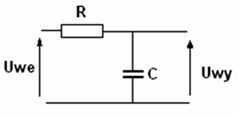
\includegraphics[width=0.4\linewidth]{RCdiagram4_12_1}
\caption{Filtr dolnoprzepustowy}
\label{fig:RCdiagram4}
\end{figure}
Dla układu jak na rysunku (\ref{fig:RCdiagram4}) wyznaczam transmitancję:

\begin{equation}
\left\lbrace \begin{array}{rcl}
u_{we} - u_R - u_{wy} &=& 0 \\
u_{R} &=& i  R \\
i &=& C  \frac{d u_{wy}}{dt} \\
\end{array}\right.
\end{equation}
 




\begin{align} 
u_{we} - RC \frac{d u_{wy}}{dt} - u_{wy} &= 0 \\
 \frac{d u_{wy}}{dt} + \frac{1}{RC}  u_{wy} &= \frac{1}{RC} u_{we}    \quad /\ \mathcal{L} \\
 s U_{wy} + \frac{1}{RC}  U_{wy} &= \frac{1}{RC} U_{we} \\
 U_{wy}  \left(  s+ \frac{1}{RC}\right) &=  \frac{1}{RC} U_{we} \\
\end{align}
w takim razie:
\begin{align} 
G(s)  = \frac{U_{wy}}{U_{we}} &= \frac{\frac{1}{RC}}{s+ \frac{1}{RC} }\\
 G(s) &= \frac{1}{1 + sRC} \\
\end{align}
Wzmocnienie to:




\begin{equation}
\frac{u_{wy}(t)}{u_{we}(t)} = |G(j\omega)| = \left| \frac{1}{1 + sRC} \right|  = \frac{1}{\sqrt{1 + \omega^2 R^2 C^2}}
\end{equation}

Wzmocnienie w decybelach:
\begin{align}
k = 20\log\left( \frac{u_{wy}}{u_{we}}\right)  &= 0 \; dB  \longleftarrow \text{ \it{jak inne wzmocnienie to tutaj wstawić}} \\
\log\left( \frac{u_{wy}}{u_{we}}\right)  &= 0  = \log(1)  \Longrightarrow \frac{u_{wy}}{u_{we}} = 1 \\
\end{align}
a zatem:
\begin{equation}
\frac{1}{\sqrt{1 + \omega^2 R^2 C^2}} = 1 \Longrightarrow \omega^2 R^2 C^2 = 0 \label{eq:wRC=0}
\end{equation}
Z założenia zadania:
\begin{align}
\omega &= 2\pi f \\
\omega &= 2 \pi \cdot 10^{-2} \left[ \frac{1}{s} \right] \longleftarrow \text{ \it{jak inna częstotliwość to tutaj wstawić}} \label{eq:w=2pi*f} \\
\end{align}

Z (\ref{eq:wRC=0}) i (\ref{eq:w=2pi*f}) wynika, że:
\begin{equation}
RC = 0 \quad \Longrightarrow \quad R=0 \vee C=0
\end{equation}
Wystarczy przyjąć, że $R = 0$ i $C$ jest dowolne

%###################                 4.13.1              #################################%

\subsection*{Zadanie 4.13.1}
Obliczyć przesunięcie fazowe przy pulsacji $0.5 \frac{rad}{s}$dla członu całkującego przy wzmocnieniu $-0.5 e$

\vspace{1em}

Człon całkujący daje na wyjściu sygnał $x(t)$ proporcjonalny do całki sygnału wejściowego $u(t)$.
\begin{align}
x(t) &= k \int_{0}^{t} u(\tau) \; d\tau \Longleftrightarrow X(s) = k \frac{1}{s} U(s) \\
G(s) &= \frac{k}{s} \\
k &= -\frac{e}{2} \Leftarrow \text{wynika z treści zadania} \\
 \label{eq:G(s)}G(s) &=  - \frac{e}{2s}
\end{align} 

Wiadomo, że układ  transmitancji $G(s)$ wprowadza przesunięcie fazowe:
\begin{equation}
\label{eq:phi}
\phi = \arg G(j\omega)
\end{equation}

Pulsacja układu na podstawie treści zadania wynosi:
\begin{equation}
\label{eq:omega}
 \omega = 0.5 \frac{rad}{s}
\end{equation}
Na podstawie (\ref{eq:G(s)}) ,  (\ref{eq:phi}) i  (\ref{eq:omega}):
\begin{equation}
\begin{split}
\phi = \arg G\left( \frac{1}{2} j\right)  = \arg \left( - \frac{e}{ 2 \cdot \frac{1}{2} j}  \right)   = \arg \left( - \frac{e}{j} \right) =  \\ \arg \left( - \frac{e}{j}\cdot \frac{j}{j} \right)  = \arg \left( - \frac{e j}{-1} \right) = \arg \left( e j \right) 
\end{split}
\end{equation}
Dla przypomnienia funkcja $\arg()$ to argument liczby zespolonej, czyli $ \arctan\left( \frac{b}{a}\right) $, gdzie $a$ to część rzeczywista, a $b$ to część zespolona.

W naszym przypadku mamy tylko cześć urojoną, a więc stosunek $ \frac{b}{a}$ jest równy $\infty$ 
\begin{equation}
\phi = \arg(ej) = \arctan(\infty) = \frac{\pi}{2}
\end{equation}


%`x(t) = k * całka (od 0 do t) u(tau) d(tau) <=> X(s) = k/s*U(s)
%G(s) = k/s
%W zadaniu k = -0.5 e = -e/2
%Wiadomo, że układ  transmitancji G(s) wprowadza przesunięcie fazowe fi = arg G(jw)
%Pulsacja układu to omega = 0.5 rad / s
%czyli fi = arg G(j * ½) = arg [ (-e/2)  / (j*1/2) ]  = arg (j*e/1) = arg (j*e) = pi/2
%Przesunięcie fazowe wprowadzane przez człon całkujący wynosi zatem pi/2


%###################                 4.10.2              #################################%
%\pagebreak
%\subsection*{Zadanie 4.10.2} {\color{darkgray}
%	Korzystając z kryterium Michajłowa zbadać stabilność asymptotyczną układu opisanego transmitancją $G(s)$:\\
%	$G(s)=\frac{s^2+s+1}{s^3-s^2+2s-2}$\\
%}\lineh
%\\\\

%  \left[\begin{array}{cc}\end{array}\right]
\pagebreak
\section*{Tydzień 5}
Wprowadzenie do układów nieliniowych - Linearyzacja\\
\\
\fbox{\parbox{.5\linewidth}{
\textbf{I metoda Lapunowa} \\
Punkt równowagi, dla którego system zlinearyzowany jest asymptotycznie stabilny jest lokalnie asymptotycznie stabilny. Jeżeli zaś chociaż jedna z wartości własnych macierzy systemu zlinearyzowanego ma dodatnią część rzeczywistą to punkt równowagi jest niestabilny.
}}\\
\\
\fbox{\parbox{.5\linewidth}{
\textbf{Macierz Hurwitz'a} \\
Wielomian charakterystyczny: $a_0\lambda^n+a_1\lambda^{n-1}+a_{n-1}\lambda+a_n$\\
$\left[ \begin{array}{cccccc}  
 a_1&a_3&a_5&a_7&\cdots&0\\
 a_0&a_2&a_4&a_6&\cdots&0\\
     0&a_1&a_3&a_5&\cdots&0\\
     0&a_0&a_2&a_4&\cdots&0\\
     0&    0&a_1&a_3&\cdots&0\\
\vdots&\vdots&\vdots&\vdots&\ddots&\vdots\\
0&0&0&0&\cdots&a_n
 \end{array}\right]$\\\\
\textbf{Kryterium Hurwitz'a} \\
Jeśli wszystkie minory wiodące są większe od zera, to jest asymptotycznie stabilny.
}}\\\\
\fbox{\parbox{.5\linewidth}{
\textbf{tw. Grobmana-Hartmana:}\\
Jeżeli $\det(j\omega I-J(x_r)) \neq 0, \ \ \ \omega \in \mathbb{R}, \ \ \ j^2=-1$\\
to trajektorie fazowe systemu nieliniowego w pewnym otoczeniu równowagi zachowują się podobnie jak trajektorie układu zlinearyzowanego w tym punktcie w otoczeniu zera. Warunek jest równoważny temu, że macierz $J(x_r)$ nie może posiadać wartości własnych na osi urojonej.
}}\\\\
\\
\textbf{Lapunowem zbadać stabilność punktów równowagi} \\
1. wyznaczamy punkt równowagi. Przyrównujemy równanie układu do zera.\\
2. Podstawiamy do macierzy Jacobiego punkt\\
$\left[ \begin{array}{cc}    \frac{\partial f_1}{\partial x_1} &\frac{\partial f_1}{\partial x_2} \\ \frac{\partial f_2}{\partial x_1} & \frac{\partial f_2}{\partial x_2}   \end{array}\right]$\\
3. Wyliczamy wartości własne macierzy Jacobiego i sprawdzamy czy ich część rzeczywista jest mniejsza od 0. Jeśli tak to punkt jest lokalnie asymptotycznie stabilny. Jeśli nie to punkt równowagi jest niestabilny.\\
Jeśli wyjdzie 0 to "Twierdzenie to nie rozstrzyga o stabilności punktu równowagi, jeżeli system zlinearyzowany jest jedynie stabilny"

\pagebreak
%###################                 5.1.1              #################################%
\subsection*{Zadanie 5.1.1} {\color{darkgray}
	Dany jest system dynamiczny\\
	$\dot{x}(t)= \cos(x(t))e^{-x(t)^2}$\\
	Wyznaczyć jego punkty równowagi i za pomocą I metody Lapunowa zbadać ich stabilność.\\
}\lineh
\\\\
$\dot{x}(t)=\cos(x(t))e^{-x(t)^2}$\\
$\dot{x}(t)=f(x(t))$\\
$x_r$ jest punktem równowagi $ \Leftrightarrow f(x_r)=0$\\
$f(x_r)=\cos(x_r)\cdot \underbrace{e^-x_r^2}_{<0}=0 \Rightarrow cos(x_r)=0 \Rightarrow x_r=\frac{\pi}{2}+k\pi, k \in \mathbb{Z}$\\
$\boxed{\begin{aligned}
\text{System zlinearyzowany: } \dot{x}(t)=J(x_r)x(t)\\
J(x)=\left[ \begin{array}{ccc} 
 \frac{\partial f_1}{\partial x_1}(x) & \cdots &  \frac{\partial f_1}{\partial x_n}(x)\\
\vdots & \ddots & \vdots\\
\frac{\partial f_n}{\partial x_1}(x) &\cdots & \frac{\partial f_n}{\partial x_n}(x) 
  \end{array}\right] f(x)= \left[ \begin{array}{c}  f_1(x)   \\ \vdots \\ f_n(x)    \end{array}\right]
\end{aligned}}$\\
$J(x)=\frac{\partial f}{\partial x} = - \sin(x) \cdot e^{-x^2}+\cos(x) \cdot (-2xe^{-x^2})=-e^{-x^2}(\sin(x)+2x\cos(x))$\\
$J(x_r)=\underbrace{-e^{-(\frac{\pi}{2}+k\pi)^2}}_{<0}(\underbrace{\sin(\frac{\pi}{2}+k\pi)}_{=1 \vee =-1})+\underbrace{2(\frac{\pi}{2}+k\pi)\cos(\frac{\pi}{2}+k\pi)}_{=0}=-e^{-(\frac{\pi}{2}+k\pi)^2} (\sin(\frac{\pi}{2}+k\pi))$\\
\\
\fbox{\parbox{.5\linewidth}{
\textbf{I metoda Lapunowa} \\
Punkt równowagi, dla którego system zlinearyzowany jest asymptotycznie stabilny jest lokalnie asymptotycznie stabilny. Jeżeli zaś chociaż jedna z wartości własnych macierzy systemu zlinearyzowanego ma dodatnią część rzeczywistą to punkt równowagi jest niestabilny.
}}\\
$\lambda = -e^{-(\frac{\pi}{2}+k\pi)^2}\cdot \sin(\frac{\pi}{2}+k\pi)$\\
\textbf{niestabilny :}\\
$ -e^{-(\frac{\pi}{2}+k\pi)^2}\cdot \sin(\frac{\pi}{2}+k\pi)>0 \Rightarrow \sin(\frac{\pi}{2}+k\pi)=-1 \Rightarrow x_r=\frac{\pi}{2}+(2k\pi+1)\pi,\ \  k \in \mathbb{Z}$\\
(z Hurwitza)\\
$-e^{-(\frac{\pi}{2}+k\pi)^2}\cdot \sin(\frac{\pi}{2}+k\pi)>0 \Rightarrow \sin(\frac{\pi}{2}+k\pi)= 1 \Rightarrow x_r=\frac{\pi}{2}+2k\pi,\ \  k \in \mathbb{Z}$\\
$ \left[ \begin{array}{cc}    1&0 \\0&   e^{-(\frac{\pi}{2}+k\pi)^2}\cdot \sin(\frac{\pi}{2}+k\pi) \end{array}\right]$

\pagebreak
%###################                 5.1.2              #################################%
\subsection*{Zadanie 5.1.2} {\color{darkgray}
	Dany jest system dynamiczny\\
	$\dot{x}_1(t)=x_2(t)$\\
	$\dot{x}_2(t)=-2x_1(t)-3x_1(t)^2-x_2(t)$\\
	Wyznaczyć jego punkty równowagi i za pomocą I metody Lapunowa zbadać ich stabilność.\\
}\lineh
\\\\
$J(x)=\left[ \begin{array}{cc}  0&1\\-2-6x_1 & -1   \end{array}\right]$\\
$\begin{cases}x_2=0\\-2x_1-3x_1^2-x_2=0\end{cases}$\\
$-2x_1-3x_1^2=0$\\
$x_1(2+3x_1)=0$\\
$x_1=0\ \  \vee \ \ x_1=-\frac23$\\
$\begin{array}{lll}
x_r= \left[ \begin{array}{c}   0\\0    \end{array}\right] &\ \ \ \vee \ \ \ & x_r= \left[ \begin{array}{c}   -\frac 23\\0    \end{array}\right] \\
J(x_r)=\left[ \begin{array}{cc}  0&1\\-2&-1    \end{array}\right] && J(x_r)=\left[ \begin{array}{cc}   0&1\\2&-1    \end{array}\right]\\
\left| \begin{array}{cc}  -\lambda & 1 \\-2&-1-\lambda    \end{array}\right|&&\left| \begin{array}{cc}  -\lambda & 1 \\2&-1-\lambda    \end{array}\right|\\
=(-\lambda)(-1-\lambda)+2=\lambda^2+\lambda+2&&=(-\lambda)(-1-\lambda)-2=\lambda^2+\lambda-2\\
\Delta=-7&&\Delta=9\\
\lambda=-\frac 12 \pm \frac{\sqrt 7}{2}i&&\lambda=\frac{-1 \pm 3}{2}\\
\lambda = -\frac 12 <0 \Rightarrow \text{Stabilny} && \lambda = 1 \ \ \vee \ \ \lambda=-2\\
 && \lambda = 1 >0 \Rightarrow \text{Niestabilny}
\end{array}$\\

%\begin{array}{c}\text{\circled{2}}\\x_r\end{array}

\pagebreak
%###################                 5.2.1              #################################%
\subsection*{Zadanie 5.2.1} {\color{darkgray}
	Wyznaczyć punkty równowagi układu generatora synchronicznego, który jest systemem dynamicznym opisanym następującymi równaniami\\
	$\dot{x}_1=x_2$\\
	$\dot{x}_2=-Dx_2-\sin x_1 + \sin \delta_0$\\
}\lineh
\\\\
$\begin{cases}\dot{x}_1=x_2 \\ \dot{x}_2=-Dx_2-\sin x_1 + \sin \delta_0 \end{cases}$\\
$f(x)= \left[ \begin{array}{c}   x_2  \\  -Dx_2-\sin x_1 + \sin \delta_0  \end{array}\right]$\\
$\left[ \begin{array}{c}   x_2  \\  -Dx_2-\sin x_1 + \sin \delta_0  \end{array}\right] = \left[ \begin{array}{c}  0\\0  \end{array}\right]$\\
$x_2=0$\\
$-\sin x_1 + \sin \delta_0 = 0 \Rightarrow \sin\delta_0=\sin x_1 \Rightarrow$\\
$\Rightarrow x_1=\delta_0+2k\pi \ \ \vee\ \  x_1=-\delta_0+(2k+1)\pi, \ \ \ k \in \mathbb{Z}$\\




\pagebreak
%###################                 5.2.2              #################################%
\subsection*{Zadanie 5.2.2} {\color{darkgray}
	Wyznaczyć punkty równowagi dla obwodu Chuy, który jest systemem dynamicznym opisanym następującymi równaniami:\\
	$C_1\dot{x}_1(t)=-\frac 1R x_1(t)+\frac 1R x_2(t)-g(x_1(t))$\\
	$C_2\dot{x}_2(t)= \frac 1R x_1(t) -\frac 1R x_2(t)+x_3(t)$\\
	$L\dot{x}_3(t)=-x_2(t)-R_0x_3(t)$\\
	przy czym $g(v)=g_1v+g_2v^3$\\
}\lineh
\\\\
$\begin{cases} 
-\frac{1}{RC_1}x_1+\frac{1}{RC_1}x_2-\frac{g_1}{C_1}x_1-\frac{g_2}{C_1}x_1^3=0\\
\frac{1}{RC_2}x_1 -\frac{1}{RC_2}x_2+\frac{x_3}{C_2}=0\\
-\frac 1Lx_2 -\frac{R_0}{L}x_3=0 \ \ \ \ \ \ \ \ \ \ \ \Rightarrow x_2=-R_0x_3
\end{cases}$\\
$\begin{cases} 
g_1Rx_1+g_2Rx_1^3+x_1=x_2\\
x_1+Rx_3=x_2\\
x_2=-R_0x_3
\end{cases}$\\
z drugiego i trzeciego:\\
$x_3=\frac{-x_1}{R+R_0}$\\
z pierwszego i drugiego:\\
$g_1Rx_1+g_2Rx_1^3=Rx_3$\\
$g_1x_1+g_2x_1^3=x_3$\\
podstawiam $x_3$ z trzeciego:\\
$g_1x_1+g_2x_1^3=\frac{-x_1}{R+R_0}$\\
$g_1x_1+x_1^3g_2+\frac{x_1}{R+R_0}=0$\\
$x_1^3g_2+x_1(g_1+\frac{1}{R+R_0})=0$\\
podstawiam pomocnicze zmienne:\\
$a = g_2, \ \ \ b=g_1+\frac{1}{R+R_0}$\\
$ax_1^3+bx_1=0$\\
$x_1(ax_1^2+b)=0$\\
$\begin{array}{lll}   
\circled{1} \ x_1=0 & \ \ \vee \ \ & ax_1^2+b=0\\
&&\circled{2} \ x_1=\sqrt{\frac{-b}{a}} \ \ \vee \ \  \circled{3} \ x_1=-\sqrt{\frac{-b}{a}}
 \end{array}$\\
podstawiam $x_1=0$:\\
$x_r=\left[ \begin{array}{c}   x_{1r}\\ x_{2r}\\x_{3r}   \end{array}\right]
=\left[ \begin{array}{c}   x_{1}\\ x_{2}\\x_{3}   \end{array}\right]$\\\\
$\circled{1} \ x_r=\left[ \begin{array}{c}   0\\0\\0   \end{array}\right]$\\\\\\
$\circled{2} \ x_r=\left[ \begin{array}{c}   
	\sqrt{\frac{-g_1-\frac{1}{R+R_0}}{g_2}}\\
\\
	-R_0\frac{-\sqrt{\frac{-g_1-\frac{1}{R+R_0}}{g_2}}}{R+R_0}   \\
\\
	\frac{-\sqrt{\frac{-g_1-\frac{1}{R+R_0}}{g_2}}}{R+R_0}
\end{array}\right]$\\\\\\
$\circled{3} \ x_r=\left[ \begin{array}{c}   
	-\sqrt{\frac{-g_1-\frac{1}{R+R_0}}{g_2}}\\
\\
	-R_0\frac{\sqrt{\frac{-g_1-\frac{1}{R+R_0}}{g_2}}}{R+R_0}   \\
\\
	\frac{\sqrt{\frac{-g_1-\frac{1}{R+R_0}}{g_2}}}{R+R_0}
\end{array}\right]$



\pagebreak
%###################                 5.3.1              #################################%
\subsection*{Zadanie 5.3.1} {\color{darkgray}
	Dla jakich wartości parametru $\epsilon$ zerowy punkt równowagi układu zwanego oscylatorem Van der Pola będzie niestabilny\\
	$\ddot{x}(t)-\epsilon(1-x(t)^2)\dot{x}(t)+x(t)=0$\\\\
}\lineh
\\\\
$\begin{cases} x_1=x \\ x_2 =\dot{x} \end{cases} \begin{cases} \dot{x}_1=\dot{x}=x_2 \\ \dot{x}_2=\ddot{x}= \epsilon(1-x(t)^2) \cdot \dot{x}(t)-x(t)=\epsilon(1-x_1^2) \cdot x_2 - x_1 \end{cases}$\\
$f(x)=\left[ \begin{array}{c}   x_2  \\  \epsilon(1-x_1^2) \cdot x_2 - x_1  \end{array}\right] = \left[ \begin{array}{c}  f_1(x)   \\ f_2(x)   \end{array}\right]$\\
$\begin{cases} x_2=0 \\ \epsilon(1-x_1^2) \cdot x_2 - x_1 = 0\end {cases} \Rightarrow \begin{cases}x_2=0 \\ x_1 = 0 \end {cases} \ \ \ x_r = \left[ \begin{array}{c}     0\\0   \end{array}\right]$\\
$J(x)=\left[ \begin{array}{cc}   0 &1  \\ -2\epsilon x_1 x_2 -1 & \epsilon(1-x_1^2)   \end{array}\right] \ \ \ \ \ \ \ 
{\color{lightgray}\boxed{\left[ \begin{array}{cc}    \frac{\partial f_1}{\partial x_1} &\frac{\partial f_1}{\partial x_2} \\ \frac{\partial f_2}{\partial x_1} & \frac{\partial f_2}{\partial x_2}   \end{array}\right]}}$\\
$J(x_r)= \left[ \begin{array}{cc}    0&1 \\-1 & \epsilon    \end{array}\right]$\\
Z Lapunowa:\\
$(- \lambda)(\epsilon - \lambda)+1 = \lambda^2 - \lambda \epsilon +1 = 0$\\
$\Delta = \epsilon^2-4 \Rightarrow \lambda =\frac{\epsilon \pm \sqrt{\epsilon^2-4}}{2}$\\
niestabilny: Jeżeli część rzeczywista $>0 \Rightarrow \frac{\epsilon}{2}>0 \Rightarrow \boxed{\epsilon >0}$\\
asymptotycznie stabilny : $\left[ \begin{array}{cc}    -\epsilon & 0 \\ 1 & 1   \end{array}\right]$ Hurwitz $-\epsilon>0 \Rightarrow \boxed{\epsilon<0}$\\



\pagebreak
%###################                 5.4.1              #################################%
\subsection*{Zadanie 5.4.1} {\color{darkgray}
	Dla jakich wartości parametru $a$ linearyzacja przestaje spełniać warunki twierdzenia Grobmana-Hartmana dla układu opisanego równaniami:\\
	$\dot{x_1}(t)=-x_2(t)+(a-x_1(t)^2-x_2(t)^2)x_1(t)$\\
	$\dot{x_2}(t)=x_1(t)+(a-x_1(t)^2-x_2(t)^2)x_2(t)$\\\\
}\lineh
\\\\
$\dot{x_1}(t)=-x_2(t)+(a-x_1(t)^2-x_2(t)^2)x_1(t)=f_1(x(t))$\\
$\dot{x_2}(t)=x_1(t)+(a-x_1(t)^2-x_2(t)^2)x_2(t)=f_2(x(t))$\\
$f(x)=\left[ \begin{array}{c}     f_1(x) \\ f_2(x)   \end{array}\right]$\\
$\begin{cases} -x_2+(a-x_1^2-x_2^2)x_1=0 \\ x_1+(a-x_1^2-x_2^2)x_2=0\end{cases}  $\\
Zauważamy, że albo $x_1=x_2=0$ albo dla $x_2 \neq 0 \wedge x_1 \neq 0$ :\\
$\begin{cases} -\frac{x_2}{x_1}+(a-x_1^2-x_2^2)=0 \\ \frac{x_1}{x_2}+(a-x_1^2-x_2^2)=0\end{cases}  \Rightarrow \frac{-x_2}{x_1} = \frac{x_1}{x_2} \Rightarrow -x_2^2=x_1^2 \Rightarrow x_1=x_2=0$ (sprzeczność)\\
więc $x_r=\left[ \begin{array}{c}     0\\0   \end{array}\right]$\\
$J(x)=\left[ \begin{array}{cc}   a-3x_1^2-x_2^2 & -1-2x_2x_1 \\ 1-2x_1x_2 & a-x_1^2-3x_2^2    \end{array}\right]$\\
$J(x_r)=\left[ \begin{array}{cc}    a & -1 \\ 1 & a    \end{array}\right]$\\
z tw. Grobmana-Hartmana:\\
$\begin{array}{ll}
\det(j\omega I-J(x_r)) \neq 0, \ \ \ \omega \in \mathbb{R} & J(x_r)\text{ nie ma wartości własnych na osi urojonej}\\
 \left| \begin{array}{cc}     j\omega-a& -1 \\ 1 & j\omega-a    \end{array}\right|=0 &  \left[ \begin{array}{cc}    a-\lambda & -1 \\ 1 & a- \lambda   \end{array}\right]\\
(j\omega-a)^2+1=0 & (a-\lambda)^2+1=0\\
j\omega-a= \pm j \Rightarrow \boxed{ a=0} & a^2-2a\lambda +\lambda^2+1 =0\\
&\lambda^2-2a\lambda+a^2+1 = 0\\
&\Delta=4a^2-4a^2-4\\
&\sqrt{\Delta}=2i\\
&\lambda=\frac{2a \pm 2i}{2} = a \pm i\\
&\text{dla } a=0 \text{ wartości własne są na osi urojonej}
\end{array}$\\


\pagebreak
%###################                 5.5.1              #################################%
\subsection*{Zadanie 5.5.1} {\color{darkgray}
	Dla jakich wartości parametru $a$ zerowy punkt równowagi układu opisanego równaniami\\
	$\dot{x_1}(t)=x_2(t)+(a-x_1(t)^2-x_2(t)^2)x_1(t)$\\
	$\dot{x_2}(t)=x_1(t)+(a-x_1(t)^2-x_2(t)^2)x_2(t)$\\
	będzie niestabilny.\\
}\lineh
\\\\
$x_r=\left[ \begin{array}{c}     0\\0   \end{array}\right]$\\
$J(x)=\left[ \begin{array}{cc}    a-3x_1^2 -x_2^2&  1-2x_2x_1 \\ 1-2x_1x_2 & a-x_1^2-3x_2^2  \end{array}\right]$\\
$J(x_r)=\left[ \begin{array}{cc}    a&1\\1&a  \end{array}\right]$\\
$\left| \begin{array}{cc}    a-\lambda&1\\1&a-\lambda  \end{array}\right| =0$\\
$(a-\lambda)^2-1=0$\\
$(a-\lambda-1)(a-\lambda+1)=0$\\
$\lambda=a-1 \ \ \ \vee \ \ \ \lambda=a+1$\\
niestabilny, gdy $Re(\lambda)>0$\\
$\begin{array}{lll}     a-1>0& \ \ \  &a+1>0  \\ a>1 && a>-1 \end{array}$\\
$(a>1 \ \ \vee \ \ a>-1 ) \Rightarrow \boxed{a>-1}$\\
\\
{\color{red} \textbf{ Alternatywnie: Bez podanego punktu równowagi}}\\
$\dot{x_1}(t)=x_2(t)+(a-x_1(t)^2-x_2(t)^2)x_1(t)=f_1(x(t))$\\
$\dot{x_2}(t)=x_1(t)+(a-x_1(t)^2-x_2(t)^2)x_2(t)=f_2(x(t))$\\
$f(x)= \left[ \begin{array}{cc}    f_1(x)\\f_2(x)    \end{array}\right]$\\
$\begin{cases}x_2+(a-x_1^2-x_2^2)x_1=0 \\ x_1+(a-x_1^2-x_2^2)x_2=0\end{cases}$\\
Zauważamy, że albo $x_1=x_2=0$ albo dla $x_1\neq 0 \wedge x_2 \neq 0 $ :\\
$\begin{cases} \frac{x_2}{x_1}+(a-x_1^2-x_2^2)=0 \\ \frac{x_1}{x_2}+(a-x_1^2-x_2^2)=0\end{cases} 
\Rightarrow \frac{x_2}{x_1}=\frac{x_1}{x_2} \Rightarrow 
\begin{array}{c}x_2^2 = x_1^2 \\x_1=x_2 \vee x_1=-x_2 \end{array}$\\
więc $\begin{array}{c}\text{\circled{1}}\\x_r\end{array}=\left[ \begin{array}{c} k\\k\end{array}\right] \vee
\begin{array}{c}\text{\circled{2}}\\x_r\end{array}=\left[ \begin{array}{c} k\\-k\end{array}\right],  \ \ \ k \in \mathbb{R}$\\
$J(x)=\left[ \begin{array}{cc}    a-3x_1^2 -x_2^2&  1-2x_2x_1 \\ 1-2x_1x_2 & a-x_1^2-3x_2^2  \end{array}\right]$\\
$\begin{array}{lll}
J( \begin{array}{c}\text{\circled{1}}\\x_r\end{array})= \left[ \begin{array}{cc}  a-4k^2 & 1-2k^2 \\1-2k^2 & a-4k^2 \end{array}\right] &\vee&
J( \begin{array}{c}\text{\circled{2}}\\x_r\end{array})= \left[ \begin{array}{cc}  a-4k^2 & 1+2k^2 \\1+2k^2 & a-4k^2 \end{array}\right]\\
(a-4k^2-\lambda)^2-(1-2k^2)^2=0         &\vee&       (a-4k^2-\lambda)^2-(1+2k^2)^2=0 \\
(a-4k^2-\lambda-1+2k^2)(a-4k^2-\lambda+1-2k^2)=0 &\vee& (a-4k^2-\lambda-1-2k^2)(a-4k^2-\lambda+1+2k^2)=0 \\
\lambda = a-1-2k^2 \vee \lambda=a+1-6k^2 &\vee& \lambda = a-1-6k^2 \vee \lambda=a+1-2k^2 \\
niestebilny:&&\\
Re \lambda >0 &&\\
a-1-2k^2>0 \vee a+1-6k^2>0 &&a-1-6k^2>0 \vee a+1-2k^2>0\\
\begin{array}{c}\text{\circled{1}}\\a>1+2k^2\end{array}
\begin{array}{c}\text{\circled{2}}\\a>6k^2-1\end{array} && 
\begin{array}{c}\text{\circled{3}}\\a>1+6k^2\end{array}
\begin{array}{c}\text{\circled{4}}\\a>2k^2-1\end{array}
\end{array}$\\
odp. niestabilny dla $a>\circled{1} \vee a>\circled{2} \vee a>\circled{3} \vee a>\circled{4} $\\



\pagebreak
%###################                 5.5.2              #################################%
\subsection*{Zadanie 5.5.2} {\color{darkgray}
	Dla jakich wartości parametru $a$ zerowy punkt równowagi układu opisanego równaniami\\
	$\dot{x_1}(t)=-x_2(t)+(a-x_1(t)^2-x_2(t)^2)x_1(t)$\\
	$\dot{x_2}(t)=x_1(t)+(a-x_1(t)^2-x_2(t)^2)x_2(t)$\\
	będzie niestabilny.\\
}\lineh
\\\\
$x_r=\left[ \begin{array}{c}     0\\0   \end{array}\right]$\\
$J(x)=\left[ \begin{array}{cc}   a-3x_1^2-x_2^2 & -1-2x_2x_1 \\ 1-2x_1x_2 & a-x_1^2-3x_2^2    \end{array}\right]$\\
$J(x_r)=\left[ \begin{array}{cc}    a & -1 \\ 1 & a    \end{array}\right]$\\
$\left| \begin{array}{cc}     a-\lambda & -1 \\ 1 & a-\lambda   \end{array}\right|=0$\\
$\lambda^2-2a\lambda+a^2+1=0$\\
$\Delta=-4$\\
$\lambda = \frac{2a \pm 2i}{2}=a \pm i$\\
niestabilny, gdy $Re(\lambda)>0$\\
$\boxed{a>0}$\\



\pagebreak
%###################                 5.6.1              #################################%
\subsection*{Zadanie 5.6.1} {\color{darkgray}
	Dla jakich wartości parametru $a$ zerowy punkt równowagi układu opisanego równaniami\\
	$\dot{x_1}(t)=-x_2(t)+(a-x_1(t)^2-x_2(t)^2)x_1(t)$\\
	$\dot{x_2}(t)=x_1(t)+(a-x_1(t)^2-x_2(t)^2)x_2(t)$\\
	będzie asymptotycznie stabilny.\\
}\lineh
\\\\
$x_r=\left[ \begin{array}{c}     0\\0   \end{array}\right]$\\
$J(x)=\left[ \begin{array}{cc}   a-3x_1^2-x_2^2 & -1-2x_2x_1 \\ 1-2x_1x_2 & a-x_1^2-3x_2^2    \end{array}\right]$\\
$J(x_r)=\left[ \begin{array}{cc}    a & -1 \\ 1 & a    \end{array}\right]$\\
$\left| \begin{array}{cc}     a-\lambda & -1 \\ 1 & a-\lambda   \end{array}\right|=0$\\
$\lambda^2-2a\lambda+a^2+1=0$\\
\fbox{\parbox{.5\linewidth}{
\textbf{Macierz Hurwitz'a} \\
Wielomian charakterystyczny: $a_0\lambda^n+a_1\lambda^{n-1}+a_{n-1}\lambda+a_n$\\
$\left[ \begin{array}{cccccc}  
 a_1&a_3&a_5&a_7&\cdots&0\\
 a_0&a_2&a_4&a_6&\cdots&0\\
     0&a_1&a_3&a_5&\cdots&0\\
     0&a_0&a_2&a_4&\cdots&0\\
     0&    0&a_1&a_3&\cdots&0\\
\vdots&\vdots&\vdots&\vdots&\ddots&\vdots\\
0&0&0&0&\cdots&a_n
 \end{array}\right]$\\
}}\\\\\\
$\left[ \begin{array}{cc}   -2a & 0 \\ 1 & a^2+1    \end{array}\right]$\\\\\\
\fbox{\parbox{.5\linewidth}{
\textbf{Kryterium Hurwitz'a} \\
Jeśli wszystkie minory wiodące są większe od zera, to jest asymptotycznie stabilny.
}}\\\\
$-2a>0 \Rightarrow a<0$\\
$-2a(a^2+1)>0 \Rightarrow \boxed{a<0}$\\

%  \left[ \begin{array}{c}     \\    \end{array}\right] 

\pagebreak
\section*{Autorzy:}

\subsection*{Skład:} 
Jacek Pietras\\
Grzegorz Tokarz\\
Jakub Hyła

\subsection*{Rozwiązania:} 
Magdalena Warzesia\\
Ania Szarawara\\
irytek102\\
Gniewomir\\
Jacek Pietras\\
Grzegorz Tokarz\\
Magdalena Jaroszyńska

\subsection*{Komentarze:} 
\end{document}


%  \left[\begin{array}{cc}     &\\&    \end{array}\right]
%  \left[\begin{array}{c}     \\    \end{array}\right]



